% /* cspell:disable */
\documentclass[a4paper,12pt]{book}

% import package
\usepackage{graphics}   % include graphics
\usepackage{float}      % h!

% font
\usepackage{helvet}
\usepackage{color}
\renewcommand{\familydefault}{\sfdefault}


% caption
\usepackage[labelfont=bf,font=sf]{caption}
\DeclareCaptionFont{caption_size}{\fontsize{12}{13}\rmfamily}
\captionsetup{font=caption_size}

% figure
\usepackage{tikz}
\usepackage{pgfplots}
\usepackage{graphicx}
\usepackage{subcaption}

% page
\usepackage{fancyhdr}
\usepackage{setspace}
\usepackage{sectsty}

% reference
\usepackage[sort&compress]{natbib}

% math
\usepackage{amssymb}
\usepackage{amsmath}
\usepackage{breqn}          % dmath
\usepackage{siunitx}

%algorithm
% \usepackage{algorithm,algorithmicx,algpseudocode}
\usepackage[linesnumbered,ruled]{algorithm2e}
\SetKwRepeat{Do}{do}{while}
\SetKwInOut{Input}{Input}
\SetKwInOut{Output}{Output}

% fancyhdr setting
\pagestyle{fancy}
\fancyhead{}
\fancyhead[LO]{\bfseries\rightmark}
\fancyhead[RO]{}
\fancyhead[RE]{\bfseries\leftmark}
\fancyhead[LE]{}

%table
\usepackage{multirow}
\usepackage{booktabs}
\usepackage{tabularx}


% page setting
\doublespacing
\allsectionsfont{\singlespacing}
\raggedbottom
\setcounter{secnumdepth}{3}

% math symbols
\DeclareMathOperator*{\argmin}{arg\,min}
\DeclareMathOperator*{\argmax}{arg\,max}
\newcommand*\mean[1]{\overline{#1}}
\newcommand{\RN}[1]{
    \textup{\uppercase\expandafter{\romannumeral#1}}
}

%pdf plot
% \pgfplotsset{compat=1.15}
\begin{document}
% roman page numbering for first few parts
\pagenumbering{roman}
% !TeX root = ./thesis.tex
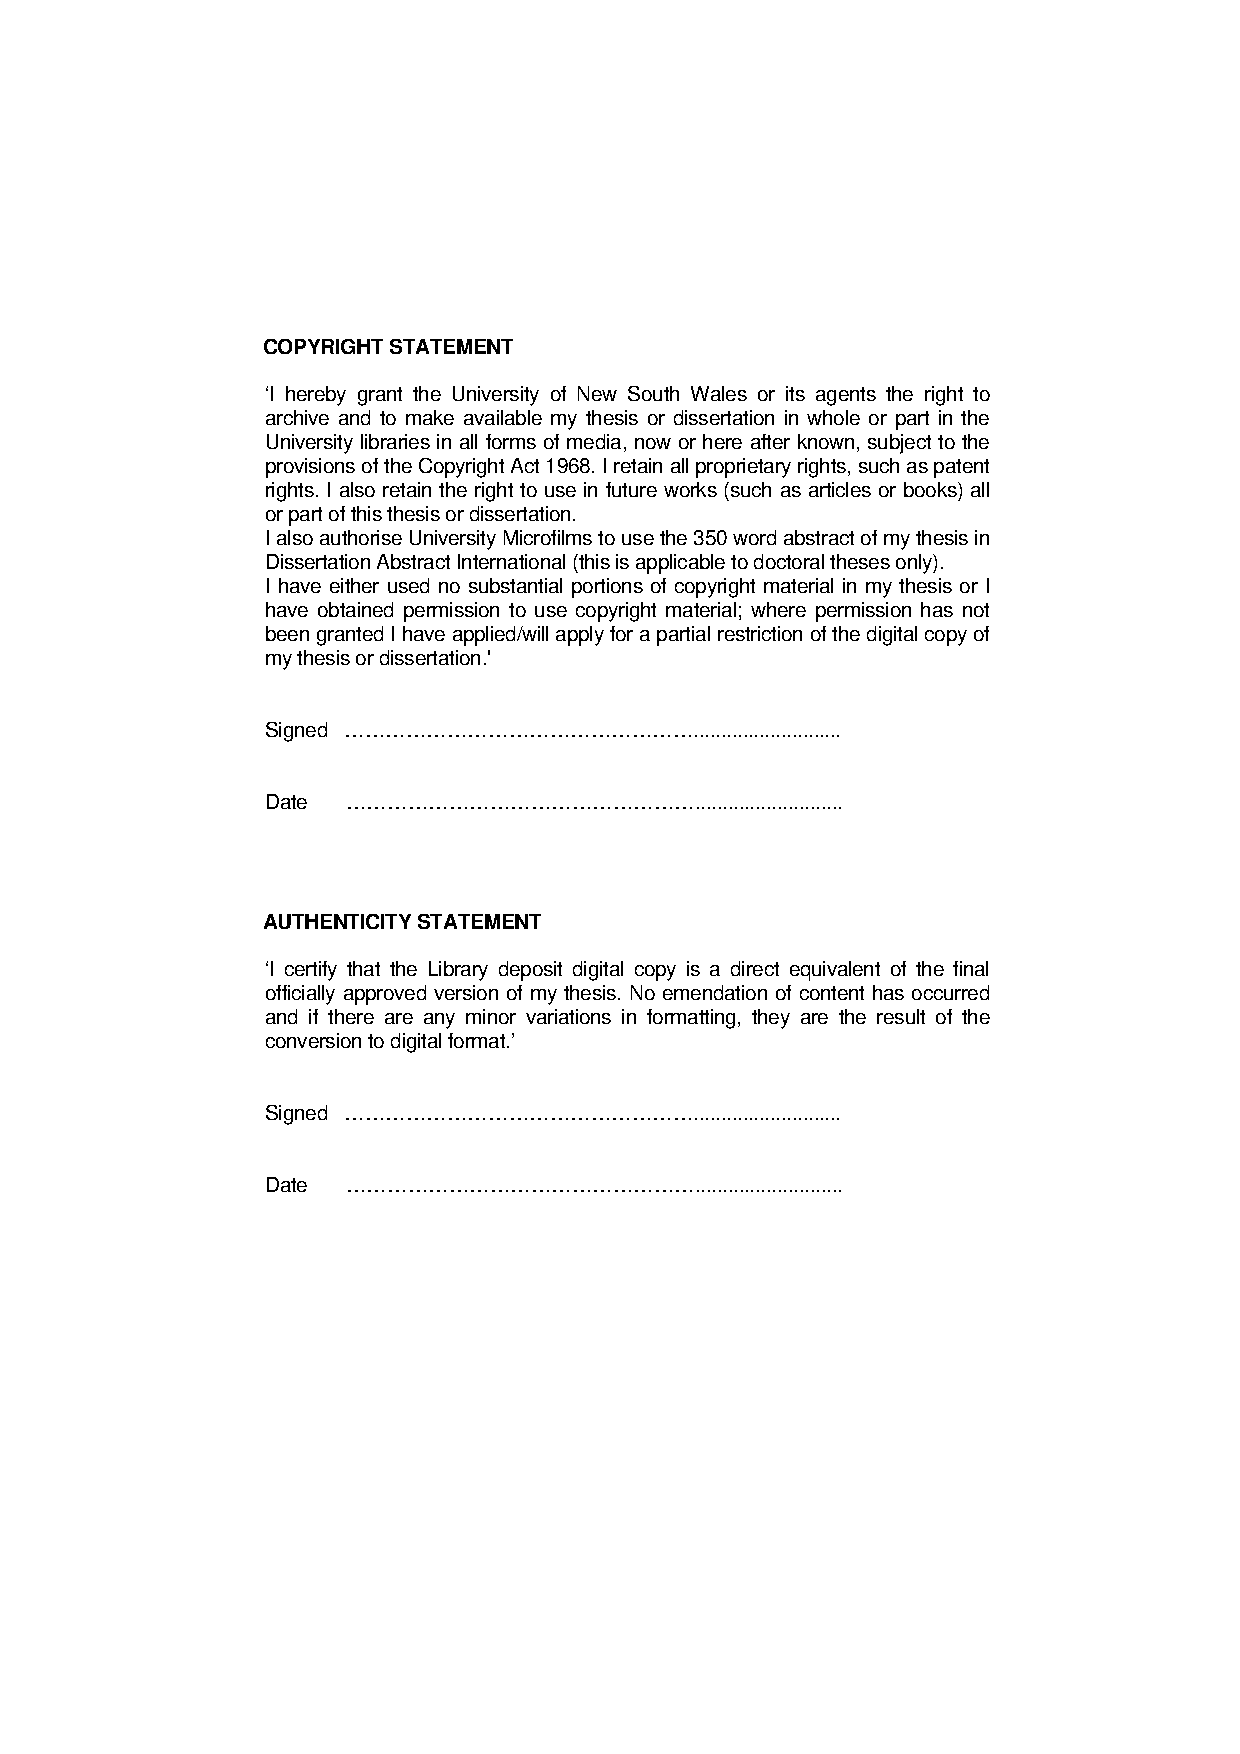
\includepdf[pages=-]{copyrightauthenticitystatements.pdf}
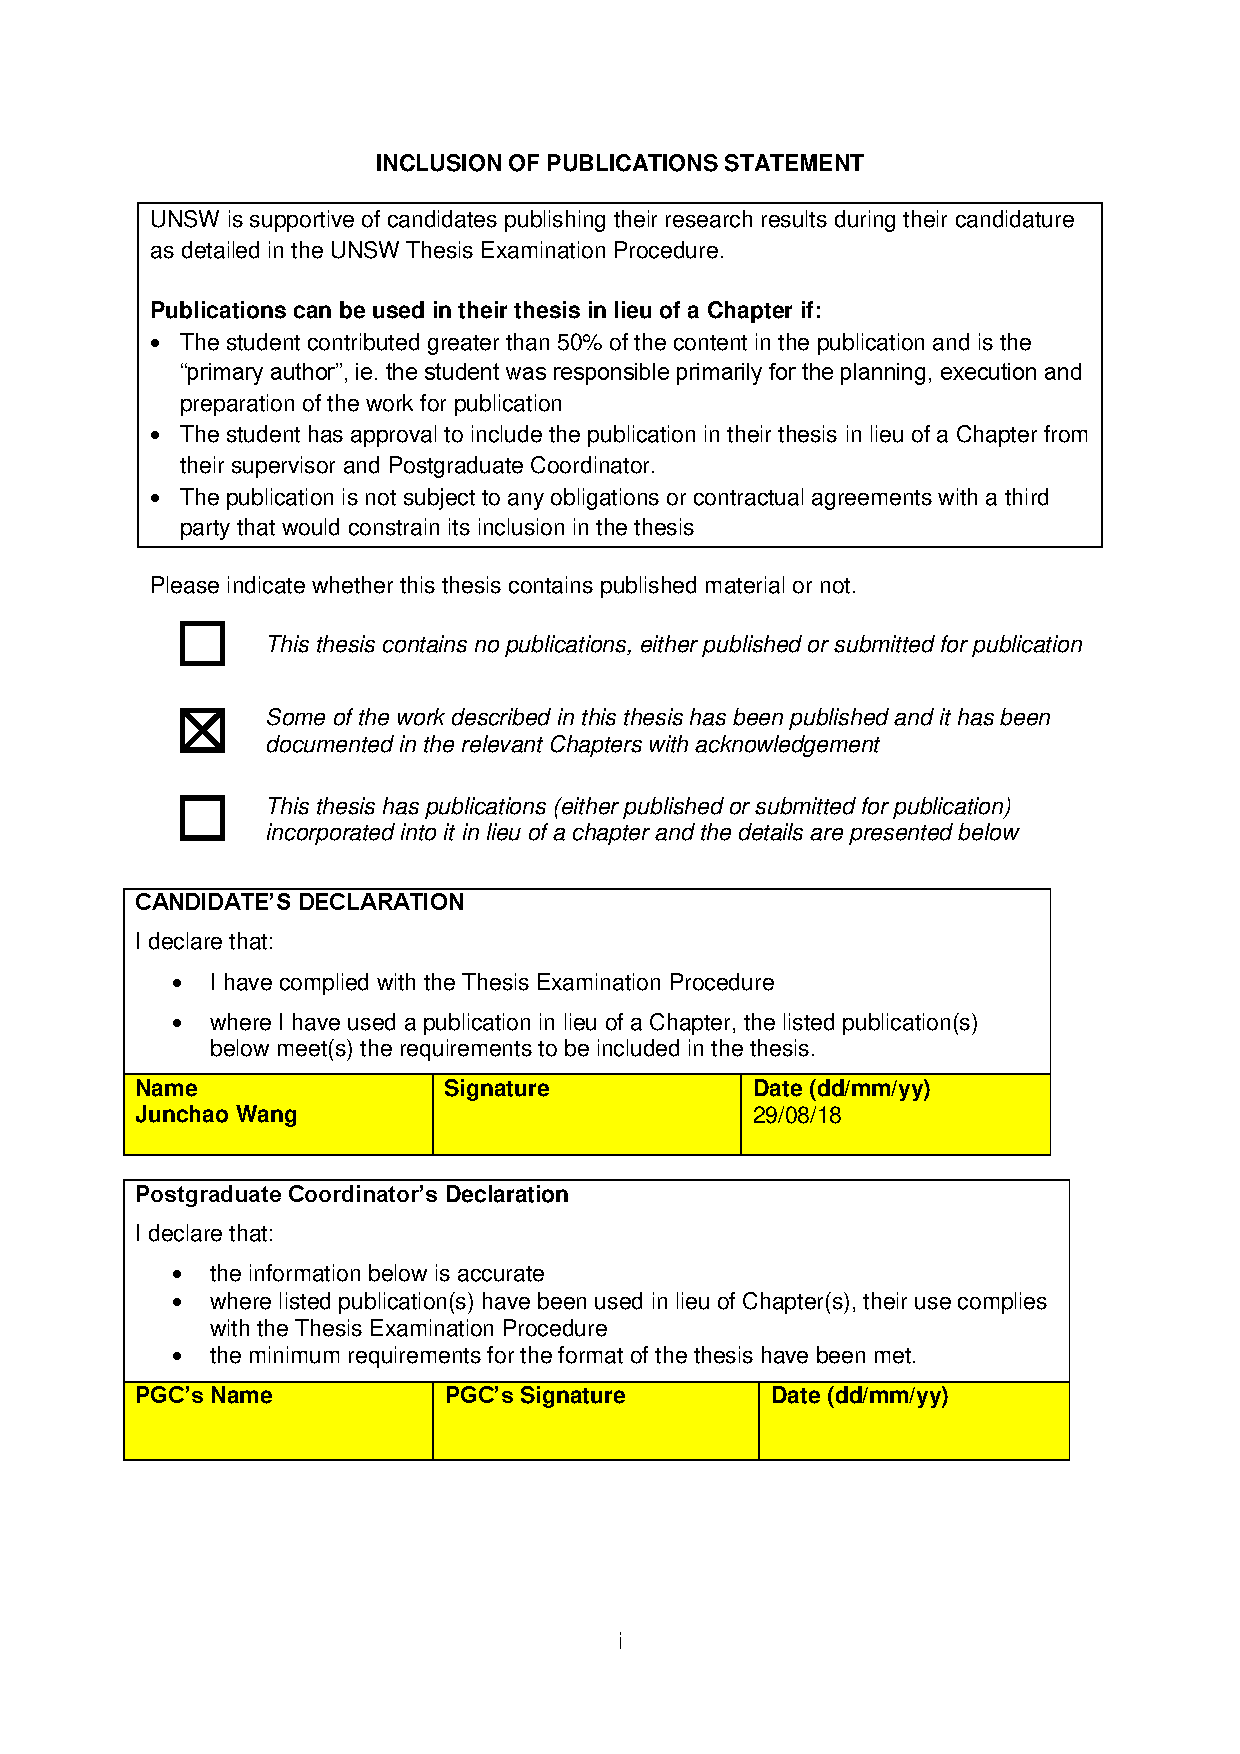
\includepdf[pages=-]{Inclusion_of_publications_statement.pdf}
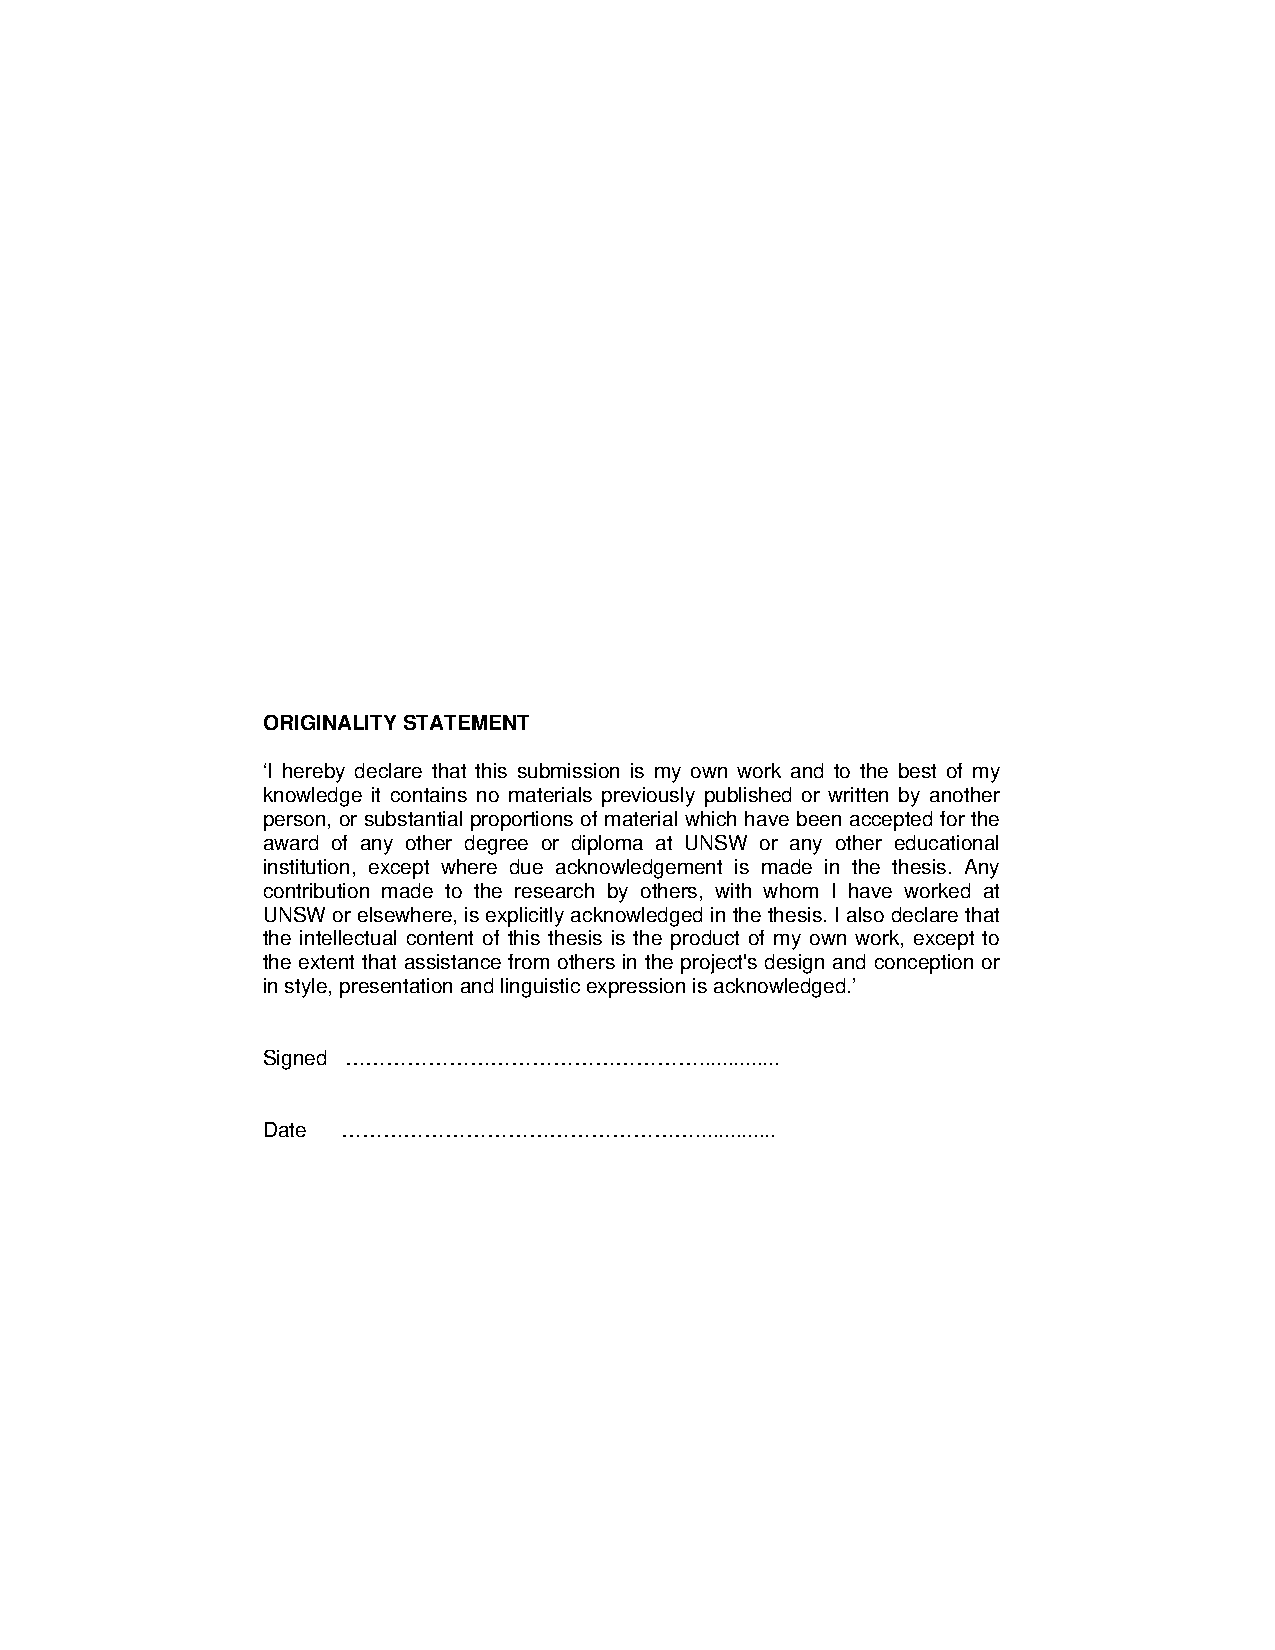
\includepdf[pages=-]{originalitystatement.pdf}

\chapter*{Acknowledgement}
\addcontentsline{toc}{chapter}{Acknowledgement}
\paragraph{}
Foremost, I would like to express my sincere gratitude to my supervisor Prof. Chongmin Song and Dr.Sundararajan Natarajan for the continuous support of my research, for their patience, motivation, enthusiasm, and immense knowledge.
their guidance helped me in all the time of research and writing of this thesis.
I could not have imagined having a better advisor and mentor for my Ph. D Thesis.

% ------------------------------------------------------------- %

\chapter*{Abstract}
\addcontentsline{toc}{chapter}{Abstract}
\paragraph{}
The Finite element method (FEM) constitutes a general tool for the numerical solution of partial differential equations in engineering and applied science.
Great amount of research has been conducted on FEM in terms of mathematics and applications, contributing to its dominance over numerical method in solid mechanics and structural analysis.
Although it is a principle method for solving complex problems in the engineering field, deficiency in geometric representation has been detected.
Besides, it could be expensive in terms of time and human resource to create the mesh required by the FEM.
The research towards integrating geometry and analysis has led to the ‘Isogeometric Analysis’ (IGA) (Hughes et al., 2005).
However, as the CAD model provides information only of the boundary, a 2D/3D stress analysis is still one major step away.

\paragraph{}
This thesis presents a simple and efficient technique based on the combination of the scales boundary finite element method (SBFEM), automatic mesh generation and adaptive refinement algorithms to reduce the human efforts in the structural analysis.
In the SBFEM, only the boundary information is required and hence a seamless integration can be provided with the CAD modelling.
The NURBS basis functions are adopted to discretize the unknown fields in the circumferential direction within the proposed framework, whilst analytical solution is sought in the radial direction.
This framework will also be further extended to problems with singularities and to dynamic analysis.

\paragraph{}
To mode problems with complex geometries, the problems domains are divided into a mesh of scaled boundary finite elements.
A quad-tree based mesh generation algorithm is developed. High quality mesh will be generated with the help of the algorithm and the computational cost will also be improved due to the utilization of the patterns in the quad-tree.
Furthermore, no human efforts are required for the pre-processing as the output of the CAD software (i.e. IGES file) will be used to determine the geometric information automatically.
Any mismatch between the geometric representation in design and in numerical analysis may be prevented as the design is used directly.

\paragraph{}
To ensure a controllable accuracy and minimal computational cost, an adaptive and robust mesh refinement algorithm is also developed to prevent unnecessary refinement in the region which contributes little to the improvement to the accuracy.
The expressions related to the eigenvalues of the SBFEM formulation representing the quantity of the error in the interpolation are adopted as one of the error indicators, together with the area and other geometric properties of the Scaled Boundary Finite Element.
A machine learning model using the Multilayer Perceptron (MLP) is trained to determine whether a Scaled Boundary Finite Element needs refinement or not based on all these information.

\paragraph{}
The proposed method is further extended to 3D with an initial mesh generated based on the STL file and octree algorithm.
The octree mesh provides a high quality mesh in 3D for SBFEM and the IGES file from the CAD software will be adopted in order to map intersection points back to NURBS surfaces to preserve an exact geometry.
The convex hull properties of the NURBS are utilized to accelerate the algorithm.

\paragraph{}
Numerical examples are presented to verify the proposed technique with the results from the literature and the numerical results obtained using the commercial software ANSYS.
The accuracy and the convergence properties of the proposed method are demonstrated with benchmark problems in the context of linear elasticity and linear elastic fracture mechanics.
The presented results show a higher accuracy and rate of convergence of the proposed method.

% ------------------------------------------------------------- %

\chapter*{Publications}
\section*{Journal papers}
\begin{enumerate}
    \item Sundararajan Natarajan, \textbf{JunChao Wang} , Chongmin Song , Carolin Birk (2015).
    Isogeometric analysis enhanced by the scaled boundary finite element method.
    \textit{Computer Methods in Applied Mechanics and Engineering}, 283:733-762
    \item Yan Liu , Albert A. Saputra, \textbf{Junchao Wang}, Francis Tin-Loi, Chongmin Song (2017).
    Automatic polyhedral mesh generation and scaled boundary finite element analysis of STL models.
    \textit{Computer Methods in Applied Mechanics and Engineering}, 313:106-132
\end{enumerate}

% ------------------------------------------------------------- %

\chapter*{Nomenclature}
\addcontentsline{toc}{chapter}{Nomenclature}
\renewcommand{\arraystretch}{2}
\begin{table}[h!]
\begin{tabular}{lr}
    {\it Greek Letters}     &   \\
    $\epsilon$              &   Threshold   \\
    $\{ \epsilon \}$        &   Strain tensor   \\
    $\zeta(x)$              &   Softplus function   \\
    $\kappa$                &   Kolosov constants   \\
    $\lambda$               &   Eigenvalue  \\
    $\nu$                   &   Poisson's ratio \\
    $( \xi, \eta, \zeta )$  &   Scaled boundary finite element coordinates  \\
    $\{ \Xi \}$             &   NURBS knot vector   \\
    $\rho$                  &   Density \\
    $\sigma$                &   Logistic sigmoid    \\
    $\{ \sigma \}$          &   Stress tensor   \\
    $\{ \Phi \}$            &   Surface tractions   \\
    $\{ \psi_\sigma \}$     &   Stress mode \\
\end{tabular}
\end{table}
\pagebreak
\renewcommand{\arraystretch}{1.4}

\begin{longtable}{lr}
    % \begin{tabular}{lr}
        {\it Latin Letters}                 &   \\
        $\{B\}$                             &   Minibatch   \\
        $\{c\}$                             &   Integrating constants   \\
        $\{C(u)\}$                          &   NURBS curve \\
        $E$                                 &   Young's modulus \\
        $E_{a \sim b}$                      &   Cross entropy between data set $a$ and $b$  \\
        $[E_0], [E_1], [E_2]$               &   Element coefficient matrices    \\
        $\{F\}$                             &   Nodal forces    \\
        $G$                                 &   Shear modulus   \\
        $J(\theta)$                         &   Cost function   \\
        $|J|$                               &   Determinant of Jacobian matrix  \\
        $[J(\xi, \eta, \zeta)]$             &   Jacobian matrix \\
        $K_{\mathrm{I}}, K_{\mathrm{II}}$   &   Stress intensity factors for mode $\mathrm{I}$ and $\mathrm{II}$    \\
        $[K]$                               &   Stiffness matrix    \\
        $L(x, y, \theta)$                   &   Pre-example Loss function   \\
        $[L]$                               &   Linear differential operator    \\
        $[N(\eta)]$                         &   Shape function  \\
        $p$                                 &   Order of the shape function \\
        $[P]$                               &   NURBS control points    \\
        $\{q(\xi)\}$                        &   Internal force vector   \\
        $(r, \theta)$                       &   Polar coordinates   \\
        ${S(u, v)}$                         &   NURBS surface   \\
        $\{ u \}$                           &   Displacement vector \\
        $[w]$                               &   NURBS surface weight matrix \\
        $\{w\}$                             &   NURBS curve weight vector   \\
        $(x,y)$                             &   Nodal coordinates   \\
        $[Z]$                               &   Hamiltonian coefficient matrix  \\
    % \end{tabular}
\end{longtable}

\renewcommand{\arraystretch}{1}
% ------------------------------------------------------------- %

\tableofcontents
\listoftables
\addcontentsline{toc}{chapter}{List of Tables}
\listoffigures
\addcontentsline{toc}{chapter}{List of Figures}
% title page
% \begin{titlepage}
%     \begin{center}
%     \textsc{\large  School of Civil \& Environmental Engineering}\\[0.5cm]
%     \textsc{\large  Faculty of Engineering}\\[0.5cm]
%     \textsc{\large  Ph.D Thesis}\\[0.5cm]
%      \hrule 
%     \vspace{0.1in}
%     { \huge \bfseries Integrating geometry and structural analysis}\\[0.4cm]
%     \hrule
    
%     \begin{figure*}
%     \centering
%     \scalebox{0.3}{\includegraphics{UNSW.png}}
%     \end{figure*}
%     \vspace{0.1in}
%     \begin{minipage}{0.4\textwidth}
%     \begin{flushleft} \large
%     \emph{Author:}\\
%     Junchao \textsc{Wang}\\
%     z3315263
%     \end{flushleft}
%     \end{minipage}
%     \begin{minipage}{0.4\textwidth}
%     \begin{flushright} \large
%     \vspace{0.2in}
%     \emph{Supervisors:} \\
%     Prof. Chongmin \textsc{Song}\\
%     \end{flushright}
%     \end{minipage}
    
%     \vfill
%     {\large \today}
%     \end{center}
% \end{titlepage}
% end of title
\tableofcontents

\chapter{Introduction}
    \pagenumbering{arabic}
    %!TEX root = ../thesis.tex
\section{Background}
% 1.	Structural analysis and design: history and what is desired for.
\paragraph{}
Structural engineering is one of the aspects in civil engineering that aims at the design of the structure which supports the loads without failure.
The loads imposed may be any physical forces due to gravity, wind action, vibration, temperature change, etc.
In the ancient age, it helped the people to build and maintain mega-structure such as pyramid and sphinx in Egypt.
Nowadays, thanks to the tremendous development in mathematics and material science, an increasingly wider range of different complex structures becomes possible to analysis.

% 2.	Computer aided-design and its application in structural engineering and others
\paragraph{}
As a result of the increasingly complicated geometry in structural engineering and the birth of the computer, Computer Aided Design (CAD) has been developed in 1980s \citep{Dav2008}.
The first Unigraphics System (for 2D modelling and drafting) was sold by United Computing in 1975 \citep{Ste2010}.
Nowadays, CAD has been widespread and won significant popularity.
A predominant amount of the designs delivered to structural engineers are generated by the help of commercial CAD softwares.
Besides, the CAD has also been extended to other fields especially mechanical and aerospace engineering where extreme complex geometry are treated.

% 3.	Finite element method (this needs to be expanded) and other numerical method (meshless, XFEM, particle based methods, etc.
\paragraph{}
The traditional structural analysis method which depends on a closed form mathematical solution becomes incapable to handle the highly complicated geometric input.
This motivated the Finite element method (FEM) which constitutes a general tool for the numerical solution of partial differential equations in engineering and applied science to be proposed \citep{Ucb2010}.
It did not achieve enormous popularity until early 1950s, when digital computer was developed.
After that, the method was refined with the help of variational methods from Lord Rayleigh (1870) and W. Ritz (1909) as well as the Galerkin's weighted-residual approach \citep{Fel1994}.
Then, great amount of research has been conducted on the FEM in terms of mathematics and applications, contributing to its dominance over numerical method in solid mechanics and structural analysis by the beginning of the 1990s \citep{Clo1980}.
Although it is a principle method for solving complex problems in the engineering field, lack of the local mesh refinement and the inability to formulate unbounded domain restrict the usage of the FEM in some area.
As a consequence, other numerical methods such as Boundary Element Method (BEM) \citep{Li2011,WARDLE1984525} and the Extended FEM (X-FEM) \citep{Moes1999} were proposed.
In BEM, only the boundary was discretised, contributing to a reduction of the spatial dimension by one.
Besides, the problem involves the unbounded domain can be solved naturally.
Nevertheless, the fundamental solution satisfying the governing differential equations in the domain must be available.
Unfortunately, this fundamental solution may be extremely complex.
The X-FEM extended the FEM to solve problems with localized features that are not efficiently resolved by mesh refinement.
Compared to the traditional FEM, the X-FEM exhibits a strong ability of modeling the fractures in the material.

% 4.	Finite element mesh generation and meshing burden (say Yan’s paper on mesh generation and Albert’s thesis)
\paragraph{}
The FEM could be one of the most popular numerical methods in engineering analysis.
In the FEM, a meshing procedure that discretize the problem domain into individual elementary components or ``elements'' is necessary.
The solution of the whole system is calculated by assembling its discretized elements.
However, creation of mesh in FEM can be expensive in terms of time and human resource.
Numerous studies have been conducted for an automatic mesh generation algorithm \citep{owen2000,Blacker1993,doi:10.1002/fld.1650081003,doi:10.1093/comjnl/24.2.167}.

% 5.	Adaptive finite element analysis
\paragraph{}
When complex geometric input is involved, chances are that a considerably fine mesh is required to capture the localized phenomena.
However, a naive implemented mesh generation algorithm usually produce a uniform mesh where small elements are created even though they are only necessary in limited areas.
Hence the adaptive finite element analysis was proposed to maximize the quality of the numerical solution for a given amount of the computational effort.
In this method, tiny elements are generated at the required areas only and coarse mesh is expected for the rest.
Since the stress or the displacement is unknown before the numerical method is conducted, an adaptive mesh can be difficult to be generated based on the geometry and boundary condition only.
As a consequence, the concept of the ``posteriori error estimator'' was introduced to estimate the error contribution of each element based on the solution calculated from the FEM \citep{Duval2018, doi:10.1002/gamm.201490020,PRUDHOMME20091887,BAUMAN2009799}.

% 6.	Isogeometric analysis
\paragraph{}
In the existing computational methods, the geometry is interpolated by high order polynomials and the exact geometry is neglected due to its intricacy.
However, the accuracy of adopting it into computational mechanics seems to be limited \citep{Sza2004}.
Tensor product Non-Uniform Rational B-spline (NURBS) is a well-known curve and surface representation method and has been adopted as a standard in computer graphics, computer-aided-design (CAD) \citep{Nas2003} and Initial Graphics Exchange Specification (IGES) since 1983 \citep{IGES1983}.
Nowadays, the employment of rational polynomial functions in description of geometry in CAD/CAM applications is becoming more and more extensive \citep{Pie1987} and the CAD has been widespread and won even more popularity than the FEM does.
While, the geometric descriptions adopted by engineers today for CAD and that for analysis are totally different.
Furthermore, frequent design modifications in fast pace, modern society restricts the usage of analysis if a new mesh cannot be created in a short duration.
\paragraph{}
Creation of mesh in FEM can be expensive in terms of time and human resource.
One possible solution is trying to replace the geometric modelling tool in FEM by something more CAD-like.
NURBS, for example, is a standard mathematical model utilized in CAD industry.
Exact CAD geometric boundary is achieved with the help of the NURBS curve and surface.
This idea to be geometrically exact with a minimum discretization was adopted in Isogeometric analysis developed in 2005 \citep{Hug2005b} and further refined recently \citep{Zhang2007,Hug2005b,Cot2006,Cot2009,Baz2006a,Baz2006b}.
Furthermore, a simplified mesh refinement method by omitting the necessity for communication with the CAD geometry once the initial shape was received is also targeted \citep{Cot2007}.
It shows advantage in the structure analysis, fluid mechanics \citep{Buf2011} and dynamics \citep{Cot2006}.

% 7.	Scaled boundary finite element method
\paragraph{}
A Scaled Boundary finite element method (SBFEM) which has similarity with both the FEM and the BEM is proposed to eradicate the necessity of fundamental solution in BEM.
SBFEM is a novel semi-analytical approach developed by Wolf and Song \citep{Wol1999}.
As a method developed based on the FEM and the BEM, the SBFEM is a fundamental-solution-less boundary element method which keeps the benefits of the both as well as provides some effective solutions to the limitations to the FEM and the BEM \citep{Wol1999}.
The fundamental solution is no longer required, spatial dimension is reduced by one as only the boundary is meshed with surface elements which leads to a decline in the number of unknowns and achievement of infinite boundary \citep{Wol2003}.

%  ------------------------------------------- %

\section{State of the problem}
\label{intro_sec:problem}
\paragraph{}
In current Isogeometric analysis, accuracy problems with numerical integration of a rational polynomials attract significant attention \citep{Hug2010,Sev2011,Aur2012}.
Furthermore, incapability to create a set of control points to fit an inhomogeneous essential boundary condition may lead to considerable errors and lower converge speed due to the non-interpolatory characteristics of the NURBS \citep{Wang2010,Wol2011,Koo2013}.
Besides, although numerous amount of research has been conducted on improving the algorithm efficiency \citep{Boo1972,Qin1996,Cho1990,Gra1992,Pan2001,Wang2012}, most of the time is devoted to calculate the basis function which restricts the usage of high order basis function in 3D problems.
Moreover, one of the most critical problems in the existing Isogeometric analysis lies in the dimension incompatibility.
It is based on FEM where 3D NURBS solids are required for meshing in 3D problems but only the boundary is described in CAD system.
Further meshing process for converting input surface data to higher dimension physical geometry in isogeometric analysis has been referred to as ``analysis-aware modelling'' \citep{Coh2010}.
Considerable research on solving this incompatibility by domain parameterization has been performed using a variety of methods \citep{Yang2007,Aig2009,Mar2009,Qian2011}.

% mesh generation
\paragraph{}
the conventional FEM allows only hexahedron, tetrahedron, wedge and pyramid in 3D and triangular and quadrilateral elements in 2D which poses a heavy burden on mesh generation.
In order to achieve a reasonably accurate result, the mesh of the traditional FEM is required to conform to the boundary of the problem domain.
One rough estimate provided by \cite{Hug2005} suggests that more than half of the overall analysis time is spent on meshing in the industries such as automotive and aerospace where complex shapes are involved.
As a consequence, it could be necessary to develop an automatic mesh generation algorithm using limited types of shapes \citep{Frey:2007:MGA:1205626}.

% adaptive mesh refinement
\paragraph{}
Numerous research has been conducted on the ``posteriori error estimator'' to achieve an adaptive analysis and it has been developed in the FEM \citep{doi:10.1002/nme.1620330702,doi:10.1002/nme.1620330703, BOROOMAND1999127, ZIENKIEWICZ1999111, Ainsworth1993}, the BEM \citep{Zhao1998, Guiggiani1990, KAMIYA1992223} and the SBFEM \citep{NME:NME439}.
However, some of these error estimators require extra works such as stress recovery.
Besides, it could be difficult to determine the most suitable error indicator to a given problem.
Furthermore, the threshold is taken manually which limits the usage of several indicators as the number of the threshold grows quadratically as the number of the estimators increases.



%  ------------------------------------------- %
\section{Objective and significance}
\paragraph{}
As discussed in Sec.~\ref{intro_sec:problem}, there are several limitations associated with the existing numerical methods.
This thesis aims at developing a complete and systematic numerical method where all procedures are conducted without human involvement for an arbitrary geometric input in both 2D and 3D situations.
After the design files (IGES file and STL file in 3D) are delivered in electronic form, the proposed method shall be able to parse the geometric input, generate the mesh (quadtree in 2D and octree in 3D), determine the result using SBFEM and refine the mesh based on the error estimator automatically.
The SBFEM is adopted as it requires only the boundary information and hence provides a seamless integration with the CAD modeling.
The main objectives of this thesis are as follows
\begin{enumerate}
    \item Minimize human effort spent on structural analysis
    \item Be compatible with arbitrary geometric input in both 2D and 3D
    \item Generate high quality mesh
    \item Retain exact geometry
    \item Develop a robust, extensible and flexible error estimator
\end{enumerate}
Accomplishing tasks mentioned above makes significant contributions to solve the practical engineering problems automatically.
Furthermore, a new error estimator trained using machine learning algorithm allows unlimited number of indicators to be used.

%  ------------------------------------------- %
\section{Outline of the thesis}
\paragraph{}
In the next chapter, a literature review on the existing numerical methods including the Isogeometric analysis and the SBFEM, the automatic mesh generation algorithm and the adaptive mesh refinement is presented.
The advantages and disadvantages of different methods are critically discussed.

\paragraph{}
In Chapter 3, the idea of the isogeometric analysis is extended to the SBFEM to solve 2D problem including linear elasticity and linear elastic fracture mechanics.
The NURBS basis functions are adopted as the shape functions in the SBFEM instead of the conventional Legendre polynomials.
Some key formulations in linear elasticity and linear elastic fracture mechanics in the SBFEM using the NURBS shape functions are derived.
In order to perform a numerical integration on piecewise polynomials, a knot insertion is adopted to convert a piecewise polynomial to multiple non-piecewise polynomials.
NURBS curve fitting is also introduced to enforce the stress boundary condition.

\paragraph{}
Chapter 4 implements an IGES adaptor which can convert the geometric information stored in IGES file into polylines.
A quad-tree based mesh generation algorithm is developed to handle arbitrary geometric input from these polylines.
In order to retain the exact geometry, the intersection point on the polyline is projected back onto the original NURBS curve.
The projection is accelerated using the convex hull property and the quick hull algorithm is hence introduced.
Hard point treatment is developed in order to handle the multiple material interfaces, sharp edges or cracks.
Optimization algorithms such as bucket sort are adopted to improve the computational efficiency of the mesh generation.
Stress analysis is conducted on 2D linear elasticity problems.

\paragraph{}
In Chapter 5, an adaptive mesh refinement algorithm is proposed by the help of machine learning.
Expressions related to the eigenvalues of the SBFEM formulation together with some key geometric properties of the scaled boundary finite element are obtained as the error indicators.
The models trained by the Multilayer Perceptron (MLP), the Support Vector Machine (SVM) using radial kernel function and the random forest are compared and the MLP model which achieves the best performance is used.
In order to improve the accuracy of the MLP, regularization methods including bagging and dropout are adopted.
Due to the lack of eigenvalue error indicator in first order triangular element, method that eliminates these situation is produced.
A matrix representation of NURBS curves is presented to achieve a higher efficiency and stability in calculating the intersections between a line and a NURBS curve.
Stress analysis is conducted on 2D linear elasticity problems.

\paragraph{}
Chapter 6 references an octree based automatic mesh generation algorithm based on the STL file in 3D \citep{Liu2017}.
In order to retain the exact geometry, a method that can project intersection points on the triangular surfaces back to their origin NURBS surfaces is developed.
Another method that can calculate the intersection point between an edge in the scaled boundary finite element and the NURBS surface is also presented for the purpose of exact geometry.
The matrix representation of the NURBS surface in 3D is introduced to improve the computational efficiency and stability of the calculation of the intersection.
Splitting NURBS surfaces is adopted to accelerate the algorithm in both point projection and intersection calculation.
The computational efficiency of them are further improved by utilizing the strong hull properties of the NURBS surface and hence the quick hull algorithm in 3D is introduced.

\paragraph{}
Chapter 7 presents conclusions to the research.
Possible future works are proposed.
% %!TEX root = ../thesis.tex

\chapter{Literature review}

\section{Overview of numerical methods}

    \subsection{Finite element method}

    \subsection{Boundary element method}

    \subsection{Isogeometric analysis}

\section{Scaled boundary finite element method}

\section{Approaches for meshing automation}

    \subsection{Initial Graphics Exchange Specification (IGES) file}

    \subsection{Non-Uniform Rational B-Spline (NURBS)}

\section{Conclusions}
% %!TEX root = ../thesis.tex

% Isogeometric enhanced SBFEM in 2D
\section{Introduction}

\section{2D NURBS curves}
    \subsection{Numerical integrations}
\label{subsection:numerical_integration}
\paragraph{}
When computing the integrations in SBFEM % equation
    , numerical integrations tends to be overwhelmingly preferred over mathematical deduction. 
The reason behind lies in the flexibility of the numerical and that deduction of exact integrations scheme 
    to any given shape functions are not feasible. 
Due to the fact that the polynomials are adopted as the shape function, the numerical integrations methods 
    such as Legendre Quadrature or Gauss Quadrature provides possibility for an exact integration. 
An integration quadrature is normally defined as followed:
    \begin{equation}
        \int_{-1}^{1}
        f(x)dx 
        = \sum_{i=1}^n
        a_i f(x_i)
    \label{eq:numerical_integration}
    \end{equation}

\paragraph{}
Any given targeted polynomial function defined on $[-1,1]$ can be explicitly expressed as series.
A set of integration points $\left\{ x_1, x_2, \dots, x_n \right\} \in \left[-1,1\right]$ and the corresponding weight $\left\{ a_1, a_2, 
    \dots, a_n \right\} \in \mathbb{R}$ determined from the integration quadrature can be adopted to perform an exact integration
    on the given function.
\paragraph{}
Although shape functions used in NURBS are not polynomials, they can be separated into several spans where the function is a 
    rational polynomial. 
Based on this property, we are able to apply the numerical integration quadrature on each of these spans and achieve a reasonably 
    accurate result.
In other words, the NURBS curve with a knot vector of 
$[ 
    \underbrace{-1,-1,\dots,-1}_{p+1}, 
    u_0,\dots,u_n, 
    \underbrace{1,1,\dots,1 }_{p+1}
]$
can be integrated as
\begin{equation}
    \int_{-1}^{1} R(u) du = \int_{-1}^{u_0} R(u)du + 
                            \int_{u_0}^{u_1} R(u)du + \dots +
                            \int_{u_n}^1 R(u)du
\label{eq:numerical_integration_piecewise}
\end{equation}

\paragraph{}
Since the rational polynomials instead of the usual polynomials are utilized as the shape functions in NURBS, the difference between
    output from eq.~\ref{eq:numerical_integration_piecewise} and the analytical solution will be so large that can not be regarded as
    machine error.
Based on eq.~\ref{eq:rational_basis_function} we can conclude that the basis functions constructed by rational polynomials become
    non-rational if and only if the weight vector is identical i.e. $\left\{ w \right\} = \left[ 1,1,\dots,1 \right]$ after normalization.
That indicates the error of numerical integration will be decreased when the weight vector of the NURBS curves becomes more uniform as
    the basis functions are more close to non-rational polynomials.
In order to achieve this target, either or both of the knot insertion or the order elevation can be used.
\pagebreak
    \subsection{Surface traction}
\label{subsection:surface_traction}
\paragraph{}
In structural analysis, it is common to have boundary condition such as displacement constraints and applied load.
Due to the property of the NURBS that the control points are not necessarily on the curve, surface traction can not be
    applied by same method used in conventional numerical method like FEM or SBFEM.
A surface traction $\Phi$ can be regarded as Neumann boundary condition which can be expressed as
    \begin{equation}
        {F}=-\int_{\Gamma}
        [N]
        \Phi_n
        d\Gamma
    \label{eq:neumann_bc}
    \end{equation}
where $[N]$ describe the shape functions and $\Phi_n$ is the surface traction on the nodes.

\paragraph{}
As mentioned in \ref{subsection:numerical_integration}, numerical integration would be much more preferred over mathematical deduction
when the target function is an input. In the flavour of numerical integration, eq.~\ref{eq:neumann_bc} can be expressed as followed.
    \begin{equation}
        {F}=-\sum_{i=1}^n
        a_i
        [N(\xi_i)]
        \Phi_n
    \label{eq:neumann_bc_numerical}
    \end{equation}
Where $\xi_i$ is the integration points and $a$ is the weights,
$n$ is the number of integration points and different quadrature rule need different number to achieve a optimal accuracy.

\paragraph{}
It can be found that the term $[N(\xi_i)] \Phi_n$ is corresponding to $f(x)$ in eq.~\ref{eq:numerical_integration}.
In conventional FEM or SBFEM, $\Phi_n$ can be determined as the real values on the nodes because geometrically speaking,
    its shape function is interpolated from the given set of points.
In other words, all nodes that determine the shape function in traditional FEM or SBFEM must be on the interpolating function.
However, this is not the case in NURBS curves where it is the control points that play the same role as the nodes in existing
    shape function.
    % figure required
In NURBS curves, apart from the first and the last points, the control points are not necessarily on the curves.
This prevent us from adopting the physical value on the nodes as $\Phi_n$ in eq.~\ref{eq:neumann_bc_numerical}.
Instead, a set of ``control stress'' $\Phi_c$, the control points of another NURBS curve that represent the surface traction
    geometrically, need to be determined as \footnote{$\argmin_x f(x) = \left\{
        x | x \in S \wedge \forall y \in S : f(y) \geq f(x)
    \right\}$}
    \begin{equation}
        \Phi_c = \argmin_{\Phi_c}
            \frac{1}{2}
            \int_{-1}^1
            \|
                \Phi(\xi)-
                    \left[ N(\xi) \right]
                    \Phi_c
            \|^2
            d\xi            
    \label{eq:surface_traction_fitting}
    \end{equation}

\paragraph{}
It means that ``control stress'' $\Phi_c$ describe a minimum mean squared error between surface traction NURBS curve and the real
    traction $\Phi$.
One of the simplest mathematical method to determine $\Phi_c$ will be least square method.
Given the fact that the shape functions of this NURBS curve will be the same as that describe the geometry, $\left[ N(\xi) \right]$
    can be considered as known.
By selecting $n$ sample points over the domain of the $\Phi$, eq.~\ref{eq:surface_traction_fitting} can be rewrite as
    \begin{equation}
        \Phi_c = \argmin_{\Phi_c}
            \frac{1}{n}
            \sum_{i=1}^n
            \|
                \Phi(\xi_i)-
                    \left[ N(\xi_i) \right]
                    \Phi_c
            \|^2
    \label{eq:surface_traction_fitting_discrete}
    \end{equation}
Then ``control stress'' $\Phi_c$ can be solved by least square as
    \begin{equation}
        \Phi_c= \left(
            \left[ N(\xi) \right] ^T
            \left[ N(\xi) \right]
        \right)^{-1}
        \left[ N(\xi) \right]^T
        \Phi(\xi)
    \end{equation}
and eq.~\ref{eq:neumann_bc_numerical} in the case where NURBS is in use can be rewrite as
    \begin{equation}
        {F}=-\sum_{i=1}^n
        a_i
        [N(\xi_i)]
        \Phi_c
    \label{eq:neumann_bc_numerical_NURBS}
    \end{equation}
\pagebreak
    
\section{Formulation of SBFEM}

\section{NURBS enhanced SBFEM}
    \subsection{Displacement interpolation}
\paragraph{}
Another difference between it with conventional FEM or SBFEM lies in the post processing.
After solving the partial differential equation numerically, the displacements on the nodes will be one of the output in
    the traditional method.
However, similar to what is discussed in \ref{subsection:surface_traction}, NURBS curves are defined by the control points
    that are not geometrically located on the curves.
As a consequence, not only the input such as surface traction need to be translated into a NURBS-like representation, the
    output such as the displacements will be the dummy values on the control points as well, or ``control displacements''
    $\left\{ u_c \right\}$.
Dislike that in the traditional method, the ``control displacements'' do not have any physical meaning. It can only be used
    to interpolate the real displacements within its span.

\begin{equation}
    \left\{ u \right\}=
    \sum_{i=0}^n
    R(u) \left\{u^{(N)}\right\}
\label{eq:displacement_interpolation}
\end{equation}
\pagebreak

\section{Numerical examples}
    \subsection{Cantilever beam}
\paragraph{}
A two-dimensional cantilever beam subjected to a parabolic shear load at the free end is examined as shown
in fig.~\ref{fig:cantilever_beam_geo_bc}.
    \begin{figure}[h!]
    \centering
        \scalebox{0.8}{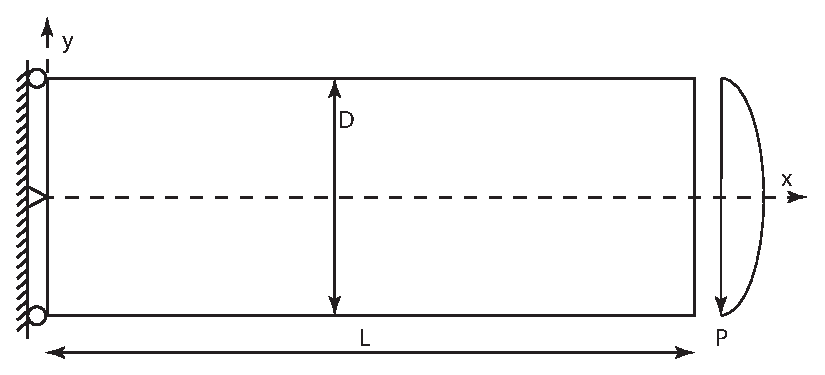
\includegraphics{isogeometric_sbfem/images/cantilever_beam_geo_bc.eps}}
        \caption{ Cantilever beam: Geometry and boundary conditions.}
        \label{fig:cantilever_beam_geo_bc}
    \end{figure}

The geometry is: length $L=8m$, height $D=4m$.
The material properties are: Young’s modulus $E$ = $3 \times 10^7 N/m^2$ , Poisson’s ratio $ν=0.25$.
The parabolic shear force is $P$ = $250 N$.
The exact solutions for the displacements are given by \cite{Aug2008}:
    \begin{equation}
        \begin{aligned}
            u(x,y) &= 
                \frac{Py}{6 \mean{E} I}
                \left[
                    \left(
                        6L-3x
                    \right)x
                    +\left(
                        2+ \mean{v}
                    \right)\left(
                        y^2-\frac{D^2}{4}
                    \right)
                \right]
            \\
            v(x,y) &=  
                -\frac{P}{6 \mean{E} I}
                \left[
                    3 \mean{v} y^2 \left(
                        L-x
                    \right)+
                    \left(
                        4+5 \mean{v}
                    \right)\frac{D^2x}{4}+
                    \left(
                        3L-x
                    \right)x^2
                \right]        
        \end{aligned}
    \label{eq:cantilever_beam_displacement_solution}
    \end{equation}

where $I=D^3/12$ is the moment of inertia, $\mean{E}=E$, $\mean{v}=v$ and $\mean{E}=E/(1-v^2)$, $\mean{v}=v/(1-v)$ for plane
    stress and plane strain condition respectively.
The stress $\sigma$ can be expressed as \cite{Aug2008}
    \begin{subequations}
    \begin{align}
        \sigma_{xx} &= \frac{P(L-x)y}{I} \\
        \sigma_{yy} &= 0 \\
        \tau_{xy} &= -\frac{P}{2I} \left[
            \frac{D^2}{4} - y^2
        \right]
    \end{align}
    \label{eq:cantilever_beam_stress_solution}
    \end{subequations}

The strain energy can be derived from eq.~\ref{eq:cantilever_beam_stress_solution} and eq.~\ref{eq:cantilever_beam_displacement_solution} as
    \begin{equation}
        \frac{1}{2} \left(
            \frac{D^3 L^3 P^2}{36EI^2} + 
            \frac{D^5LP^2(1+v)}{60EI^2}
        \right)
    \label{eq:cantilever_beam_energy_solution}
    \end{equation}

\paragraph{}
In this example, rigid body motion is constrained by fixing 3 DOF on the left edge of the beam.
$u_x=0$ for points at $(0,-D/2)$ and $(0,D/2)$ and $u_y =0$ for point at $(0,0)$.
Stress from analytical solution in eq.~\ref{eq:cantilever_beam_stress_solution} are applied on the boundary.

\paragraph{}
From the description in \ref{subsection:surface_traction}, the expression of the surface traction must be transformed into
    NURBS-like representation before the stress can be applied on the nodes.
Although least square is introduced to solve for the ``control stress'' $\Phi_c$, the control points that describe a second
    order function as surface traction in this example can be solved mathematically.
Assume the knot vector is evenly spaced and the shape function is in second order, i.e. knot vector $K=[0,0,0,1,1,1]$.
Weight vector will be uniform because only the straight line is being interpolated, i.e. weight vector $w=[1,1,1]$.
Three basis function used in B-Spline will be
    \begin{equation}
    \begin{aligned}
        N_1 & = (1-u)^2 \\
        N_2 & = 2u(1-u) \\
        N_3 & = u^2
    \end{aligned}
    \end{equation}

With the given targeted parabola as $y=ax^2+bx+c,x \in [0,1]$, the generalized control points for the NURBS curve will be
    \begin{equation}
        P= \begin{bmatrix}
            P_x \\
            P_y
        \end{bmatrix} = \begin{bmatrix}
            0 & m & 1 \\
            c & n & a+b+c
        \end{bmatrix}
    \end{equation}

where $m$ and $n$ are unknowns for the second control point.
B-spline curve $C=[N][[P]$ then can be expressed as in parametric form as
    \begin{equation}
        \left\{
        \begin{aligned}
            x &= 2u(1-u)m + u^2 \\
            y &= c(1-u)^2 + 2u(1-u)n + (a+b+c)u^2
        \end{aligned}
        \right.
    \label{eq:parabola_fitting_parametric}
    \end{equation}

After substituting eq.~\ref{eq:parabola_fitting_parametric} into $y=ax^2+bx+c$, we then have the system of equations as
    \begin{equation}
        \begin{bmatrix}
            0 \\
            0 \\
            2c - 2n +a +b \\
            2n - 2c \\
            c
        \end{bmatrix} = 
        \begin{bmatrix}
            4am^2-4am+a \\
            -8am^2 + 4am \\
            4am^2 -2bm +b \\
            2bm \\
            c
        \end{bmatrix}
    \end{equation}

$m$ and $n$ then can be solved as
    \begin{equation}
        \left\{
        \begin{aligned}
            m &= \frac{1}{2} \\
            n &= \frac{b+2c}{2}
        \end{aligned}
        \right.
    \end{equation}

\paragraph{}
The numerical convergence of the relative error in the displacement norm and the relative error in the energy norm are
    shown in fig.~\ref{fig:cantilever_beam_convergence} for various order of NURBS basis functions with refinement.
Fig.~\ref{fig:cantilever_beam_convergence} also shows the error in the displacement norm when quadratic Lagrange shape
    functions are used along each edge within the scaled boundary formulation.
It can be observed that NURBS basis functions yield superior accuracy when compared to Lagrange basis functions of the
    same order.
It is seen that as the order of the shape functions is increased, the error decreases while the convergence rate increases.

\begin{figure}
    \begin{subfigure}[b]{1\linewidth}
        \centering
        \scalebox{0.7}{
            % This file was created by matlab2tikz v0.4.6 running on MATLAB 8.2.
% Copyright (c) 2008--2014, Nico Schlömer <nico.schloemer@gmail.com>
% All rights reserved.
% Minimal pgfplots version: 1.3
% 
% The latest updates can be retrieved from
%   http://www.mathworks.com/matlabcentral/fileexchange/22022-matlab2tikz
% where you can also make suggestions and rate matlab2tikz.
% 
\begin{tikzpicture}

\begin{axis}[%
width=4.52083333333333in,
height=3.5146875in,
scale only axis,
xmode=log,
xmin=10,
xmax=1000,
xminorticks=true,
xlabel={Total DOF},
ymode=log,
ymin=1e-05,
ymax=1,
yminorticks=true,
ylabel={Error},
title={l2l Displacement  Error},
legend style={draw=black,fill=white,legend cell align=left}
]
\addplot [color=blue,solid,mark=square,mark options={solid}]
  table[row sep=crcr]{
20	0.223473837	\\
40	0.0493	\\
80	0.011281049	\\
160	0.00266076	\\
};
\addlegendentry{1st order};

\addplot [color=black!50!green,solid,mark=o,mark options={solid}]
  table[row sep=crcr]{
20	0.067810872	\\
40	0.003190002	\\
80	0.000250473	\\
160	2.27e-05	\\
};
\addlegendentry{2nd order};

\addplot [color=red,solid,mark=+,mark options={solid}]
  table[row sep=crcr]{
20	0.0713	\\
40	0.00707	\\
80	0.000688	\\
160	8.85e-05	\\
};
\addlegendentry{LNGL 2nd order};

\end{axis}
\end{tikzpicture}%
        }
        % \label{fig:cantilever_beam_displacement_convergence}
        \caption{the relative error in displacement norm $(L^2)$}
    \end{subfigure}
    
    \begin{subfigure}[b]{1\linewidth}
        \centering
        \scalebox{0.7}{
            % This file was created by matlab2tikz v0.4.6 running on MATLAB 8.2.
% Copyright (c) 2008--2014, Nico Schlömer <nico.schloemer@gmail.com>
% All rights reserved.
% Minimal pgfplots version: 1.3
% 
% The latest updates can be retrieved from
%   http://www.mathworks.com/matlabcentral/fileexchange/22022-matlab2tikz
% where you can also make suggestions and rate matlab2tikz.
% 
\begin{tikzpicture}

\begin{axis}[%
width=4.52083333333333in,
height=3.5146875in,
scale only axis,
xmode=log,
xmin=10,
xmax=1000,
xminorticks=true,
xlabel={Total DOF},
ymode=log,
ymin=0.001,
ymax=1,
yminorticks=true,
ylabel={Error},
title={l2l Strain Energy  Error},
legend style={draw=black,fill=white,legend cell align=left}
]
\addplot [color=blue,solid,mark=square,mark options={solid}]
  table[row sep=crcr]{
20	0.701427116670007	\\
40	0.417133072292284	\\
80	0.228254244210267	\\
160	0.119582607431014	\\
};
\addlegendentry{1st order};

\addplot [color=black!50!green,solid,mark=o,mark options={solid}]
  table[row sep=crcr]{
20	0.180496573374677	\\
40	0.02575787258296	\\
80	0.0046690470119715	\\
160	0.0010295630140987	\\
};
\addlegendentry{2nd order};

\addplot [color=red,solid,mark=+,mark options={solid}]
  table[row sep=crcr]{
20	0.304275389	\\
40	0.065	\\
80	0.014502273	\\
160	0.003385053	\\
};
\addlegendentry{LNGL 2nd order};

\end{axis}
\end{tikzpicture}%
        }
        % \label{fig:cantilever_beam_energy_convergence}
        \caption{the relative error in the energy norm}
    \end{subfigure}
\label{fig:cantilever_beam_convergence}
\caption{Bending of thick cantilever beam: Convergence results}
\end{figure}
\pagebreak
\section{Conclusions}    % chapter 3
% %!TEX root = ../thesis.tex
\chapter{Quad-tree mesh in 2D analysis}

\section{Introduction}
\paragraph{}
The main objective of this chapter is to introduce a way that can utilize the engineering design available in CAD or other popular commercial softwares for 2D case.
The data format that used in almost all engineering design softwares that can represent the geometry exactly is IGES file.
It will be used as a bridge between design and numerical analysis.

\paragraph{}
After the NURBS represented exact geometry has been extracted from the IGES file, a quad-tree mesh generation algorithm described in \ref{qt_sc:quadtree} will be adopted to generate high quality mesh.
Either the NURBS basis functions or the traditional shape function can be used as the shape function of the SBFEM solver.
% We further extend the method to problems with singularities within the framework of linear elastic fracture mechanics.
The proposed method enhances the conventional SBFEM and the salient features of the method are:
    \begin{itemize}
        \item No human effort need to generate the mesh
        \item Exact geometry will be retain
        \item High quality mesh from the quad-tree algorithm
    \end{itemize}
\pagebreak

\section{CAD output in 2D}
\label{qt_sc:iges}
\paragraph{}
IGES\cite{IGES1983} files are used as the bridge between engineering design and numerical analysis.
As a standard file format in engineering design industry, it is supported by almost all design softwares all over the world.
Consequently, by utilizing it we are able to minimize the human effort on mesh generation.

\subsection{Parse geometry in IGES file}
\paragraph{}
The IGES file (explained in detail in \ref{lr_sc:iges}) provides all information that describe the input geometry.
Abstract structure of the IGES file that describe a 2D geometry can be regarded as a simple curve-surface structure.
In other words, it defines the input geometry as certain number of surfaces with different colors.
Different colors represented different material properties in engineering practice.
Each surface contains a list of curve index which is corresponding to the curve information described in IGES file.

\paragraph{}
When IGES file is feed into the programme, each line in the directory entry will be parsed entity by entity.
Parameter in directory entry describe the type and reference to other useful values for the entity.
An entity may reference to one or many entities in directory entry.
Detail of the specification of each entity is explained in \cite{Nasr2007} in detail.

%=====================================================================================================================%
\subsection{Output to mesh generator}
\paragraph{}
The output file that the mesh generator read in will be a shorter summary of the input geometry.
Boundary representation will be kept as the data structure to describe the input geometry.
However, some fields apart from curve and surface will be added.
In the output file, geometry description will be organized as key points, polylines and surfaces.
The key points define the coordinate of all points and polylines are used to represented all curves including NURBS curves for simplification.
NURBS curves can be used directly by the mesh generator as well in \ref{qt_sc:nurbs} but it is found the computational cost in calculation of distance between points to NURBS curves surpass the merits of using it directly.
The exact geometry can be retained by projected the nodes on the boundary back to the origin NURBS curves at the end.

\paragraph{}
Represent a straight line with polyline will not be a problem, first and the last points will be enough to exact representation.
However, that is not the case for curves where curvature is not always zero.
Although using more points must increase the quality of polyline representation, computational cost in the mesh generation when calculating the distance increases at the same time.
Yet, selecting few points that result in a bad polyline representation leads to a poor quality mesh.
Elements may be twisted after the nodes on the boundary are projected to the origin curves.
As a consequence, a quantified index that can control the number and the position of the vertices on the polyline is necessary.

%=====================================================================================================================%
\subsection{Discretization of circular arc}
\paragraph{}
Chord ratio can be a good indicator for circular arc.
The arc length to chord length ratio $\frac{a}{L}$ illustrated in fig.~\ref{qt_fig:iges_chord_ratio} can be expressed in angle $\alpha$ as:
    \begin{equation}
        \frac{a}{L} = \frac{
            \sqrt{2-2\cos\alpha}
        }{\alpha}
        = \frac{
            2\sin\frac{\alpha}{2}
        }{\alpha}
    \end{equation}

The maximum angle $\alpha$ satisfy arc length to chord length ratio $\frac{a}{L} > 1-\epsilon$ with $
    \sin\frac{\alpha}{2} = 1 - \frac{x^3}{6} + O(x^7)
$ can be derived as:
    \begin{equation}
        \alpha < \sqrt{24 \epsilon}
    \end{equation}

    \begin{figure}[h!]
        \centering
        \scalebox{1.2}{
            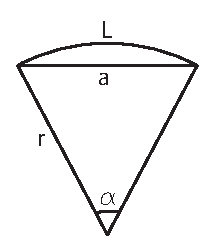
\includegraphics{quadtree/images/iges_chord_ratio.eps}
        }
        \caption{Chord length for circular arc}
        \label{qt_fig:iges_chord_ratio}
    \end{figure}

%=====================================================================================================================%
\subsection{Discretization of NURBS curves}
\paragraph{}
For NURBS curve there is no closed form chord ratio that can be utilized.
However, similar idea can be applied numerically.
The NURBS curves are first divided into serval smaller ones based on the knot vector.  % may be explained in detail
Since the order of each sub-divided NURBS curve used in engineering softwares are predominantly lower or equal to three, the sub-curves then can be divided into two classes, convex curves or concave curve with an inflection point as shown in fig.~\ref{qt_fig:iges_chord_ratio_nurbs}.
    \begin{figure}
        \begin{subfigure}[b]{0.5\linewidth}
            \centering
            \scalebox{0.5}{
                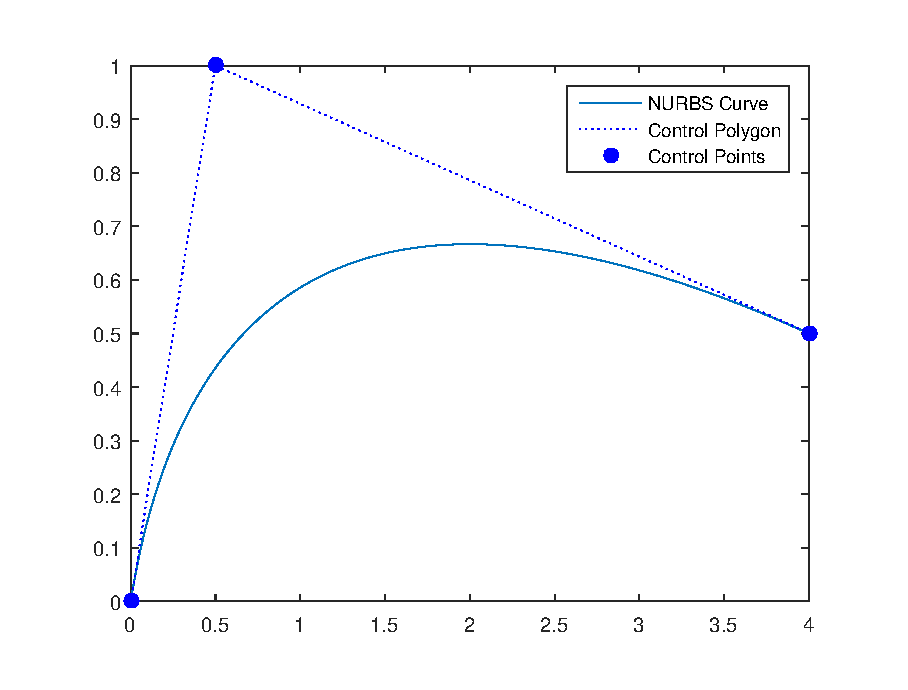
\includegraphics{quadtree/images/iges_chord_ratio_nurbs_convex.eps}
            }
            \caption{Convex}
        \end{subfigure}
        \begin{subfigure}[b]{0.5\linewidth}
            \centering
            \scalebox{0.5}{
                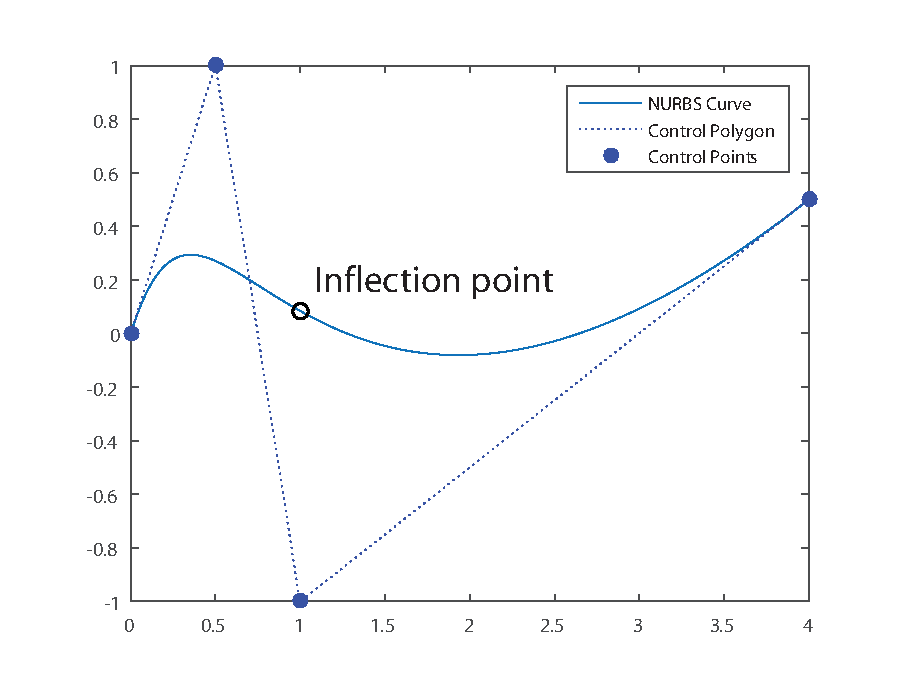
\includegraphics{quadtree/images/iges_chord_ratio_nurbs_concave.eps}
            }
            \caption{Concave with an inflection point}
        \end{subfigure}
    \caption{Type of sub-devided NURBS curves: convex and concave with an inflection point}
    \label{qt_fig:iges_chord_ratio_nurbs}
    \end{figure}

In order to determine the target NURBS curve is convex or concave, a cross product to assess whether the control net will be conducted.
Assuming the target sub-divided NURBS curve is cubic, there will be four control points $P_1,P_2,P_3$ and $P_4$.
If signs of $cross(\overrightarrow{P_1P_2},\overrightarrow{P_2P_3})$ and $cross(\overrightarrow{P_1P_2},\overrightarrow{P_2P_3})$ are the same, then the curve is convex. Otherwise it will be concave.

%=====================================================================================================================%
\subsubsection{Convex curves}
\label{qt_ssc:convex_curves}
\paragraph{}
Start with the simple case, in the situation illustrated in fig.~\ref{qt_fig:iges_chord_split_convex_sum} where line $C(u_0)C(u_n)$ and the NURBS curve form a convex set, we are looking for a point $C(u_m)$ on the curve so that $C'(u_m)$ is parallel to $\overrightarrow{C(u_0)C(u_n)}$
    \begin{figure}[h!]
        \centering
        \scalebox{0.8}{
            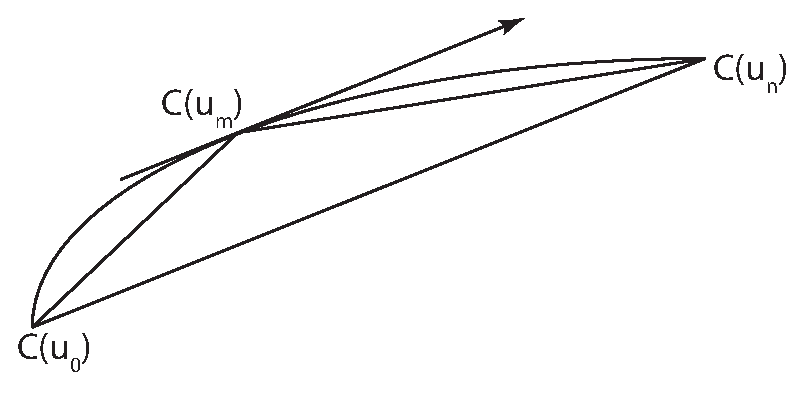
\includegraphics{quadtree/images/iges_chord_split_convex_sum.eps}
        }
        \caption{Discretization for convex NURBS curve}
        \label{qt_fig:iges_chord_split_convex_sum}
    \end{figure}

The target is then split one NURBS curve segment into two.
If any arc length to chord length ratio of these two ratio is below the tolerance given, the splitting will be processed recursively.
Based on the properties of the convex set, there is one and only one parameter $u_m$ that satisfy the condition.
As a consequence, numerical method such as Newton's method can be adopted to find it.
For a given $u_n$, the next iteration will be:
    \begin{equation}
        u_{n_{new}} =  u_n - \frac{f(u_n)}{f'(u_n)}
    \end{equation}

where 
    \begin{equation}
        f(u) = C'(u) \begin{bmatrix}
            - C_y(u_n) + C_y(u_0) \\
            C_x(u_n) - C_x(u_0)
        \end{bmatrix}
    \end{equation}


%=====================================================================================================================%
\subsubsection{Concave curves}
\paragraph{}
As can be seen in fig.~\ref{qt_fig:iges_chord_ratio_nurbs}, the extracted cubic NURBS curve will have no more than one inflection point.
The reason for that is because the target function is cubic and hence the second derivative of it will be in first order.
Consequently, numerical method such as Newton's method can be used to find this unique point.
After that, the curve can be divided into two convex ones and algorithms introduced in \ref{qt_ssc:convex_curves} can be used separately.
The Newton's iteration can be written as
    \begin{equation}
        u_{n_{new}} = u_n - \frac{f(u_n)}{f'(u_n)}
    \end{equation}

where
    \begin{equation}
        f(u) = C''(u)
    \end{equation}

%=====================================================================================================================%
\subsubsection{Calculation of the arc length}
\paragraph{}
The arc length of the NURBS curve defined on $u \in [u_0, u_1]$ can be expressed as
    \begin{equation}
        L = \int_{u_0} ^{u_1} \sqrt{C_x^2(u) + C_y^2(u)} du
    \end{equation}

The integration can be solved by the help of the numerical integration quadrature described in \ref{iso_subsection:numerical_integration} as:
    \begin{equation}
        L = \sum_{i=0}^n a_i \sqrt{C_x^2(u_i) + C_y^2(u_i)}
    \end{equation}

% \begin{algorithm}
% \caption{Discretization of a nurbs curve}
% \begin{algorithmic}[1]
%     \Procedure{YourFunction}{$x$}
%     \State Do Something
%     \EndProcedure
% \end{algorithmic}
% \end{algorithm}

\section{Quad-tree structure}
\label{qt_sc:quadtree}
\paragraph{}
After the geometry information is exported from the IGES file, it can be feed into the quad-tree algorithm to generate mesh of the problem domain.
As an algorithm based on computational geometry, it require great amount of numerical operation and hence the result may be sensitive to the tolerance.
An absolute tolerance may not be able to handle problem with very large or small geometric size.
As a consequence, the first step is to normalize the geometry into a uniform space ($10\times10$ is used in this chapter).

\subsection{Background mesh}
\paragraph{}
Background mesh describes a mesh in the background. %fig
Its density is decided by the geometry.
This section will introduce the procedure to generate the background mesh.
\paragraph{}
First of all, we start with one square which is the root of the tree.
The size of it will be slightly larger than the normalized input geometry and it is selected as $16 \times 16$ in this chapter.
After that, the root square will be divided into millions (defined by resolution, defined as $2^{res} \times 2^{res}$) smaller ones like pixels in the image.
Then, $2^{s_{max}} \times 2^{s_{max}}$ ``pixels'' will be group into the first layer of the tree, or initial background mesh as shown in fig.~\ref{qdt_fig:qdt_initial_mesh}.
It is used to control the maximum allowable mesh size globally or separately for different material regions.

\begin{figure}[!ht]
    \centering
    \scalebox{0.8}{
        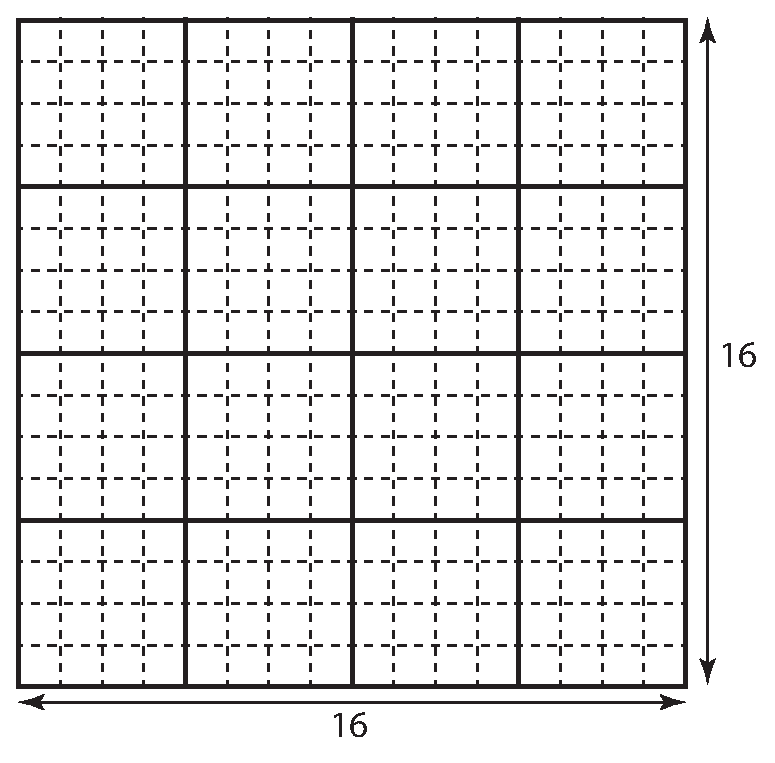
\includegraphics{quadtree/images/qdt_initial_mesh.eps}
    }
    \caption{An example of the background initial mesh: $16 \times 16$ square are divided into $2^4 \times 2^4$ pixels (dashed lines, $res=4$) and $2^2 \times 2^2$ pixels form the initial mesh (solid lines, $s_{max}=2$)}
    \label{qdt_fig:qdt_initial_mesh}
\end{figure}

\paragraph{}
% generating the initial mesh without balance
Criteria to decided whether each individual square in the initial mesh need to be refined or not is the seed points.
The curve will be uniformly discretized into a given number of seed points uniformly and the mesh will be refined until the number of the seed points within the square is less than the threshold.
However, finer mesh is expected at the region where geometry with high curvature appeared but the uniform discretization does not generate different number of points based on curvature.
It can be solved by treating each segment of the polylines as an individual curve when generating seed points.
Due to the fact that algorithm described in .~\ref{qdt_section:iges_output} guarantee the chord length to arc length ratio, polylines ought to have finer segments at the position where curvature is significant.

\paragraph{}
% only two intersections allowed
Although seed points provides a good guide on the mesh density, situations where high density mesh is required while few seed points appeared may happen as plotted in fig.~\ref{qdt_fig:qdt_seed_point_problem}.
The geometry limits the seed points due to the lack of curvature.
While, it is expected that the square element will be refined at least once as one layer of mesh may not be appropriate to formulate a thin shell structure. 
    \begin{figure}[!ht]
        \centering
        \scalebox{1}{
            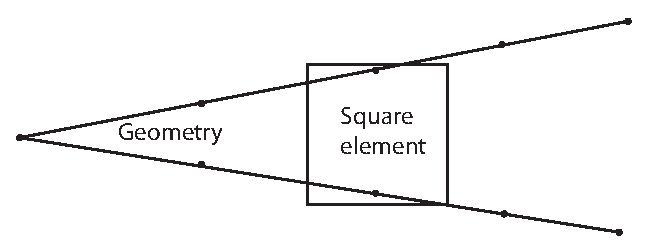
\includegraphics{quadtree/images/qdt_seed_points_problem}
        }
        \caption[Limitation of the seed points]{
            Limitation of the seed points: few seed points will be generated over a straight line and few seed points will be included in the square element which leads to unexpected behavior.
            \tikz\draw[black,fill=black] (0,0) circle (.7ex);
            stands for the seed points.
        }
        \label{qdt_fig:qdt_seed_point_problem}
    \end{figure}
As a result, another restriction will be adopted together with the seed points to prevent this kind of situation from happening.
Element with more than two unique intersections will be tagged to be refined no matter how many seed points it contains.
In numerical calculation, two points may be regarded as one if they are close enough to each others.
Normalization of the geometry described at the beginning of this section helps to define a meaningful tolerance to handle numerical error.



% balance the initial mesh
\paragraph{}
% balance in tree data structure
Self-balancing is adopted by most of the tree data structure such as AVL, B/B+, Red-black tree and so on.
Fig.~\ref{qdt_fig:tree_balance_avl} illustrates a self-balancing of an AVL tree.
Balancing by rotation is performed because difference in height of the leaf B and L is greater than the threshold.
    \begin{figure}
        \centering
        \scalebox{0.25}{
            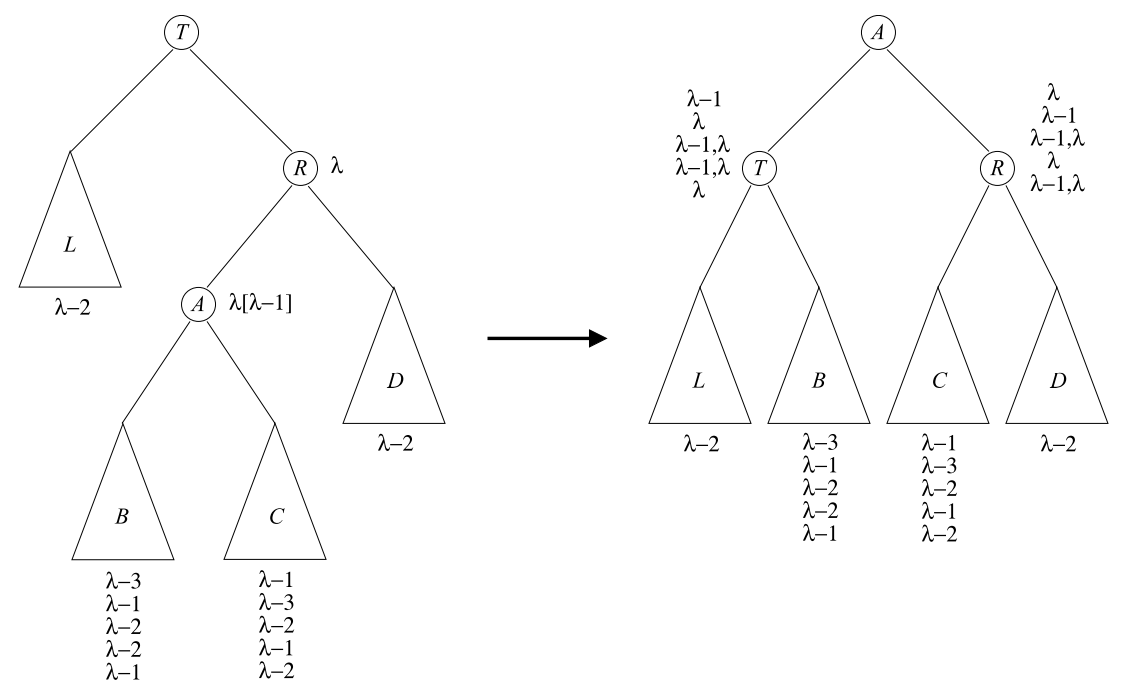
\includegraphics{quadtree/images/qdt_avl_balance.png}
        }
        \caption{Balance of the AVL tree \cite{Roura2013}}
        \label{qdt_fig:tree_balance_avl}
    \end{figure}

\paragraph{}
% balance in quadtree
Same idea is adopted in quadtree as well.
a refinement will be performed to achieve a balanced tree if the difference in the height of the leaf (Cell A and B in fig.~\ref{qdt_fig:tree_balance_quadtree} for example) is larger than one.
    \begin{figure}[!ht]
        \begin{subfigure}[b]{0.5\linewidth}
            \centering
            \scalebox{0.8}{
                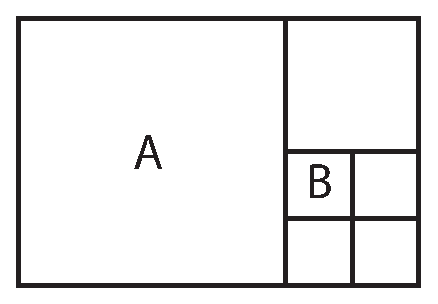
\includegraphics{quadtree/images/qdt_balance_before.eps}
            }
            \caption{Before balance operation}
        \end{subfigure}
        \begin{subfigure}[b]{0.5\linewidth}
            \centering
            \scalebox{0.8}{
                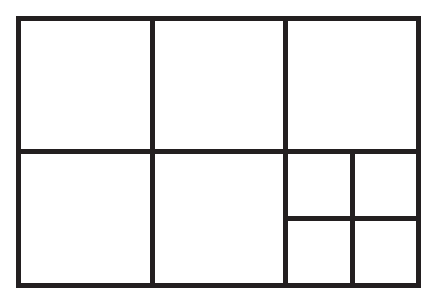
\includegraphics{quadtree/images/qdt_balance_after.eps}
            }
            \caption{After balance operation}
        \end{subfigure}
        \caption{Balance of quadtree: cell A is refined in order to balance the quadtree.}
        \label{qdt_fig:tree_balance_quadtree}
    \end{figure}

\paragraph{}
% reason behind balancing
The reason why balancing is predominately adopted in tree data structure lies in the guarantee of an $O\left(log(n)\right)$ time complexity for searching in any case.
Even thought computational cost on searching seems not to be significant during mesh generation using quadtree, a balanced tree provided some other attractive features that can be utilized in numerical analysis.
One of the advantages is to improve the mesh quality.
Any extremely small or large angle between the element and the scaling center may result in a bad quality mesh.
Chances are that these poor quality mesh may appear without self-balancing, fig.~\ref{qdt_fig:sbfem_adv_1} for an example.
    \begin{figure}[!ht]
        \centering
        \scalebox{1}{
            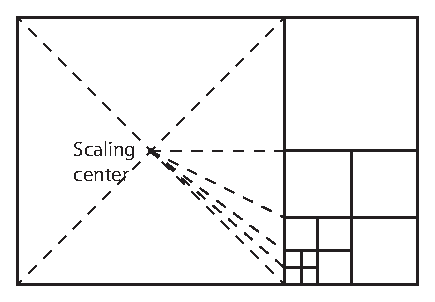
\includegraphics{quadtree/images/qdt_balance_sbfem_adv_1.eps}
        }
        \caption{Small angle between element and scaling center may reduce the mesh quality}
        \label{qdt_fig:sbfem_adv_1}
    \end{figure}

Another reason is to kept the pattern of the cells.
If the threshold of the self-balancing is set to one ($2:1$ ratio), only six kinds of cells will appear before the cutting as illustrated in fig.~\ref{qdt_fig:sbfem_adv_2}.
Thanks to the geometric similarity, local stiffness matrix can be calculated and scaled directly when same kind of the cell appears which significantly reduce the computational cost.
Hanging nodes in fig.~\ref{qdt_fig:sbfem_adv_2} can be a problem for traditional finite element to handle the displacement compatibility \cite{Tabarraei:2009:XFE} \cite{NME:NME3070} \cite{NME:NME2900} .
Solution including triangulation \cite{4037344} \cite{BERN1994384} \cite{ijeas251083} , using special shape function \cite{NME:NME1620120104} and other methods are available but special treatment is required.
As a comparison, SBFEM provides greater flexibility on the element, n-sides polygons with hanging nodes or curved edge can be treated natively.
    \begin{figure}[!ht]
        \centering
        \scalebox{1}{
            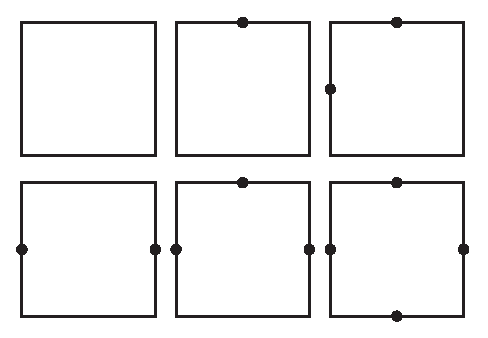
\includegraphics{quadtree/images/qdt_balance_sbfem_adv_2.eps}
        }
        \caption[Types of the cell in self-balancing quadtree]{
            Types of the cell when $2:1$ ratio is applied,
            \tikz\draw[black,fill=black] (0,0) circle (.7ex);
            stands for the hanging node
            }
        \label{qdt_fig:sbfem_adv_2}
    \end{figure}


\pagebreak


%=====================================================================================================================%
\subsection{Hard point treatment}
\paragraph{}
%introduction
Hard point is a kind of point in the geometry that must be meshed as a node or scaling center.
When more than two materials are involved, it is common to have some hard points to make sure the point shared by three material can be properly formulated as shown in fig.~\ref{qdt_fig:qdt_hard_point_demo}
    \begin{figure}[!ht]
        \begin{subfigure}[b]{0.5\linewidth}
            \centering
            \scalebox{0.8}{
                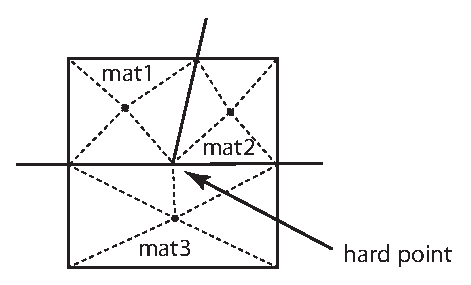
\includegraphics{quadtree/images/qdt_hard_point_demo.eps}
            }
        \caption{Hard point is meshed as node}
        \end{subfigure}
        \begin{subfigure}[b]{0.5\linewidth}
            \centering
            \scalebox{0.8}{
                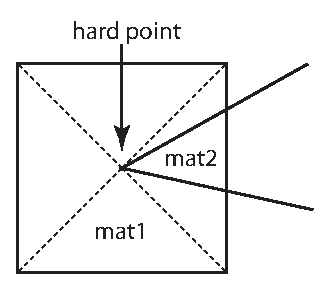
\includegraphics{quadtree/images/qdt_hard_point_demo_2.eps}
            }
        \caption{hard point is meshed as scaling center}
        \label{qdt_fig:qdt_hard_point_demo_sc}
        \end{subfigure}
        \caption[Example of a hard point]{Example of a hard point, elements around the point shared by three material must be properly divided into three.}
        \label{qdt_fig:qdt_hard_point_demo}
    \end{figure}
The difficulty in treating a hard point will be the position of itself in the background mesh.
The further it is away from the geometric center of the background mesh, the poorer the quality of mesh will be generated.
If the hard point in fig.~\ref{qdt_fig:qdt_hard_point_demo_sc} is located somewhere that is very close to the left boundary of the background mesh, the mesh for material one after cutting may be a quite elongated and twisted concave unit.
Besides, the requirement of the scaling center in the SBFEM can always be satisfied no matter where it is located in a convex polygon.
The opposite is true for a concave polygon, special treatment must be adopted to fullfil this requirement.
As a consequence, generally speaking, a convex mesh may always be preferred over a concave one and hard point can be the only source that will introduce concave polygons in most of the situation.
Although algorithm finding qualified scaling center in a concave polygon exists, the quality of the mesh may not be satisfactory even the scaling center is located on the vertex.


\paragraph{}
% make sure the hard point is close to the center of the background mesh
The first step to treat the hard point will be trying to locate the background mesh so that the hard point is close enough to its geometric center.
The ideal size of the background mesh shall ensure that only one hard point is in it and that no points from any other curves should be located in it.
As a consequence, the size of the containing square $box\_size$ is set to be one third of the distance to the nearest curves or half of the distance to the nearest hard point, whichever is smaller.
These parameter usually result in a valid and large enough background mesh that can treat the hard point easily. 
When building the background cell containing hard point in the algorithm, it will be implemented by have a considerably fine mesh within the range of the hard point and merge all cells in that range into one larger cell to be the background one.
Size of the ``considerably fine'' mesh $size\_field$ will be defined with the adjacent vertexes of the hard point as in eq.~\ref{qdt_eq:qdt_hard_point_size_field}
    \begin{equation}
        size\_field = \frac{box\_size}{
            2^{
                round(
                    \log(\frac{2 \pi}{ min(\alpha)})-1
                )
            }
        }
    \label{qdt_eq:qdt_hard_point_size_field}
    \end{equation}
where $\alpha$ is the minimal angle $min(\alpha_1, \alpha_2, \dots, \alpha_n)$ in fig.~\ref{qdt_fig:qdt_hard_point_setp_1}.
As is exponentially related to the minimal angle $\alpha$, the $size\_field$ may always be small enough to capture thin shell.
    \begin{figure}
        \centering
        \scalebox{0.5}{
            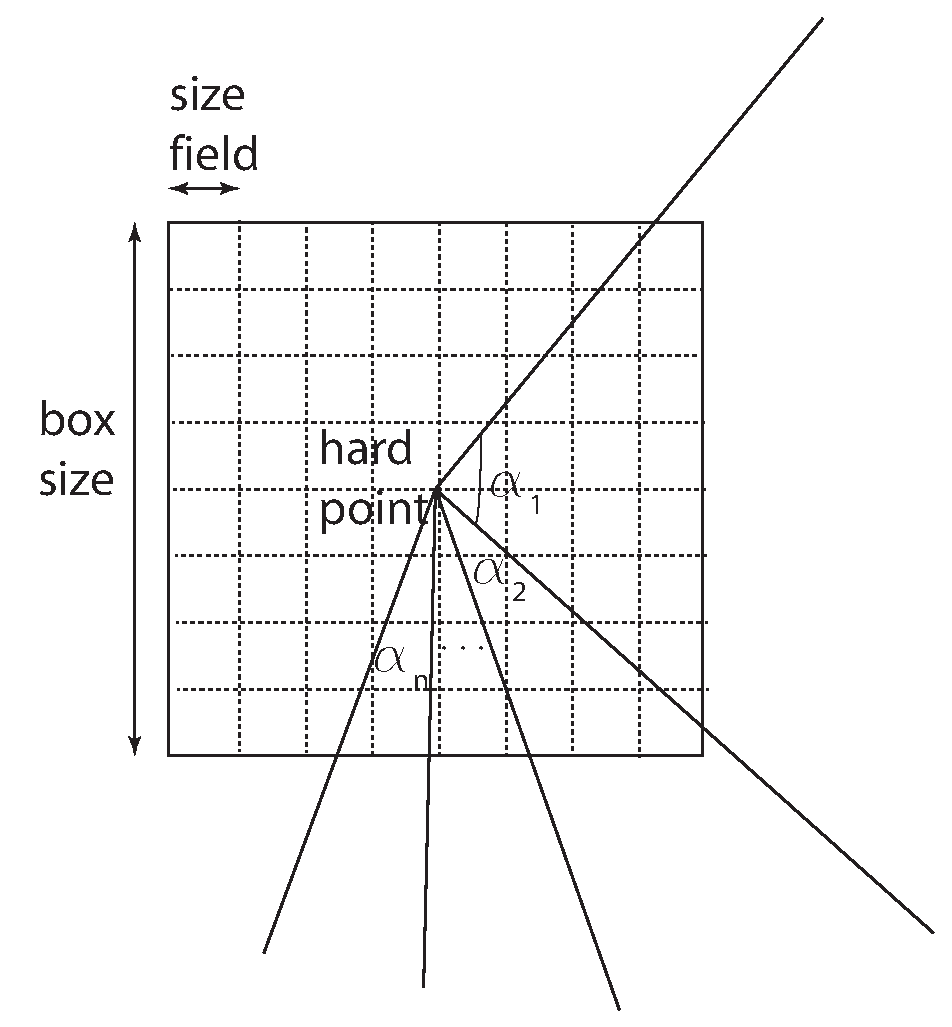
\includegraphics{quadtree/images/qdt_hard_point_step_1.eps}
        }
        \caption[Hard point treatment step 1]{Hard point treatment step1: find $box\_size$ and $size\_field$}
        \label{qdt_fig:qdt_hard_point_setp_1}
    \end{figure}

After the first step of the hard point treatment is done, the background cell shall have the following properties
    \begin{enumerate}
        \item Distance between hard point to geometric center of the background cell must be smaller than $\sqrt{2}size\_field$
        \item Element after cutting share the hard point as the node or it will be one element with scaling center located at the hard point
    \end{enumerate}
With these two properties, the cell can be cut by simply connecting the intersections with the hard point later.
\pagebreak


%=====================================================================================================================%
\subsection{Bucket sort algorithm}



\pagebreak
%=====================================================================================================================%
\subsection{Cutting with boundary}



\pagebreak
%=====================================================================================================================%
\subsection{Scaling center for concave elements}



\pagebreak
%=====================================================================================================================%
\subsection{Color the region}



\pagebreak

% \section{NURBS utilization}
% \label{qt_sc:nurbs}
% \input{quadtree/nurbs.tex}


\section{Numerical Examples}
\subsection{Cantilever beam}
\paragraph{}
A two-dimensional cantilever beam subjected to a parabolic shear load at the free end is examined as shown
in fig.~\ref{qdt_fig:ex_cantilever_beam_geo_bc}.
    \begin{figure}[h!]
    \centering
        \scalebox{0.8}{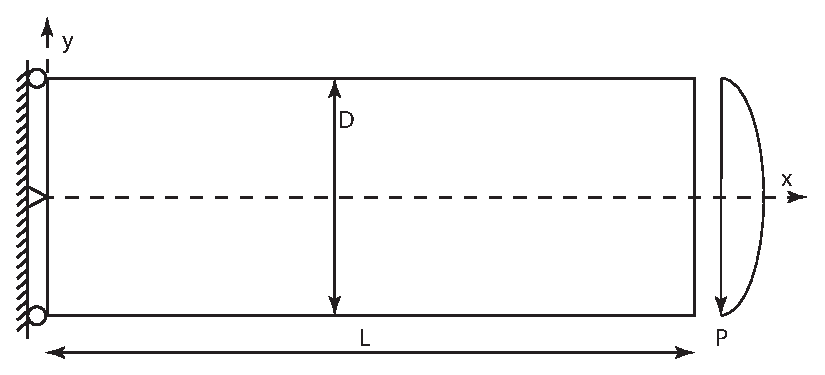
\includegraphics{isogeometric_sbfem/images/cantilever_beam_geo_bc.eps}}
        \caption{ Cantilever beam: Geometry and boundary conditions.}
        \label{qdt_fig:ex_cantilever_beam_geo_bc}
    \end{figure}

The geometry is: length $L=8m$, height $D=4m$.
The material properties are: Young’s modulus $E$ = $3 \times 10^7 N/m^2$ , Poisson’s ratio $ \nu =0.25$.
The parabolic shear force is $P = 250 N$.
The exact solutions for the displacements are given by \cite{Aug2008} as eq.~\ref{iso_eq:cantilever_beam_displacement_solution}.
where $I=D^3/12$ is the moment of inertia, $\mean{E}=E$, $\mean{\nu}=\nu$ and $\mean{E}=E/(1-\nu^2)$, $\mean{\nu}=nu/(1-nu)$ for plane stress and plane strain condition respectively.
The stress $\sigma$ can be expressed as \cite{Aug2008} as eq.~\ref{iso_eq:cantilever_beam_stress_solution}.
The strain energy can be derived from eq.~\ref{iso_eq:cantilever_beam_stress_solution} and eq.~\ref{iso_eq:cantilever_beam_displacement_solution} as eq.~\ref{iso_eq:cantilever_beam_energy_solution}.

\paragraph{}
In this example, rigid body motion is constrained by fixing 3 DOF on the left edge of the beam.
$u_x=0$ for points at $(0,-D/2)$ and $(0,D/2)$ and $u_y =0$ for point at $(0,0)$.
Stress from analytical solution in eq.~\ref{iso_eq:cantilever_beam_stress_solution} are applied on the boundary.

\paragraph{}
Due to the fact that the geometry of the cantilever beam can be described by four points and four straight lines, drawing in AutoCAD may not be necessary.
As a result, the input geometry is defined manually.
Generated background mesh, coloring and the final result with $res=32$, $s_{max}=16$ and $s_{min}=1$ are shown in fig.~\ref{qdt_fig:ex_cantilever_beam_background_mesh}, fig.~\ref{qdt_fig:ex_cantilever_beam_mesh_coloring} and fig.~\ref{qdt_fig:ex_cantilever_beam_mesh_final}.

    \begin{figure}
        \centering
        \scalebox{0.6}{
            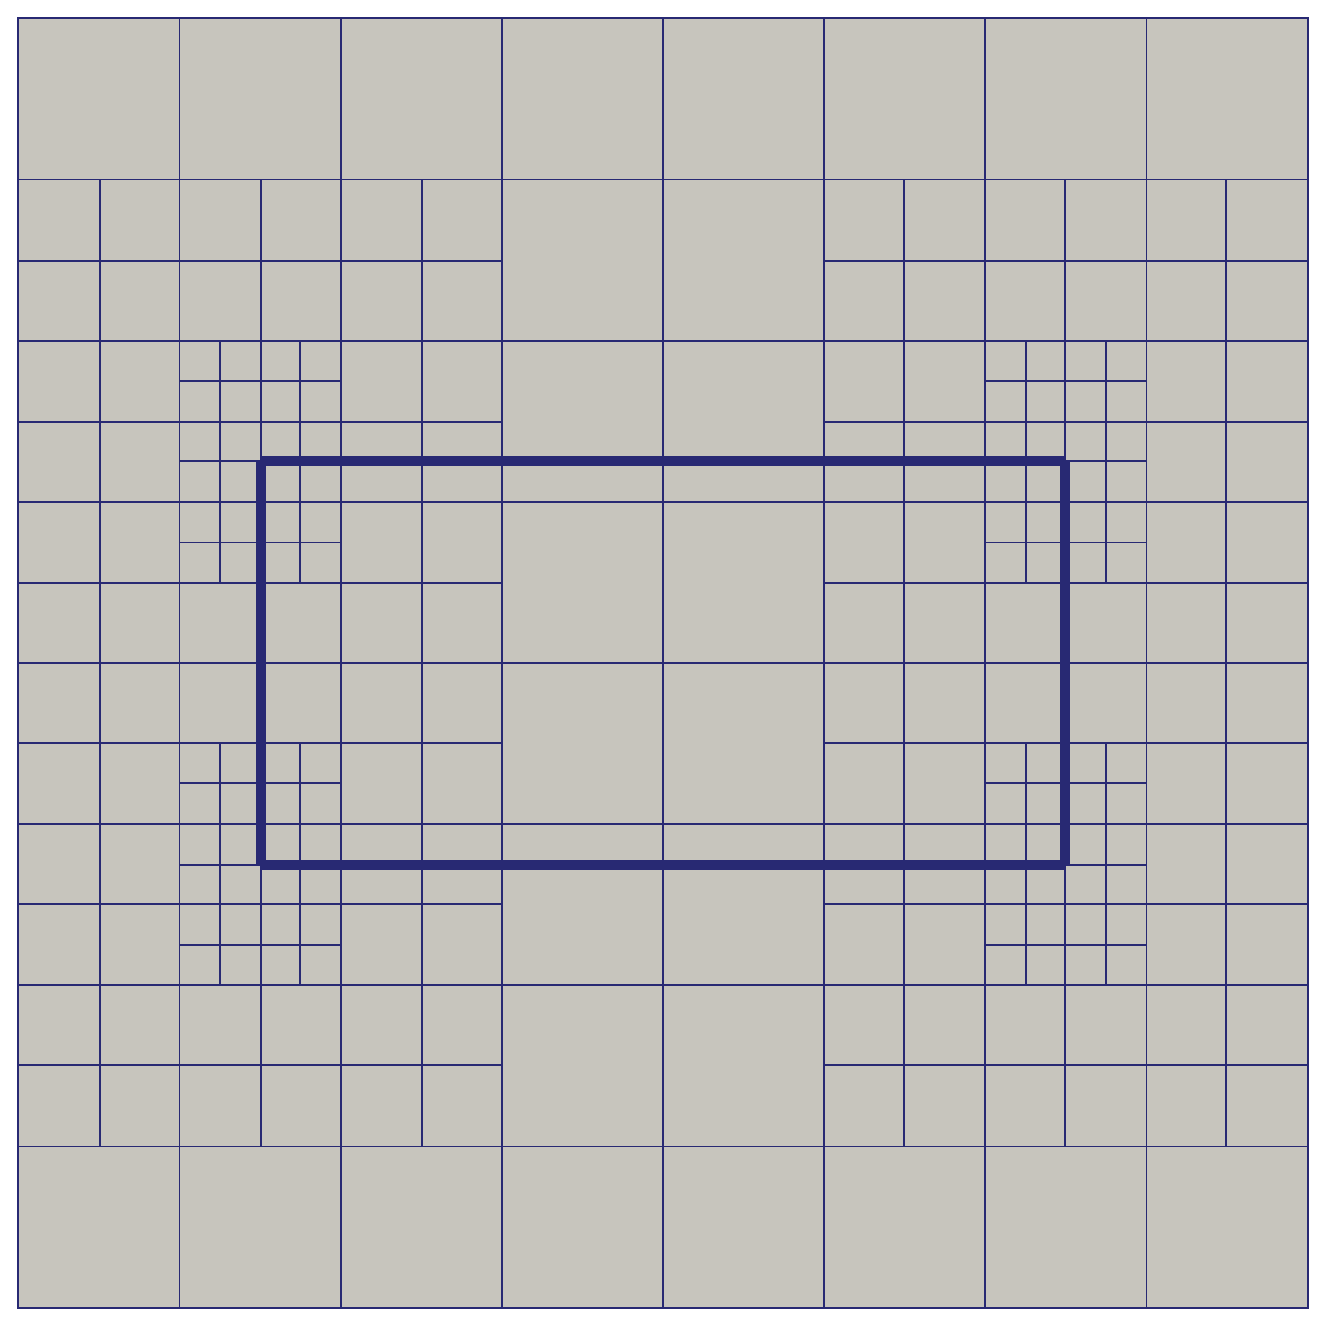
\includegraphics{quadtree/ex_images/cantilever_background_mesh.eps}
        }
        \caption[Background mesh of cantilever beam]{Background mesh of cantilever beam : Bold lines represents the input geometry}
        \label{qdt_fig:ex_cantilever_beam_background_mesh}
    \end{figure}

    \begin{figure}
        \centering
        \scalebox{0.6}{
            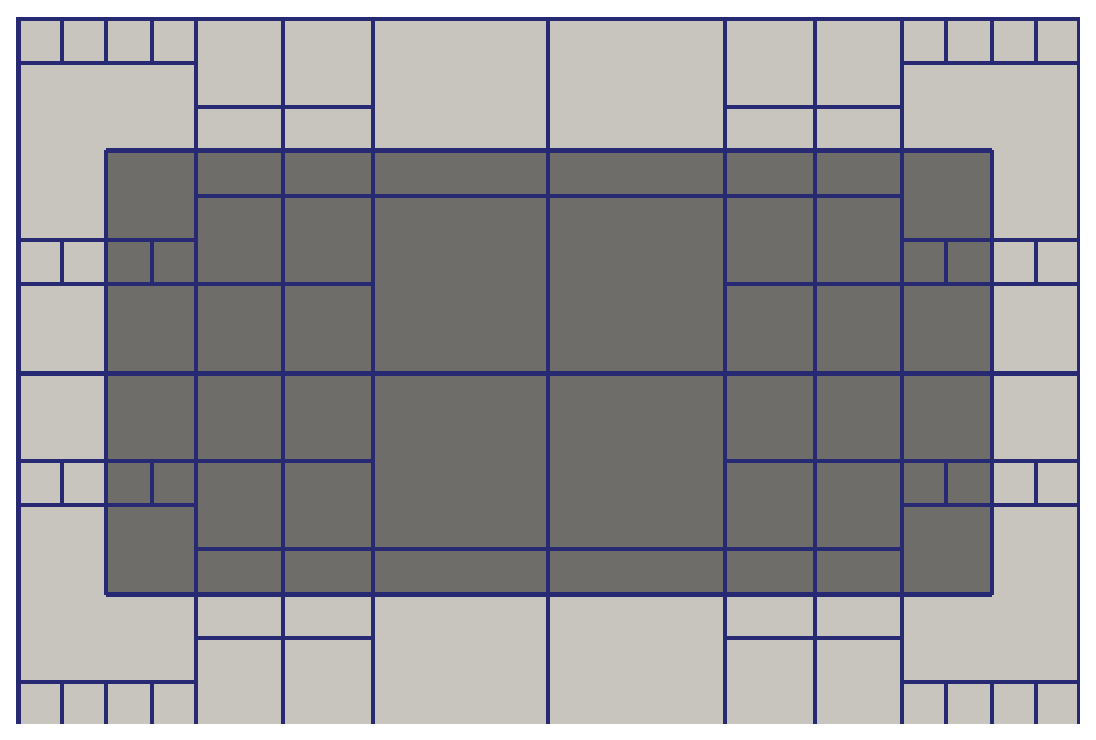
\includegraphics{quadtree/ex_images/cantilever_coloring.eps}
        }
        \caption[Mesh coloring of cantilever beam]{Mesh coloring of cantilever beam : Grey area represents the cantilever beam}
        \label{qdt_fig:ex_cantilever_beam_mesh_coloring}
    \end{figure}

    \begin{figure}
        \centering
        \scalebox{0.5}{
            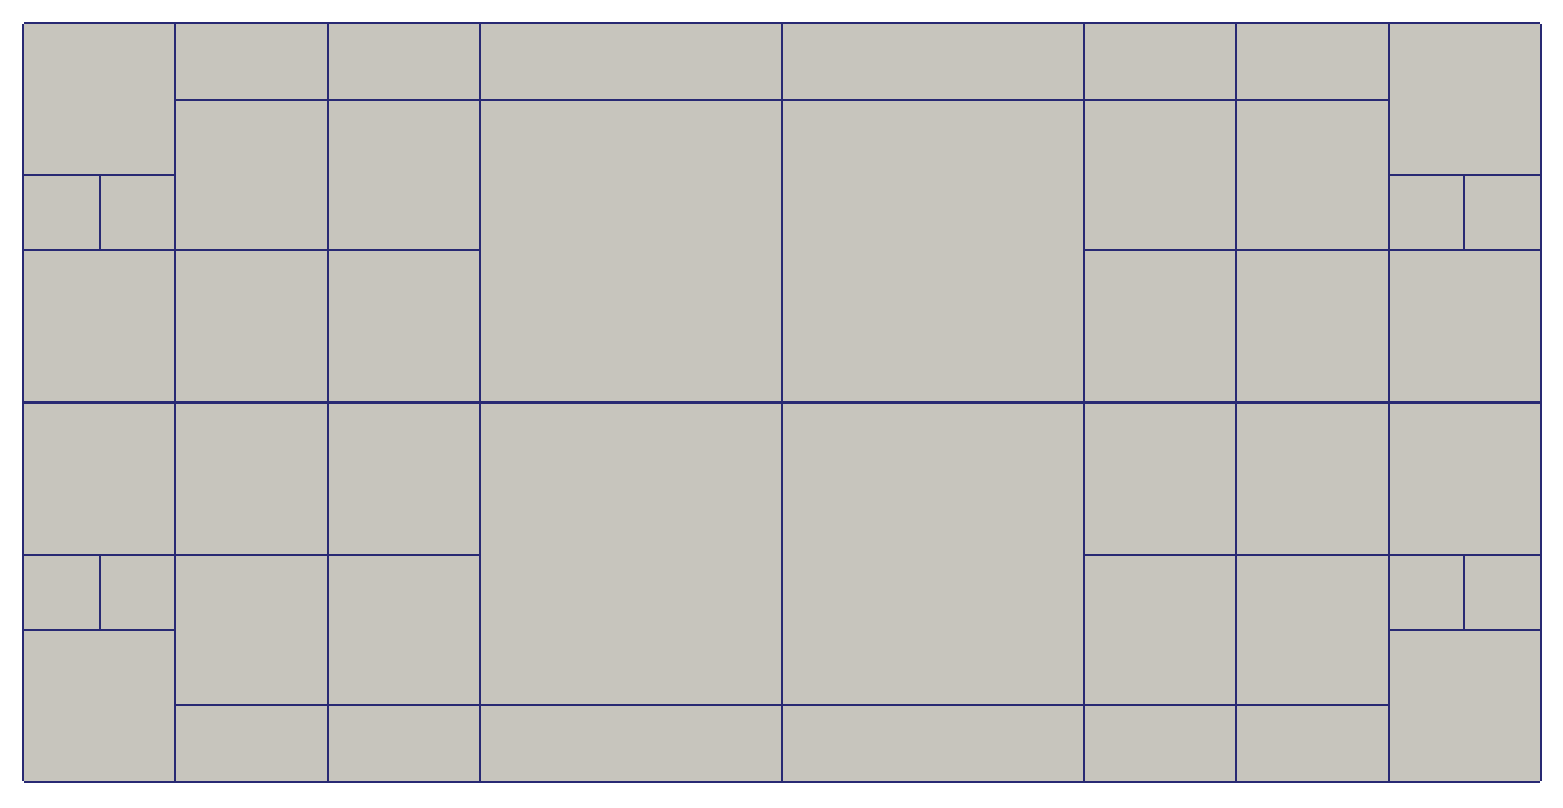
\includegraphics{quadtree/ex_images/cantilever_final_mesh.eps}
        }
        \caption[Final mesh of cantilever beam]{Final mesh of cantilever beam}
        \label{qdt_fig:ex_cantilever_beam_mesh_final}
    \end{figure}
% DOF err
% 146 - 0.019587 (32,16)
% 178 - 0.0082845 (32,2)
% 438 - 0.0027044 (64,2)
% 1658- 0.00066929 (128,2)
\paragraph{}
Mesh with different parameters are plotted in fig.~\ref{qdt_fig:ex_cantilever_mesh_all} and the convergence study is plotted in fig.~\ref{qdt_fig:ex_cantilever_mesh_conv}

    \begin{figure}[!ht]
        \begin{subfigure}[b]{1\linewidth}
            \centering
            \scalebox{0.4}{
                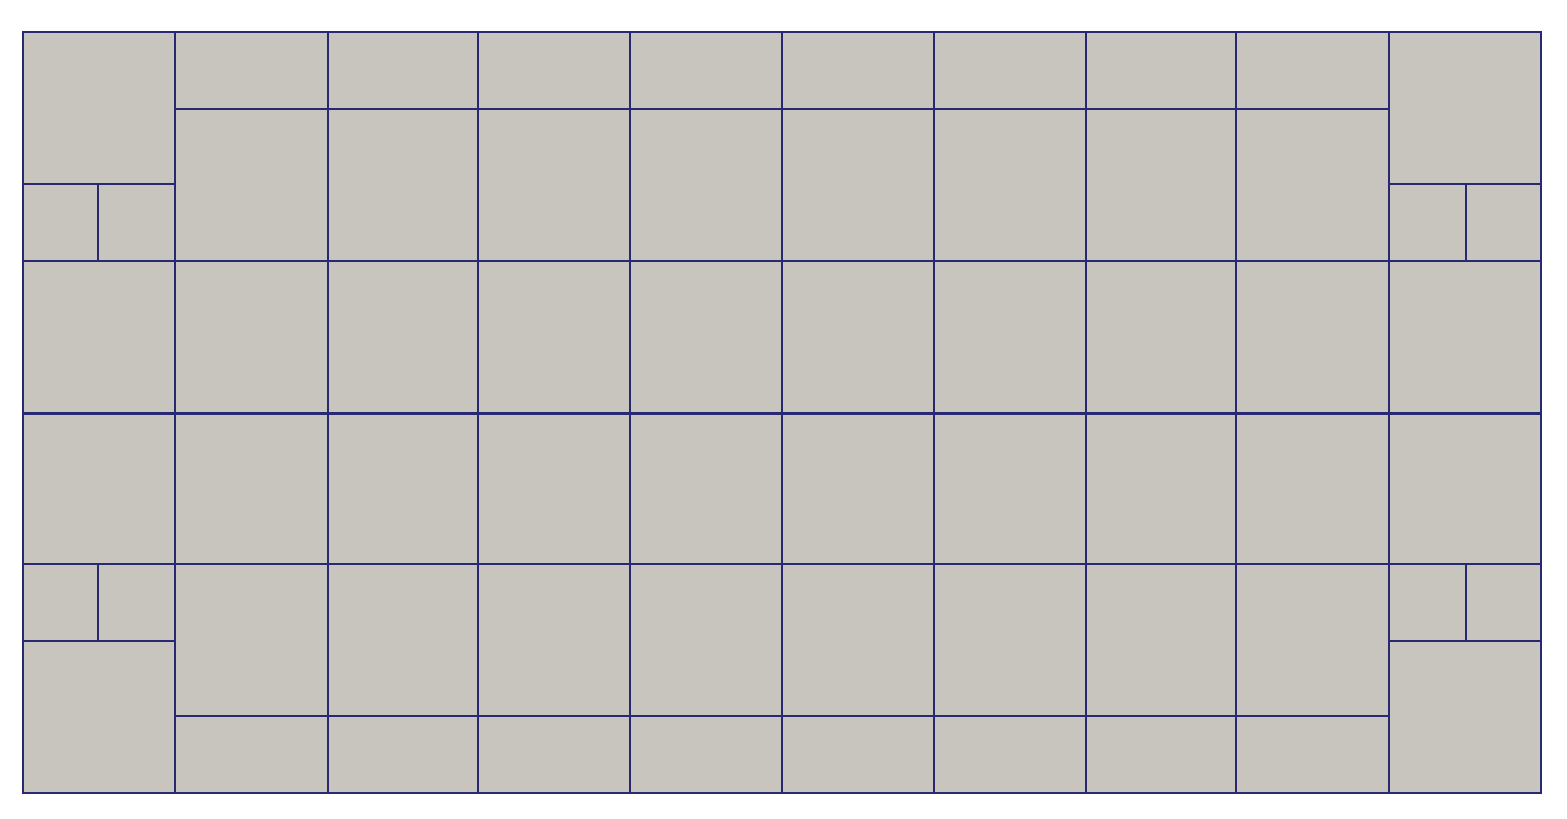
\includegraphics{quadtree/ex_images/qdt_cantilever_mesh_178.eps}
            }
            \caption{Mesh with $res=32$, $s_{max}=2$, 178 DOFs}
        \end{subfigure}
        \\
        \begin{subfigure}[b]{1\linewidth}
            \centering
            \scalebox{0.4}{
                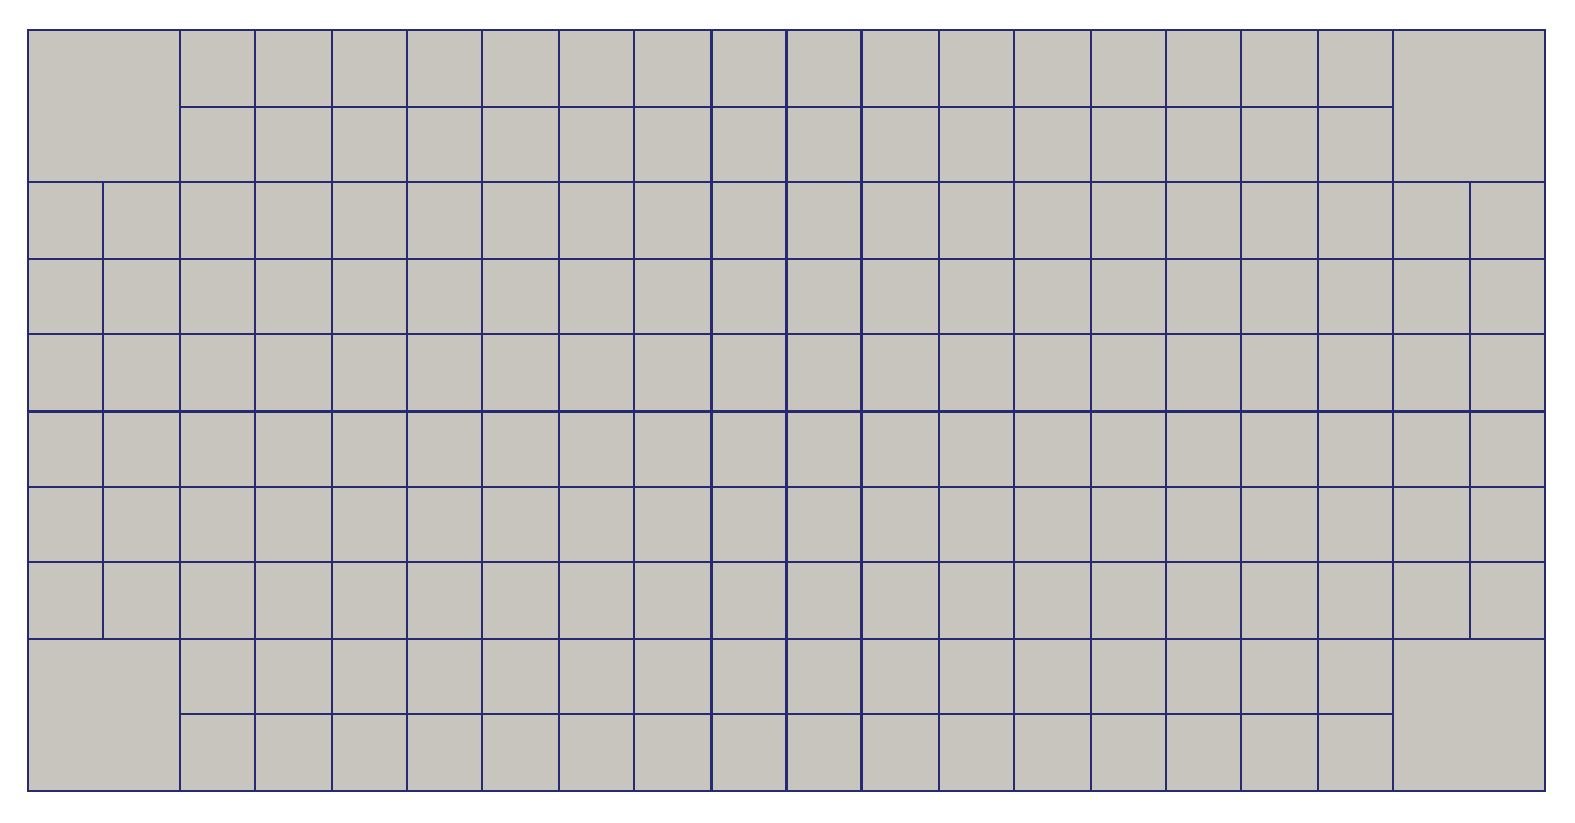
\includegraphics{quadtree/ex_images/qdt_cantilever_mesh_438.eps}
            }
            \caption{Mesh with $res=64$, $s_{max}=2$, 438 DOFs}
        \end{subfigure}
        \\
        \begin{subfigure}[b]{1\linewidth}
            \centering
            \scalebox{0.4}{
                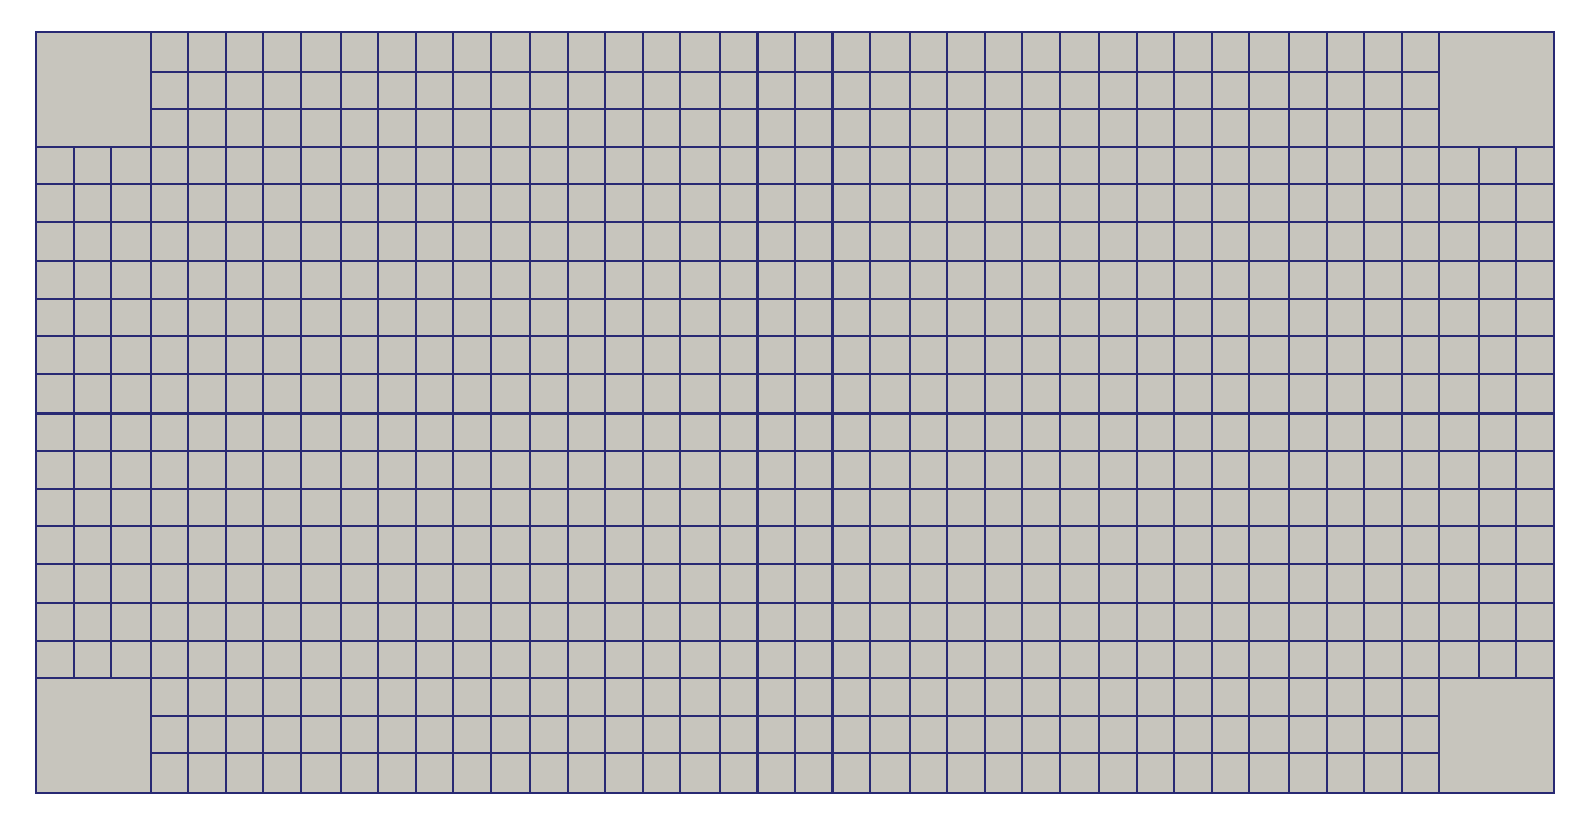
\includegraphics{quadtree/ex_images/qdt_cantilever_mesh_1658.eps}
            }
            \caption{Mesh with $res=128$, $s_{max}=2$, 1658 DOFs}
        \end{subfigure}
        \caption[Mesh of the cantilever beam]{Mesh of the cantilever beam}
        \label{qdt_fig:ex_cantilever_mesh_all}
    \end{figure}


    \begin{figure}[H]
        \centering
        \scalebox{0.75}{
            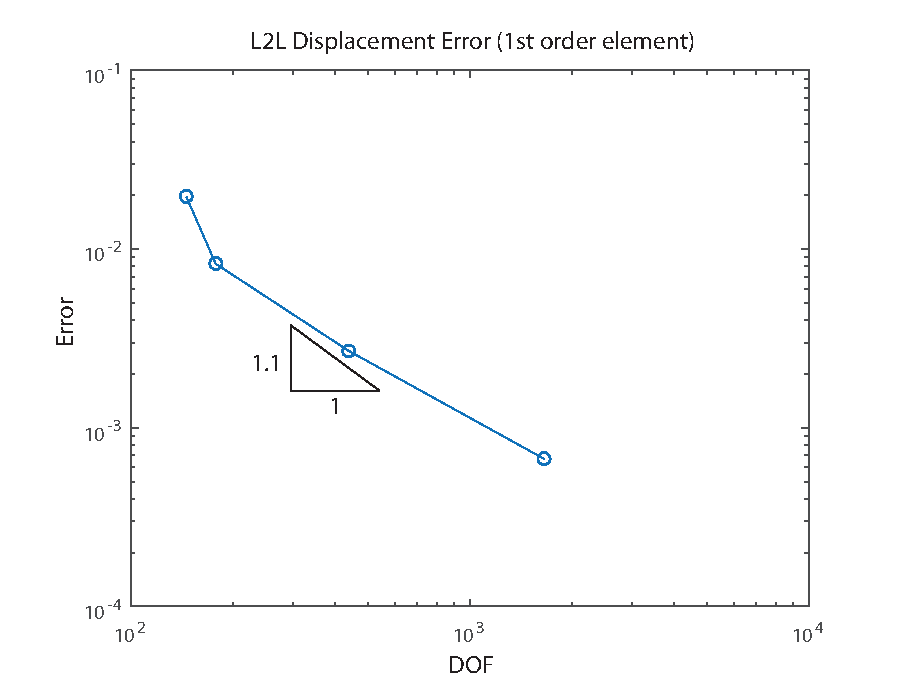
\includegraphics{quadtree/ex_images/qdt_cantilever_conv.eps}
        }
        \caption[Convergence of the cantilever beam]{Convergence of the cantilever beam}
        \label{qdt_fig:ex_cantilever_mesh_conv}
    \end{figure}

    
\pagebreak
\subsection{Infinite plate with a circular hole}
\paragraph{}
In this example, an infinite plate with a traction free hole under uniaxial tension $(\sigma = 1 N/m^2 )$ along x-axis (see Fig.~\ref{qdt_fig:ex_chole_geo_bc}) is considered.
$L$ is taken as $20$ and $r$ is $5$.
The material properties are: Young’s modulus $E = 100 N/m^2$ and Poisson’s ratio $\nu = 0.3$.
    \begin{figure}[H]
        \centering
        \scalebox{0.5}{
            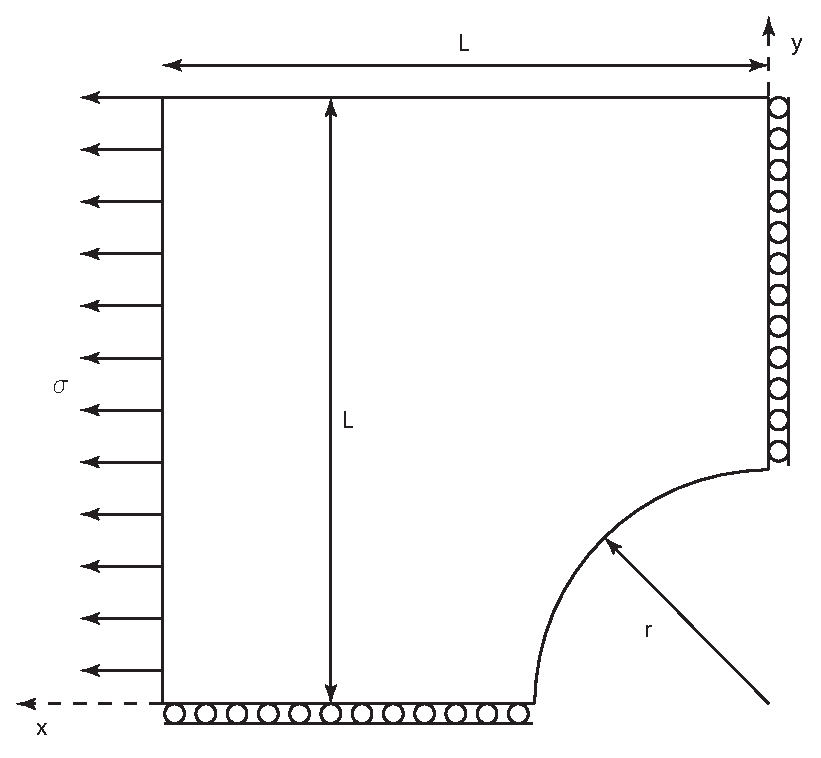
\includegraphics{quadtree/ex_images/qdt_chole_quat_geo_bc.eps}
        }
        \caption{ Infinite plate with a circular hole: geometry and boundary conditions}
        \label{qdt_fig:ex_chole_geo_bc}
    \end{figure}
%
The exact solution of the principal stresses in Cartesian coordinate $(r,\theta)$ is given by \cite{Sukumar2001} in Eq.~\ref{iso_eq:ex_chole_stress_sol}.
The closed form displacement in Cartesian coordinate is given in Eq.~\ref{iso_eq:ex_chole_disp_sol}.
\paragraph{}
Geometry of the example will be extracted from the iges file drawn in AutoCAD (Fig.~\ref{qdt_fig:ex_chole_cad}).
    \begin{figure}[H]
        \centering
        \scalebox{0.35}{
            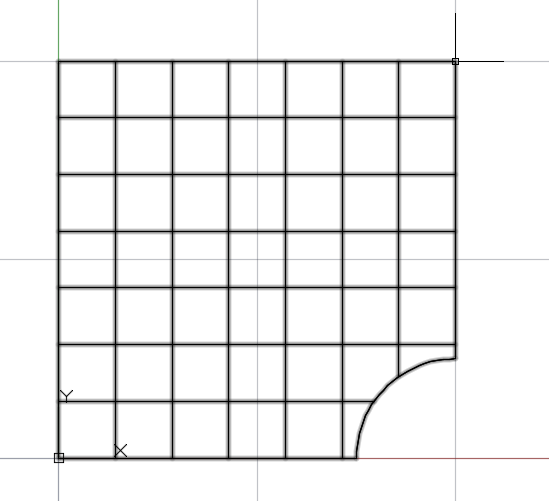
\includegraphics{quadtree/ex_images/ex_chole_cad.png}
        }
        \caption{Infinite plate with a circular hole: CAD drawing}
        \label{qdt_fig:ex_chole_cad}        
    \end{figure}
%
Generated background mesh, coloring and the final result with $res=32$, $s_{max}=4$ and $s_{min}=1$ are shown in Fig.~\ref{qdt_fig:ex_chole_background_mesh}, Fig.~\ref{qdt_fig:ex_chole_mesh_coloring} and Fig.~\ref{qdt_fig:ex_chole_mesh_final}.

\begin{figure}
    \centering
    \scalebox{0.35}{
        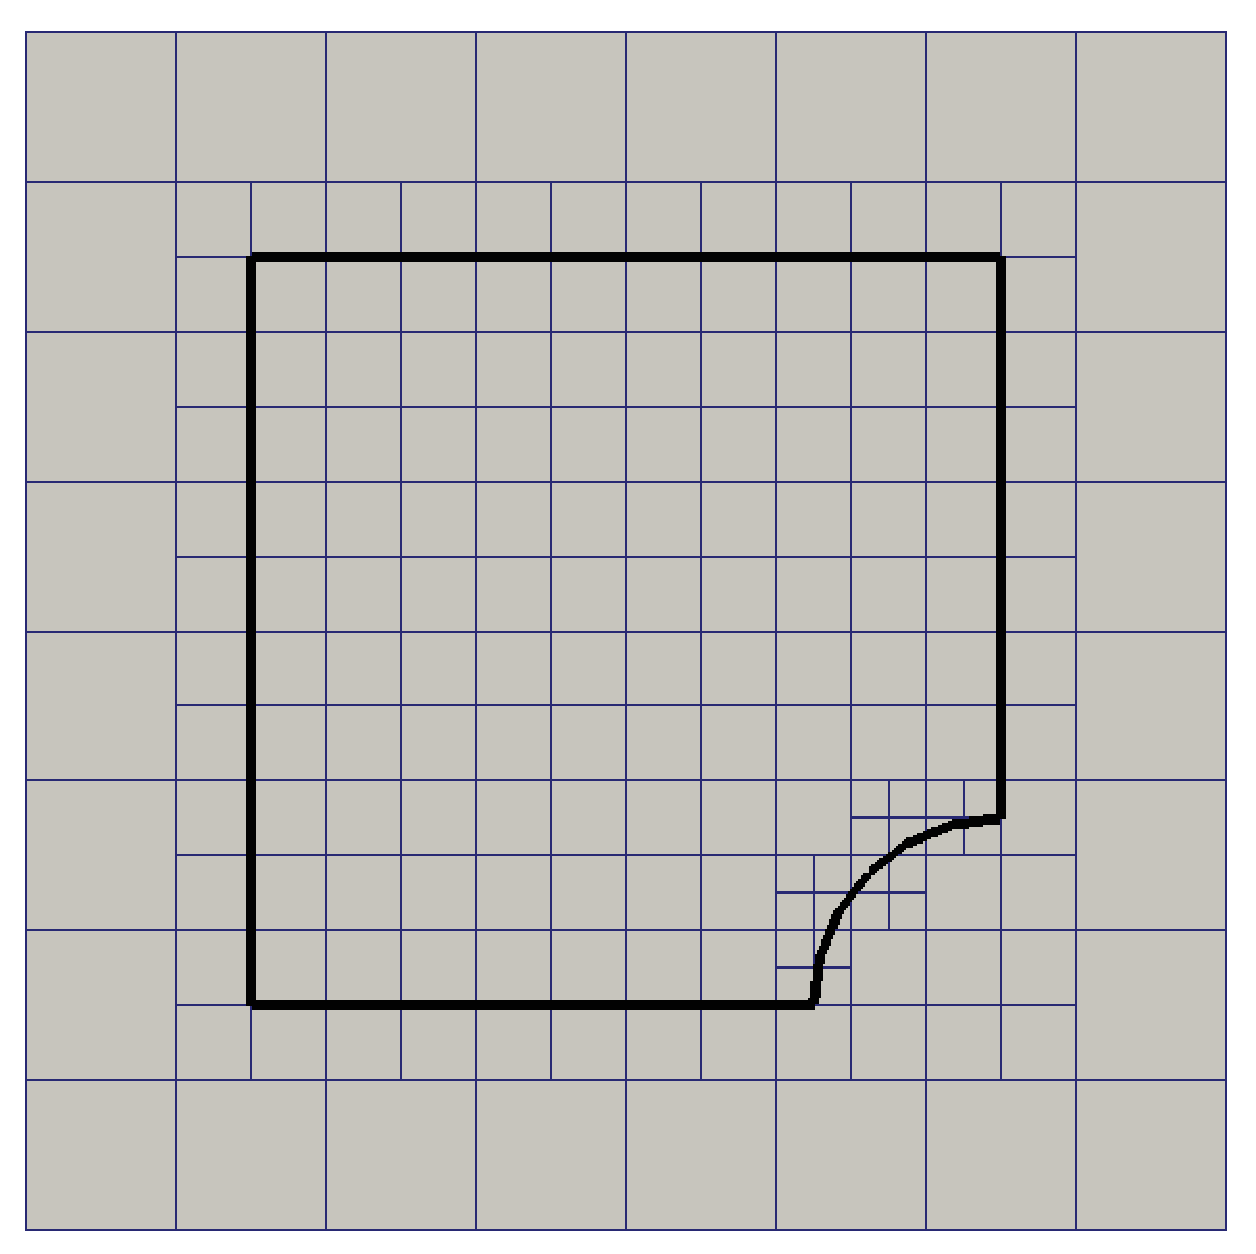
\includegraphics{quadtree/ex_images/ex_chole_background.eps}
    }
    \caption[Background mesh of infinite plate with a circular hole]{Background mesh of infinite plate with a circular hole : Bold lines represents the input geometry}
    \label{qdt_fig:ex_chole_background_mesh}
\end{figure}

\begin{figure}
    \centering
    \scalebox{0.35}{
        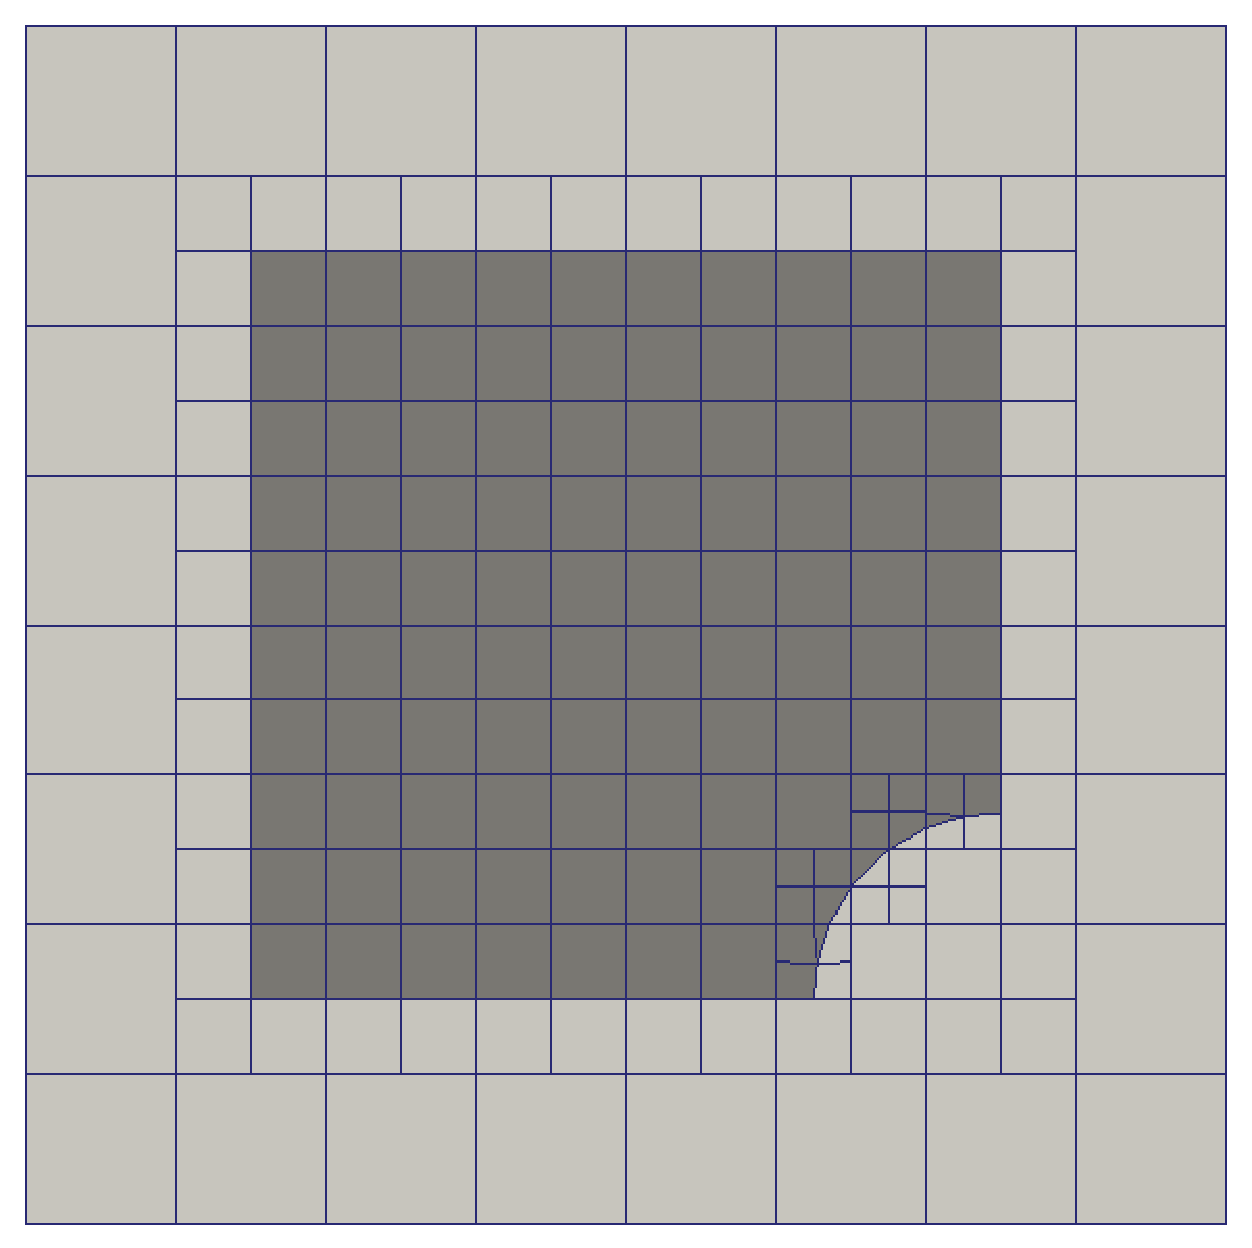
\includegraphics{quadtree/ex_images/ex_chole_coloring.eps}
    }
    \caption[Mesh coloring of infinite plate with a circular hole]{Mesh coloring of infinite plate with a circular hole : Grey area represents the plate}
    \label{qdt_fig:ex_chole_mesh_coloring}
\end{figure}

\begin{figure}
    \centering
    \scalebox{0.35}{
        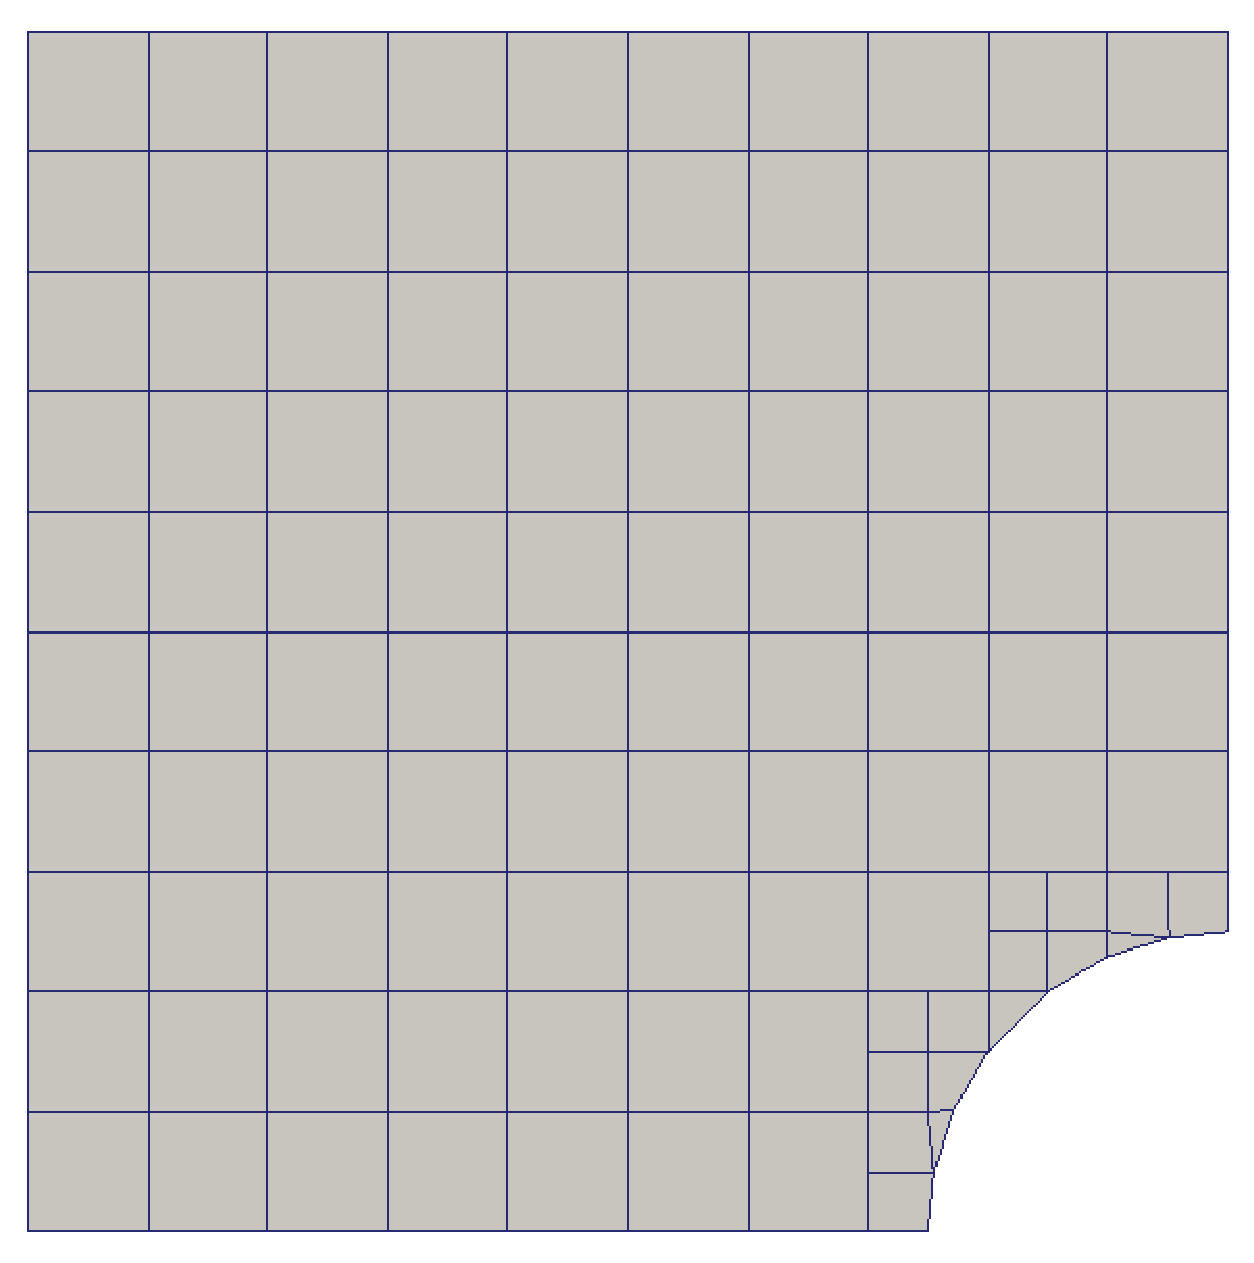
\includegraphics{quadtree/ex_images/ex_chole_mesh_262.eps}
    }
    \caption[Final mesh of infinite plate with a circular hole]{Final mesh of infinite plate with a circular hole}
    \label{qdt_fig:ex_chole_mesh_final}
\end{figure}
% 262 - 0.0112 (32-4/5-4)
% 290 - 0.0101 (64-4/5-4)
% 876 - 0.0036216 (128-4/8-4)
% 3280- 0.0010068 (256-4/15-4)
\paragraph{}
Mesh with different parameters are plotted in Fig.~\ref{qdt_fig:ex_chole_mesh_all} and the convergence study is plotted in Fig.~\ref{qdt_fig:ex_chole_mesh_conv}

\begin{figure}[H]
    \begin{subfigure}[b]{1\linewidth}
        \centering
        \scalebox{0.35}{
            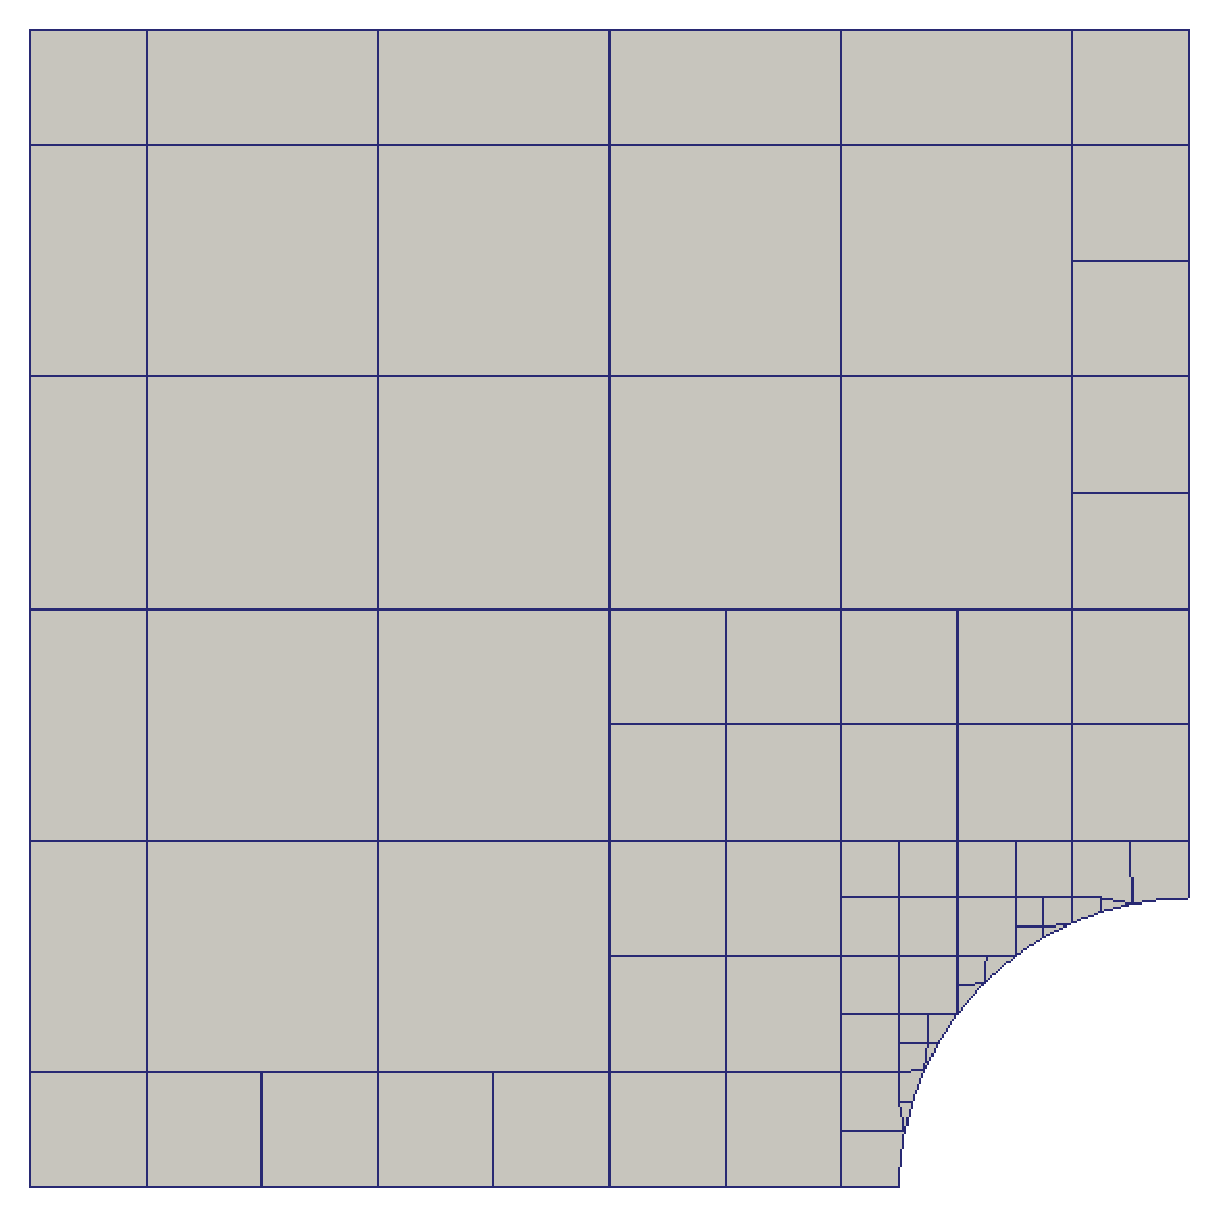
\includegraphics{quadtree/ex_images/qdt_chole_64_8.eps}
        }
        \caption{Mesh with $res=64$, $s_{max}=8$, 152 DOFs}
    \end{subfigure}
    \\
    \begin{subfigure}[b]{1\linewidth}
        \centering
        \scalebox{0.35}{
            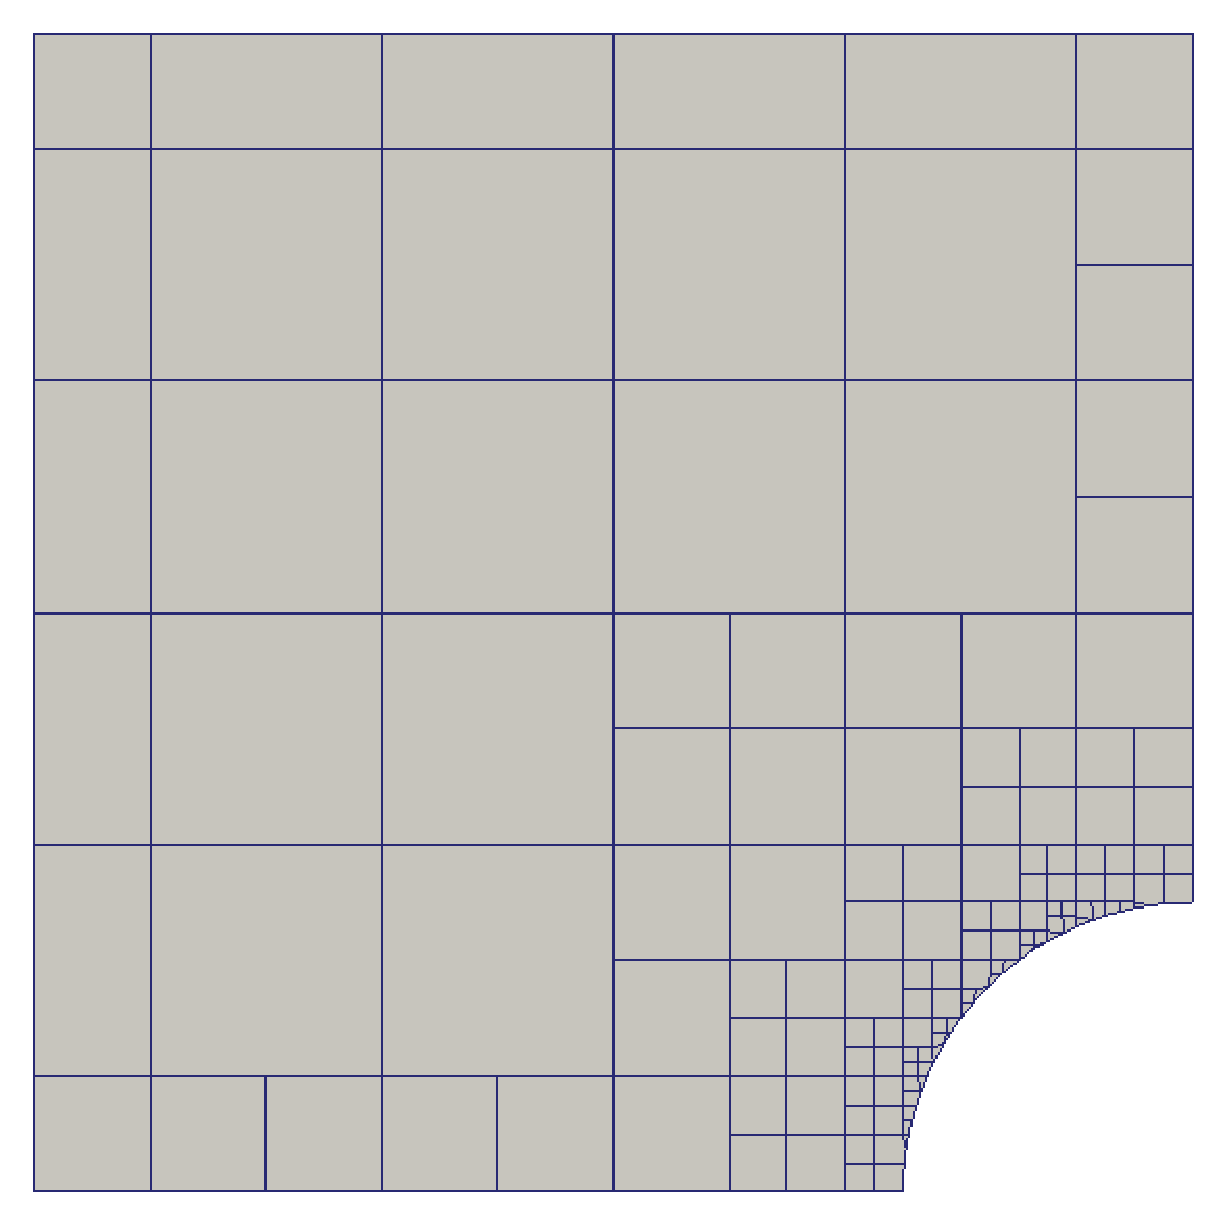
\includegraphics{quadtree/ex_images/qdt_chole_128_16.eps}
        }
        \caption{Mesh with $res=128$, $s_{max}=4$, 272 DOFs}
    \end{subfigure}
\end{figure}

\begin{figure}[H]\ContinuedFloat
    \begin{subfigure}[b]{1\linewidth}
        \centering
        \scalebox{0.35}{
            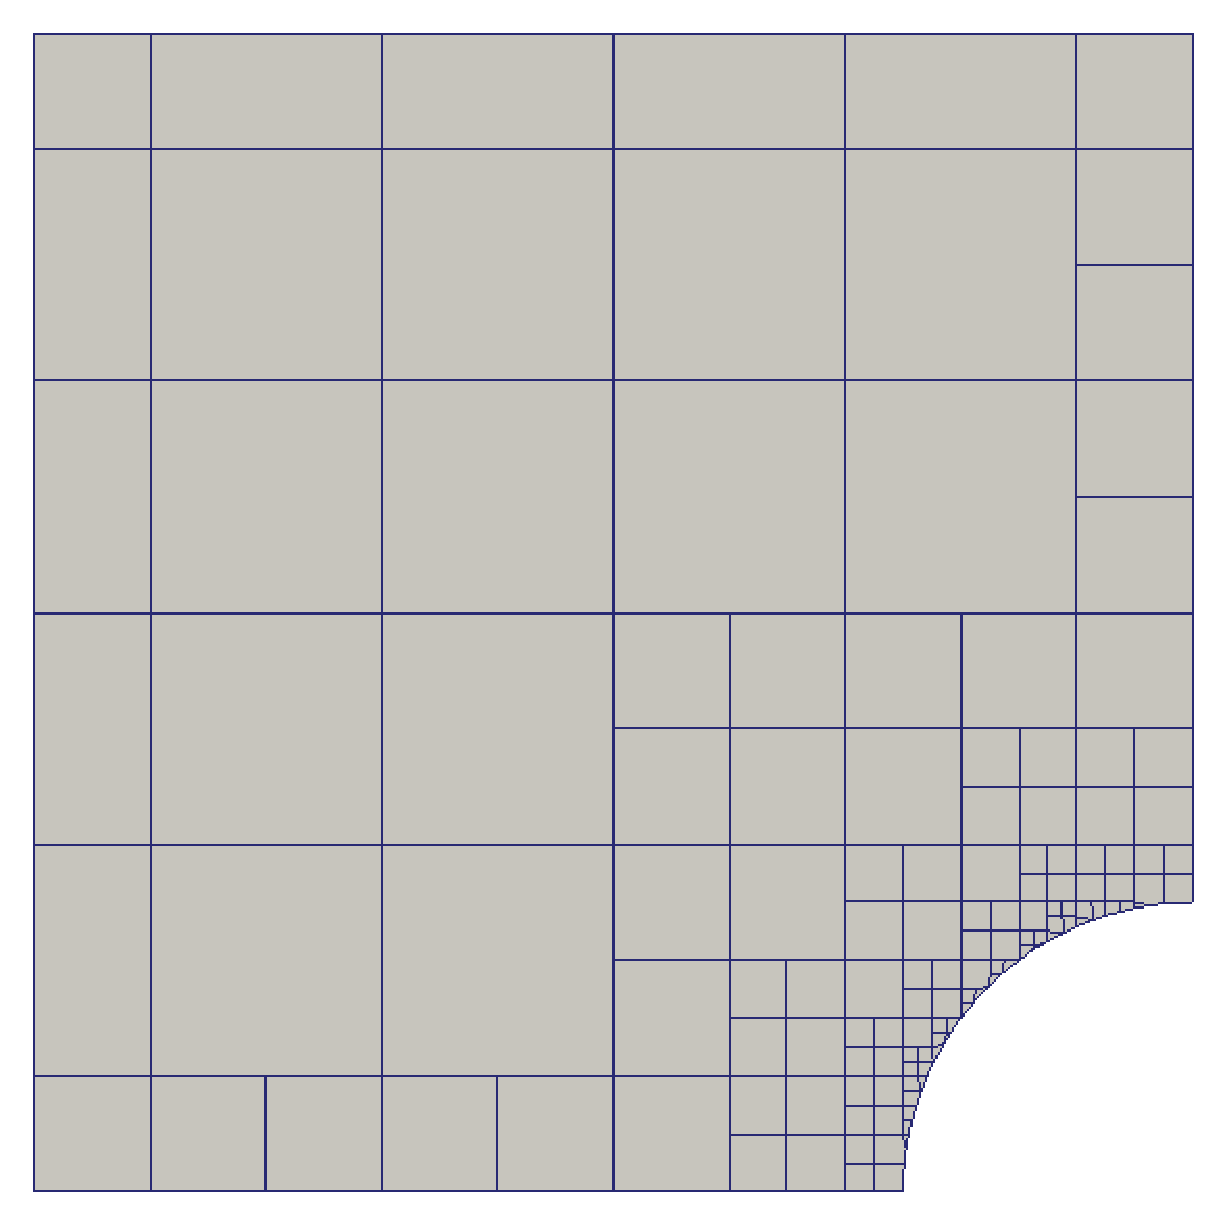
\includegraphics{quadtree/ex_images/qdt_chole_128_16.eps}
        }
        \caption{Mesh with $res=128$, $s_{max}=16$, 488 DOFs}
    \end{subfigure}
    \caption[Mesh of the infinite plate with a circular hole]{Mesh of infinite plate with a circular hole}
    \label{qdt_fig:ex_chole_mesh_all}
\end{figure}


\begin{figure}[H]
    \centering
    \scalebox{0.6}{
        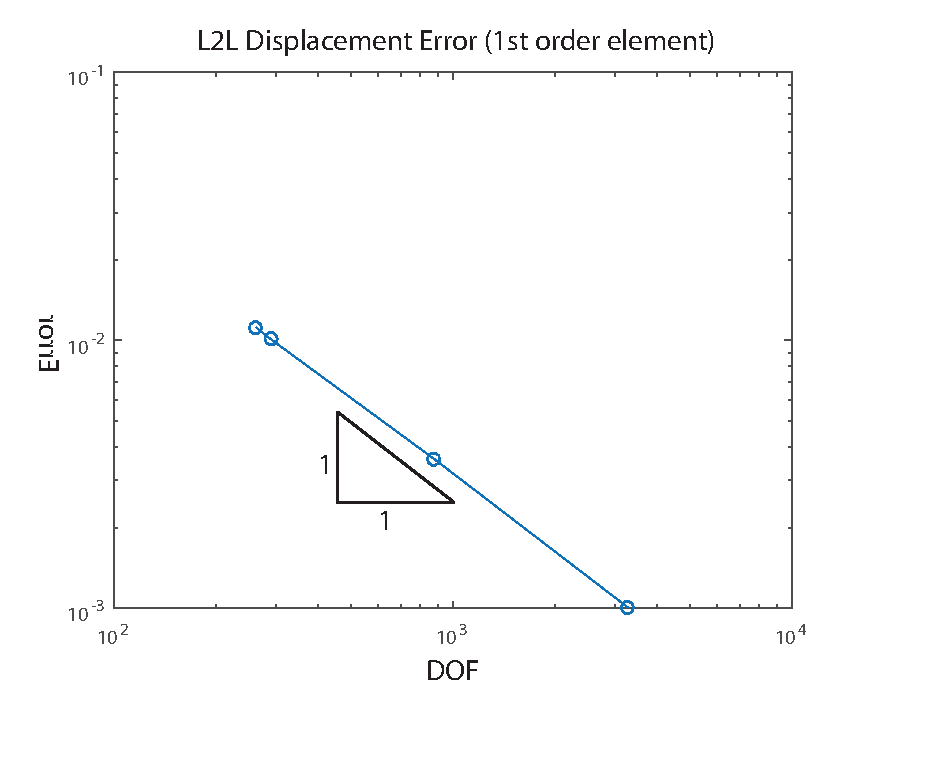
\includegraphics{quadtree/ex_images/ex_chole_conv.eps}
    }   
    \caption[Convergence of the infinite plate with a circular hole]{Convergence of the infinite plate with a circular hole}
    \label{qdt_fig:ex_chole_mesh_conv}
\end{figure}

\pagebreak
\subsection{Plane strain bracket}
\paragraph{}
In this example, a plane strain bracket with a downward uniform distributed load on the top is considered (see fig.~\ref{qdt_fig:ex_bracket_geo_bc}).
The material properties are: Young’s modulus $E = 2\times 10^5 N/m^2$ and Poisson’s ratio $\nu = 0.3$.
    \begin{figure}[H]
        \centering
        \begin{subfigure}[b]{1\linewidth}
            \centering
            \scalebox{1.5}{
                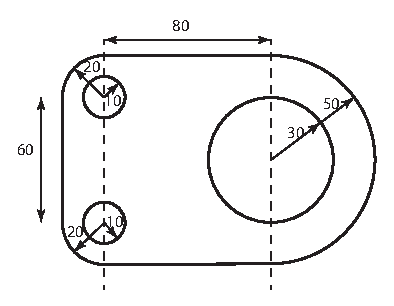
\includegraphics{quadtree/ex_images/ex_bracket_geo.eps}
            }
        \end{subfigure}
        \begin{subfigure}[b]{1\linewidth}
            \centering
            \scalebox{1.5}{
                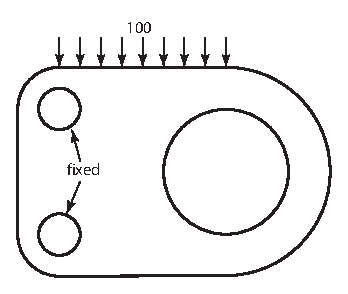
\includegraphics{quadtree/ex_images/ex_bracket_load.eps}
            }
        \end{subfigure}
        \caption{ Plane strain bracket: geometry and boundary conditions}
        \label{qdt_fig:ex_bracket_geo_bc}
    \end{figure}

\paragraph{}
A total strain energy of $282.927$ is determined by ANSYS with the mesh shown in fig.~\ref{qdt_fig:ex_bracket_ansys_mesh}
    \begin{figure}[H]
        \centering
        \scalebox{0.35}{
            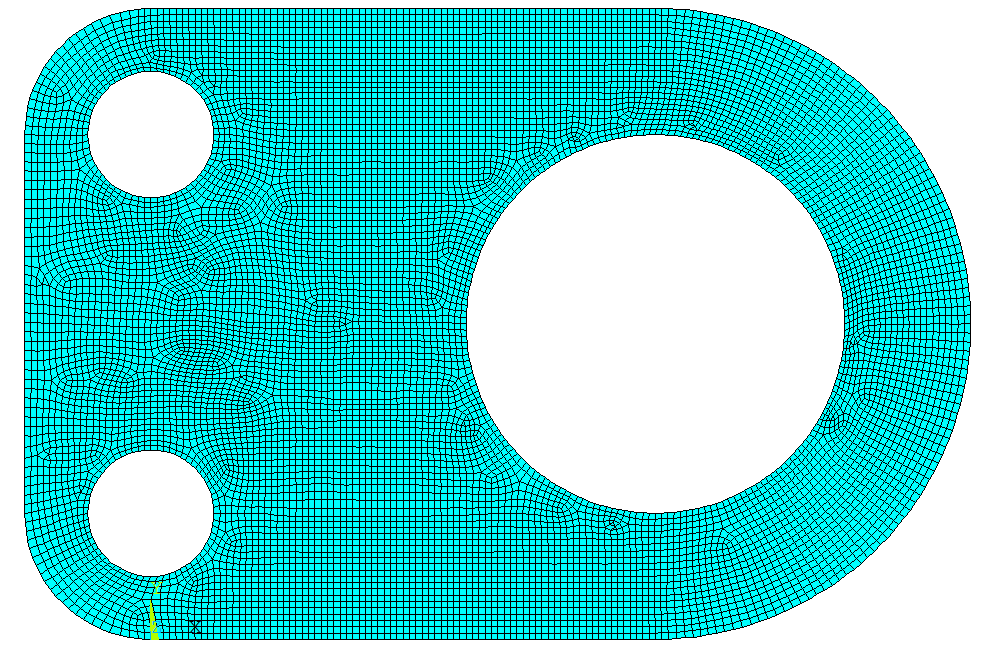
\includegraphics{quadtree/ex_images/ex_bracket_ansys_mesh_31002nodes.png}
        }
        \caption{ANSYS mesh for plane strain bracket (62004 DOF)}
        \label{qdt_fig:ex_bracket_ansys_mesh}
    \end{figure}

\paragraph{}
Drawing in AutoCAD will be divided into two parts: base and the holes as shown in fig.~\ref{qdt_fig:ex_bracket_cad}
    \begin{figure}[H]
        \centering
        \begin{subfigure}[b]{1\linewidth}
            \centering
            \scalebox{0.4}{
                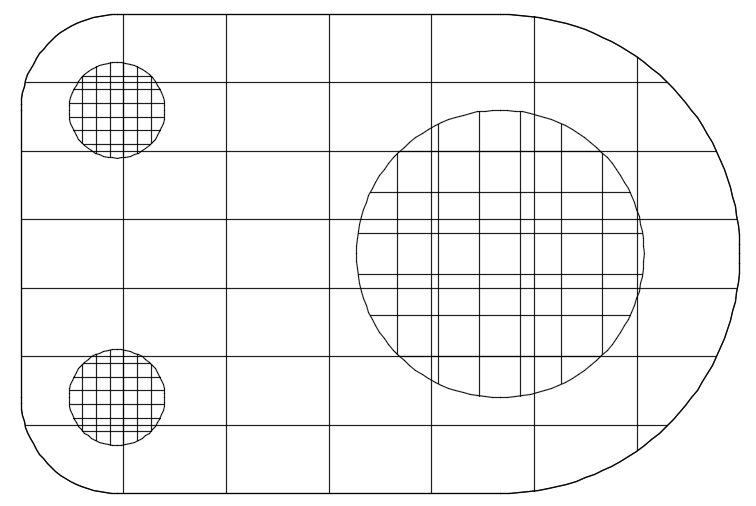
\includegraphics{quadtree/ex_images/ex_bracket_cad_full.png}
            }
            \caption{All}
        \end{subfigure}
        \begin{subfigure}[b]{0.4\linewidth}
            \scalebox{0.2}{
                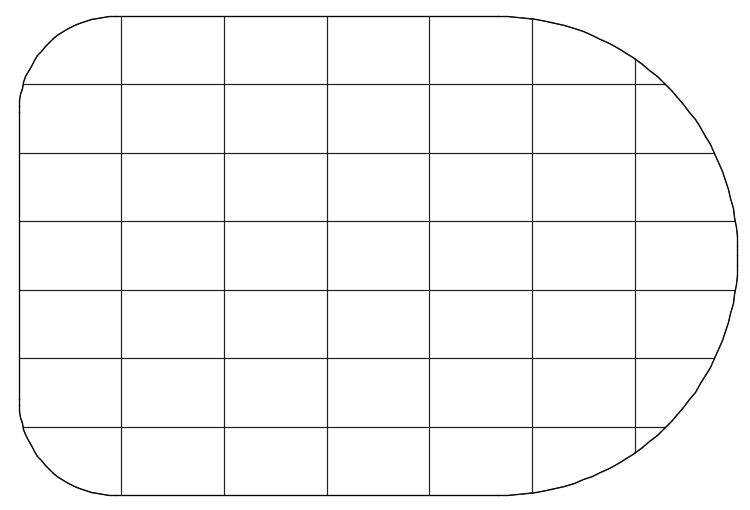
\includegraphics{quadtree/ex_images/ex_bracket_cad_base.png}
            }
            \caption{Base}
        \end{subfigure}
        \begin{subfigure}[b]{0.4\linewidth}
            \scalebox{0.2}{
                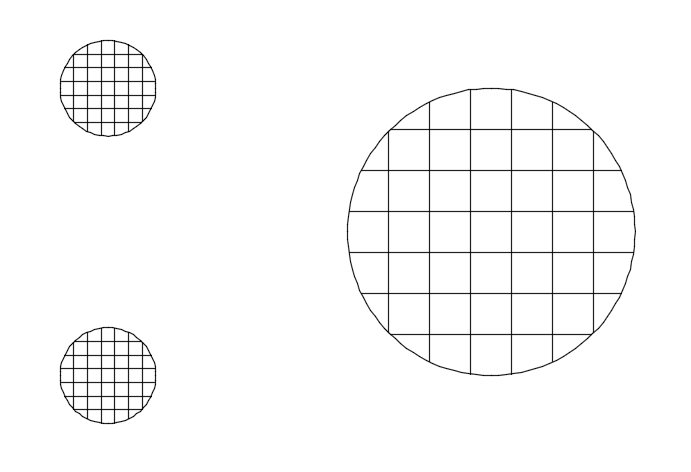
\includegraphics{quadtree/ex_images/ex_bracket_cad_holes.png}
            }
            \caption{Holes}
        \end{subfigure}
        \caption{CAD drawing of plane strain bracket}
        \label{qdt_fig:ex_bracket_cad}
    \end{figure}
% fig- 64,32/8,3
Generated background mesh, coloring and the final result with $res=32$, $s_{max}=4$ and $s_{min}=1$ are shown in fig.~\ref{qdt_fig:ex_chole_background_mesh}, fig.~\ref{qdt_fig:ex_chole_mesh_coloring} and fig.~\ref{qdt_fig:ex_chole_mesh_final}.
\begin{figure}
    \centering
    \scalebox{0.4}{
        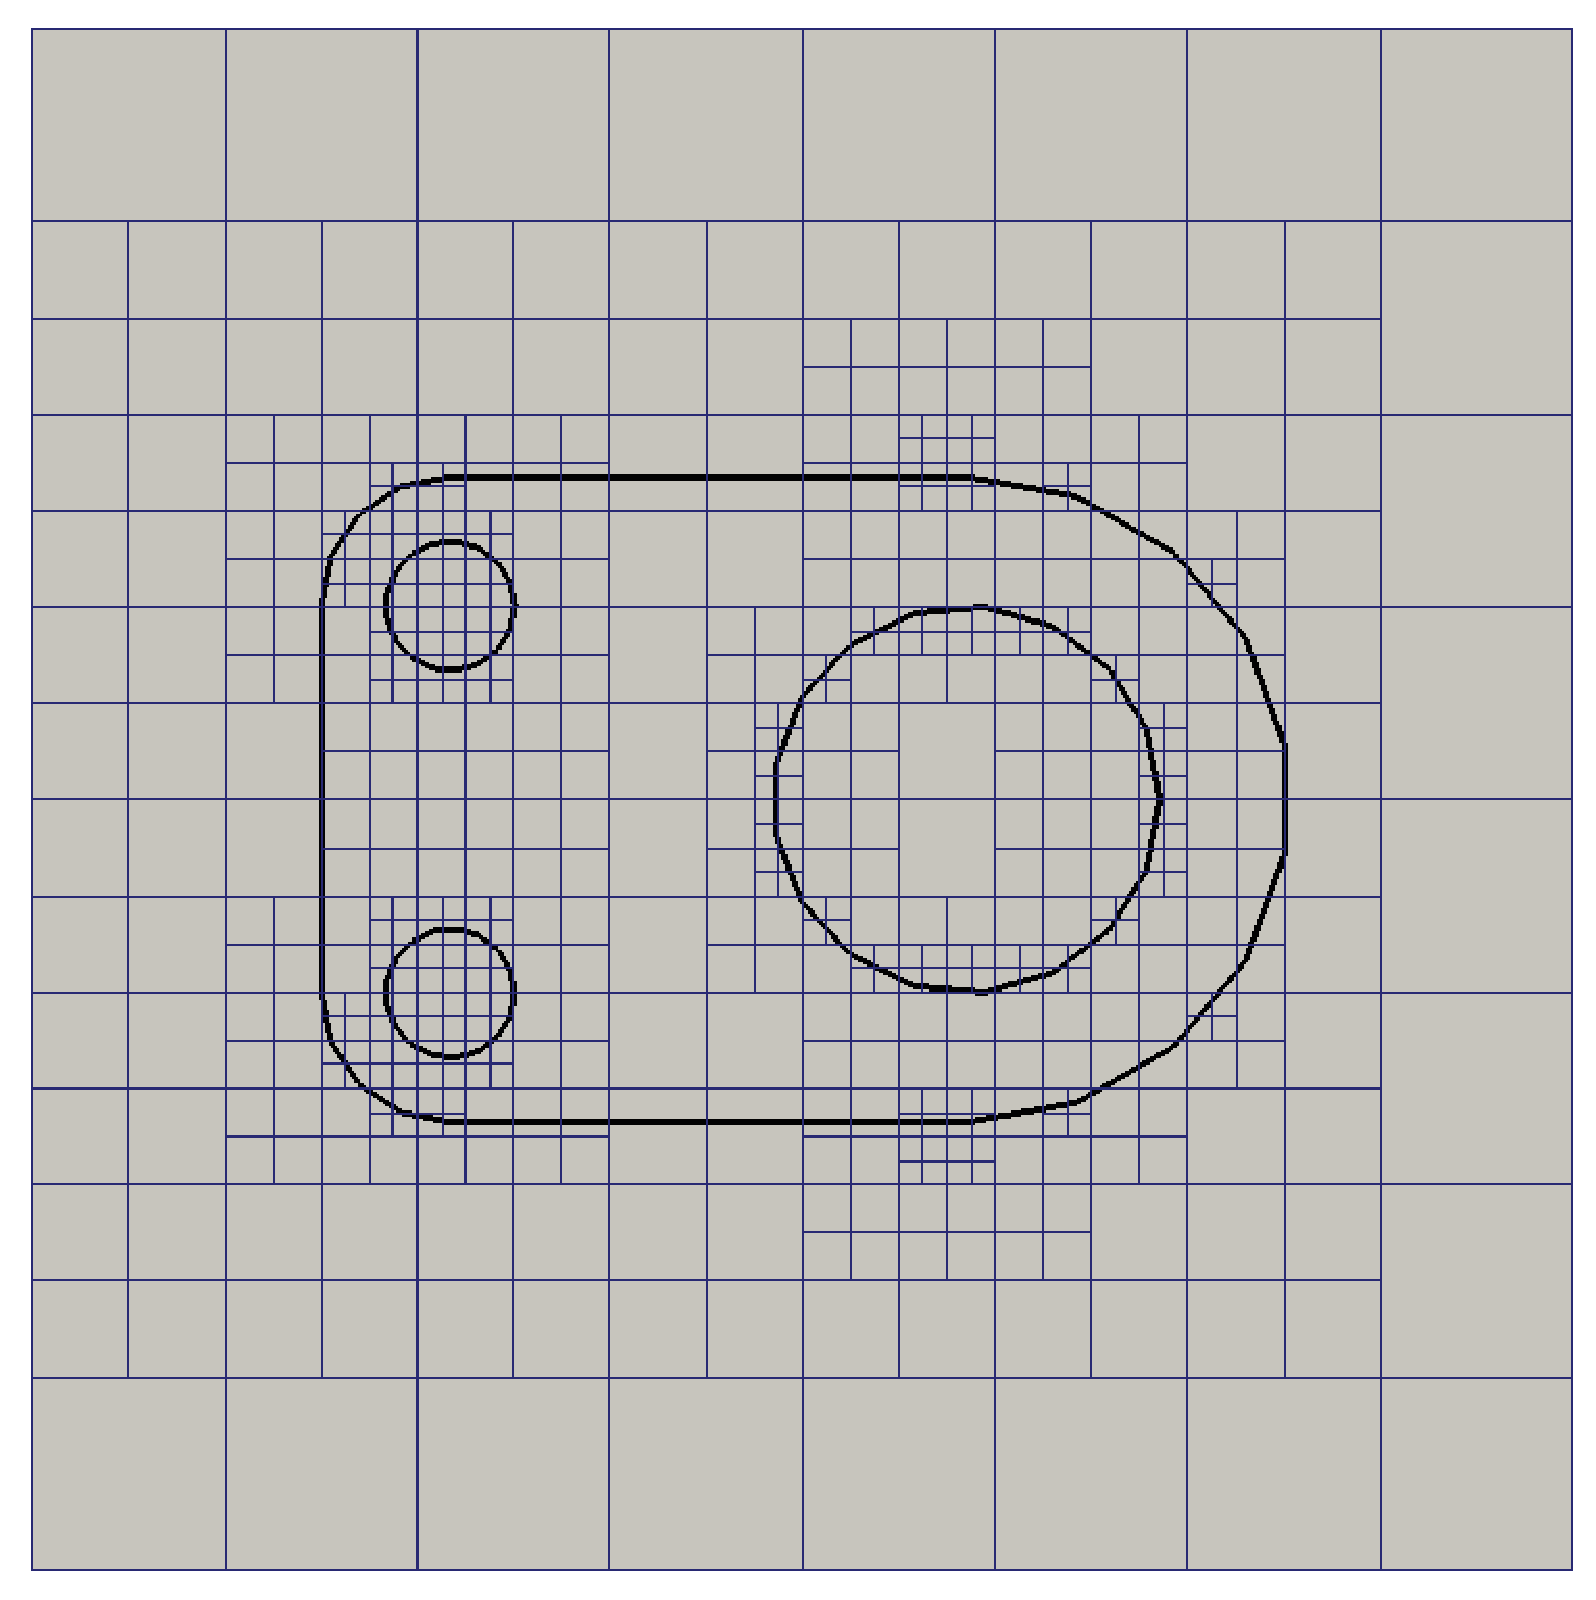
\includegraphics{quadtree/ex_images/ex_bracket_background.eps}
    }
    \caption[Background mesh of the bracket]{Background mesh of the bracket : Bold lines represents the input geometry}
    \label{qdt_fig:ex_chole_background_mesh}
\end{figure}

\begin{figure}
    \centering
    \scalebox{0.4}{
        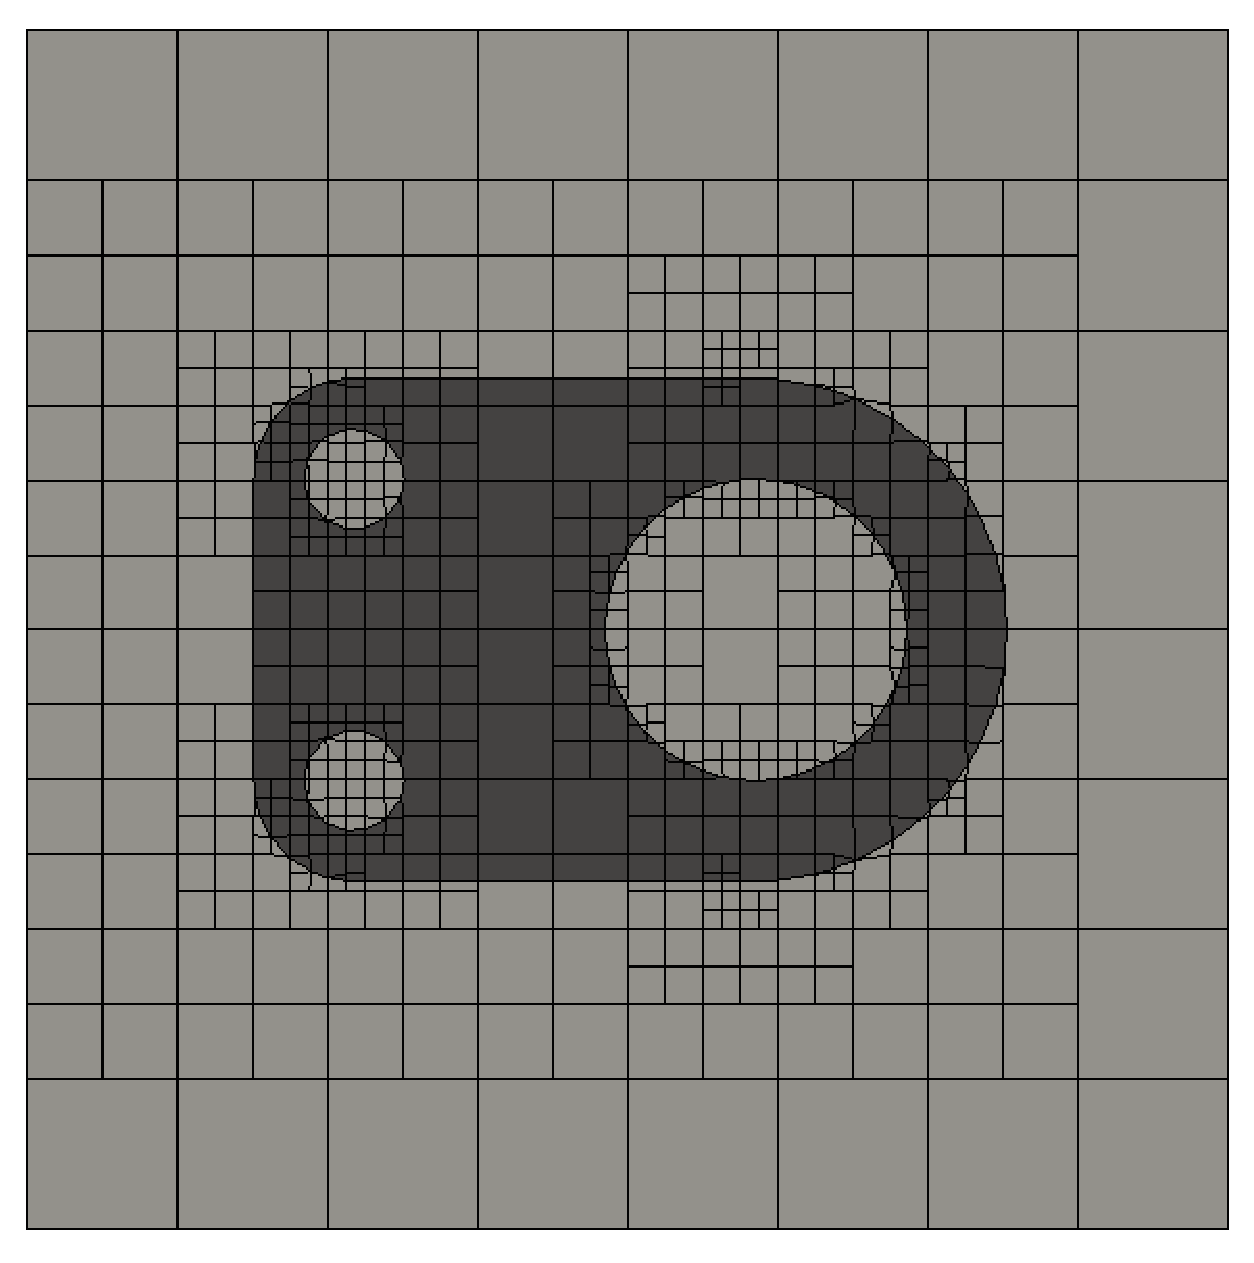
\includegraphics{quadtree/ex_images/ex_bracket_colored.eps}
    }
    \caption[Mesh coloring of the bracket]{Mesh coloring of the bracket : Grey area represents the bracket}
    \label{qdt_fig:ex_chole_mesh_coloring}
\end{figure}

\begin{figure}
    \centering
    \scalebox{0.3}{
        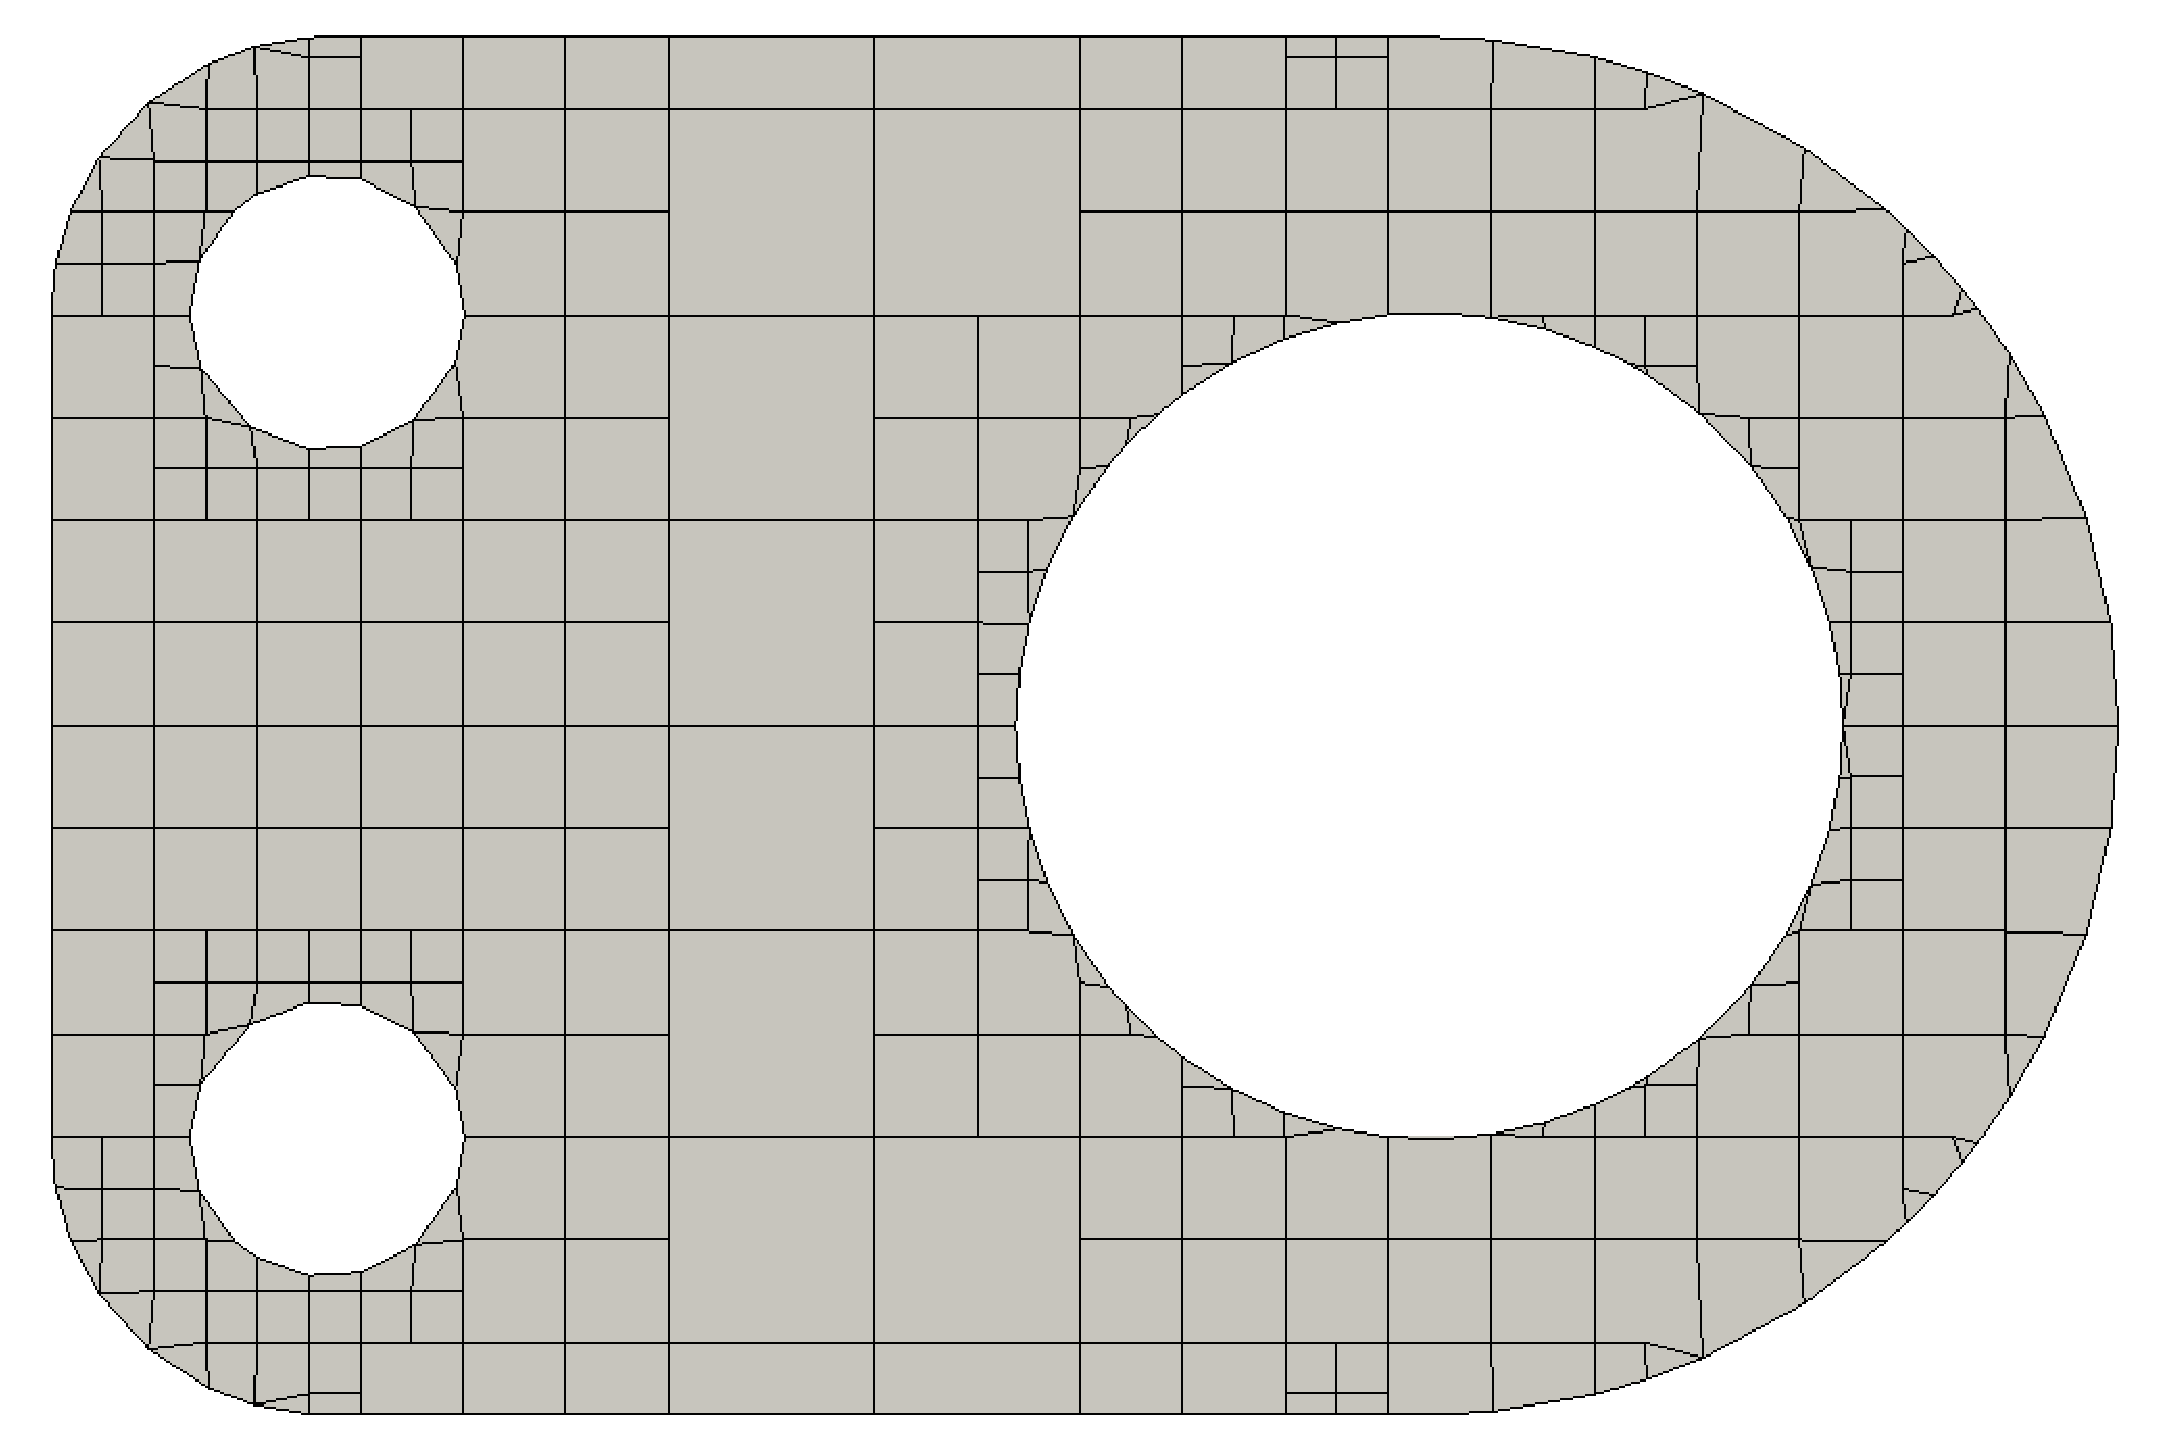
\includegraphics{quadtree/ex_images/ex_bracket_final.eps}
    }
    \caption[Final mesh of the bracket]{Final mesh of the bracket}
    \label{qdt_fig:ex_chole_mesh_final}
\end{figure}
% -1 - 282.927
% 382*2  - 274.5638 (32-4/8-3)
% 950*2  - 280.1255 (64-4/8-3)
% 2110*2 - 281.0799 (128-4/15-4)
% 4414*2 - 282.0363 (256-4/15-4)
Mesh with different parameters are plotted in fig.~\ref{qdt_fig:ex_bracket_mesh_all} and the convergence study is plotted in fig.~\ref{qdt_fig:ex_bracket_mesh_conv}

\begin{figure}[H]
    \begin{subfigure}[b]{1\linewidth}
        \centering
        \scalebox{0.4}{
            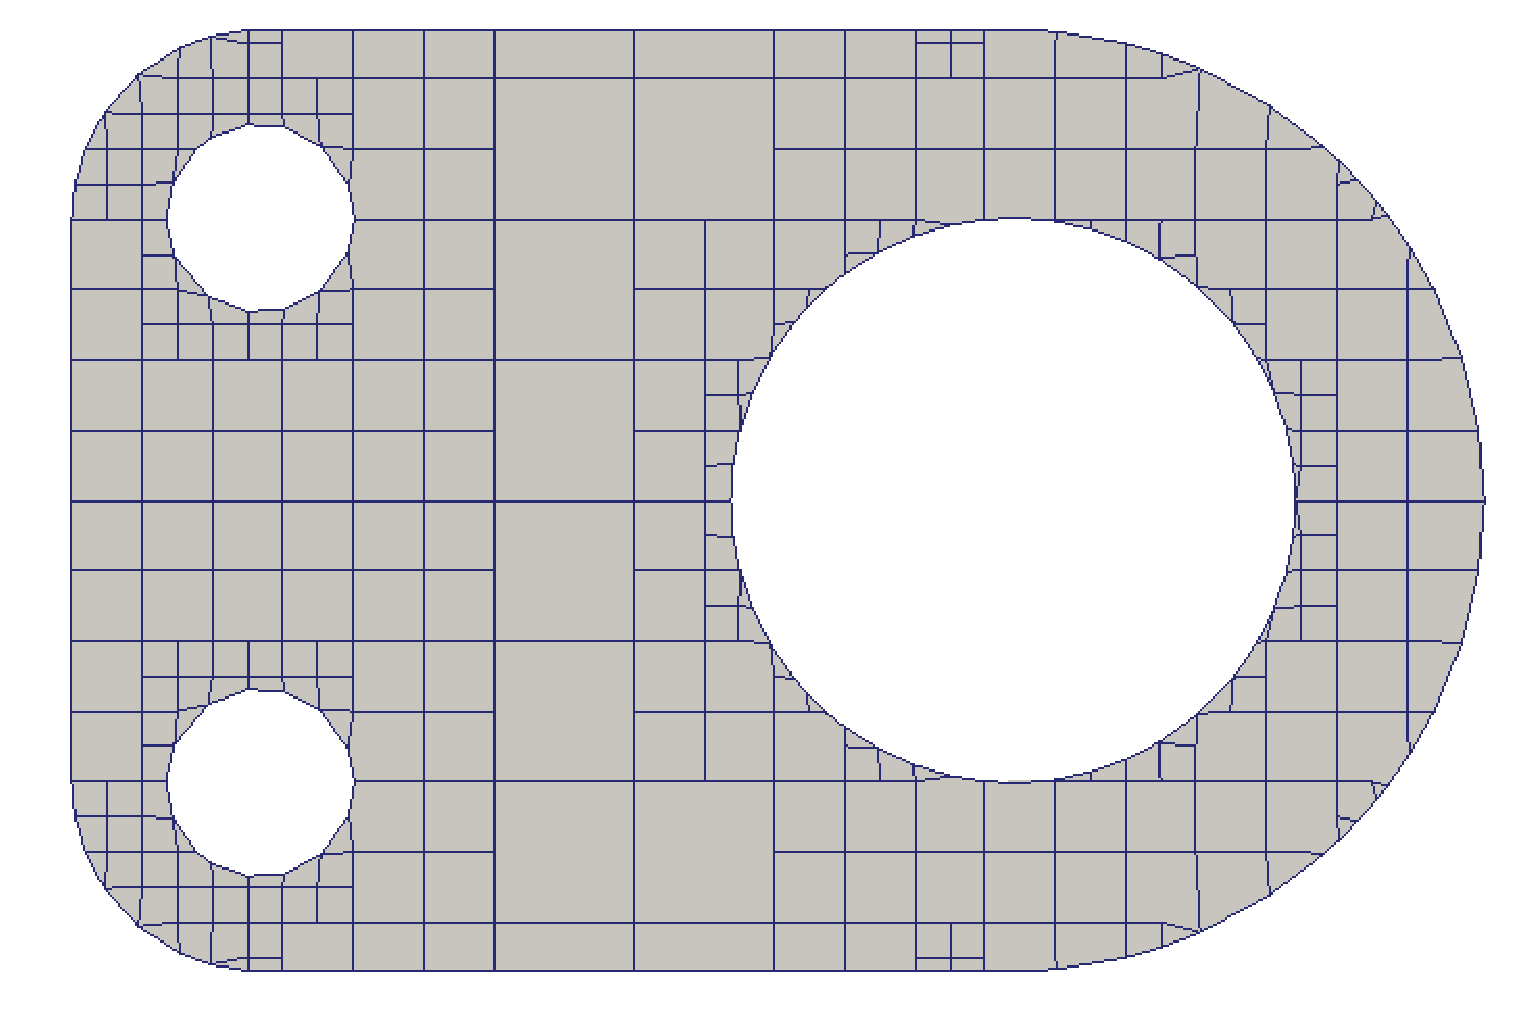
\includegraphics{quadtree/ex_images/ex_bracket_mesh_64_4.eps}
        }
        \caption{Mesh with $res=64$, $s_{max}=4$, 1656 DOFs}
    \end{subfigure}
    \\
    \begin{subfigure}[b]{1\linewidth}
        \centering
        \scalebox{0.4}{
            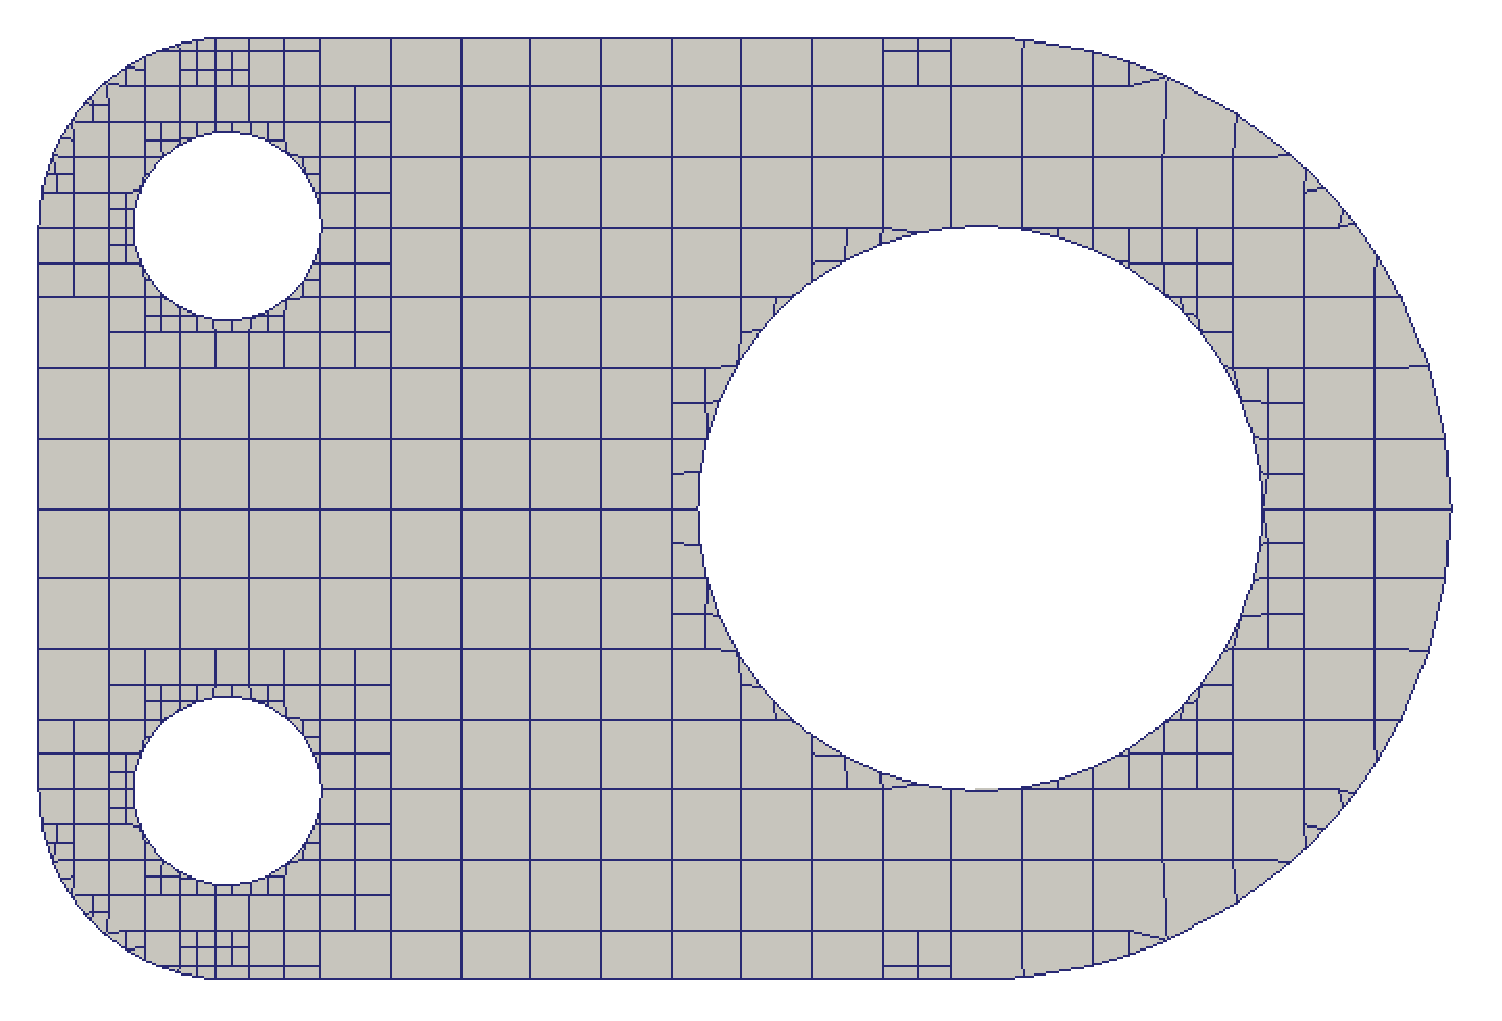
\includegraphics{quadtree/ex_images/ex_bracket_mesh_128_4.eps}
        }
        \caption{Mesh with $res=128$, $s_{max}=4$, 2548 DOFs}
    \end{subfigure}
\end{figure}

\begin{figure}[H]\ContinuedFloat
    \begin{subfigure}[b]{1\linewidth}
        \centering
        \scalebox{0.5}{
            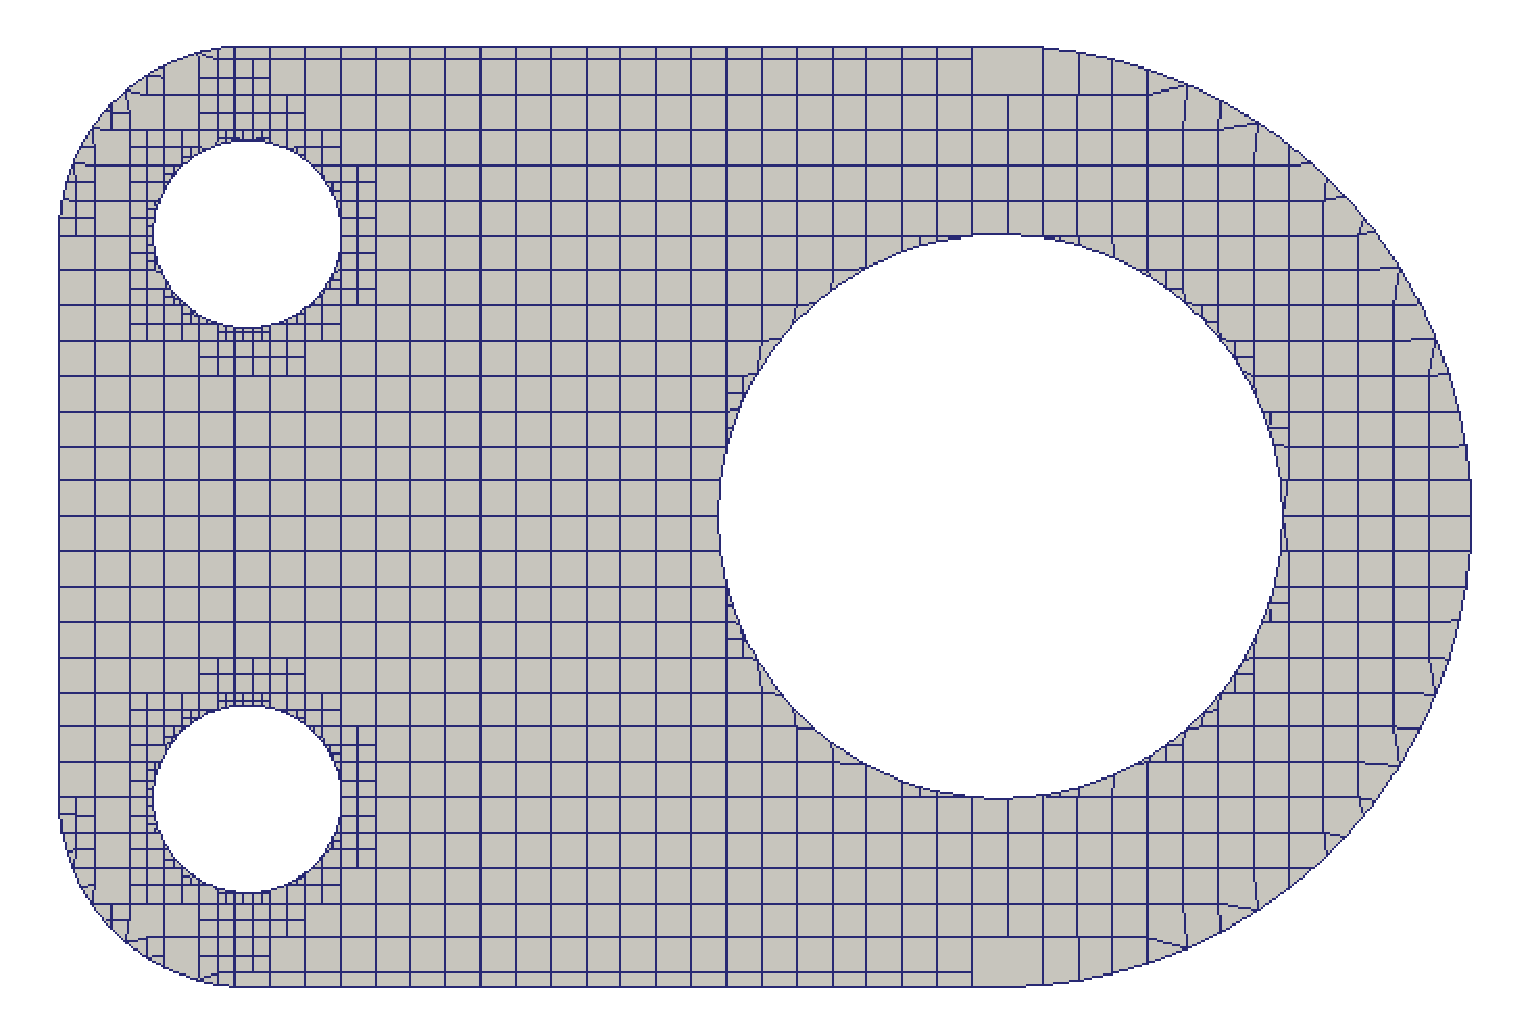
\includegraphics{quadtree/ex_images/ex_bracket_mesh_256_4.eps}
        }
        \caption{Mesh with $res=256$, $s_{max}=4$, 5464 DOFs}
    \end{subfigure}
    \caption[Mesh of the plane strain bracket]{Mesh of the plane strain bracket}
    \label{qdt_fig:ex_bracket_mesh_all}
\end{figure}

\begin{figure}[H]
    \centering
    \scalebox{0.75}{
        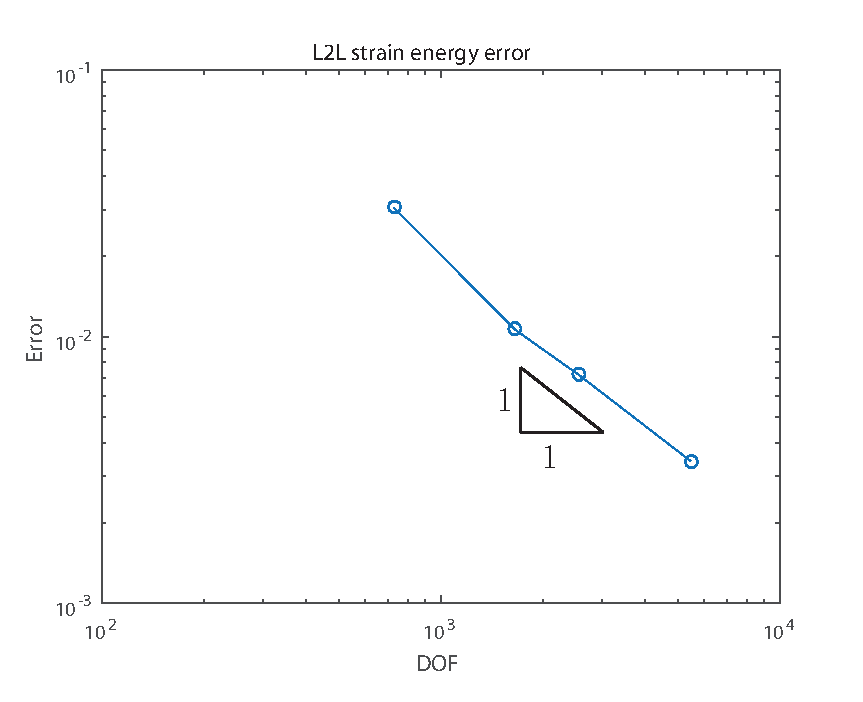
\includegraphics{quadtree/ex_images/ex_bracket_conv.eps}
    }   
    \caption[Convergence of the plane strain bracket]{Convergence of the plane strain bracket}
    \label{qdt_fig:ex_bracket_mesh_conv}
\end{figure}


\paragraph{}
Fig.~\ref{qdt_fig:bracket_stress_contour} shows the von Mises equivalent stress for the plane strain bracket.
From Fig.~\ref{qdt_fig:bracket_stress_contour}, it can be observed that the results from the present approach qualitatively match with the FE solution.
\begin{figure}[h!]
    \begin{subfigure}[b]{1\linewidth}
        \centering
        \scalebox{0.4}{
            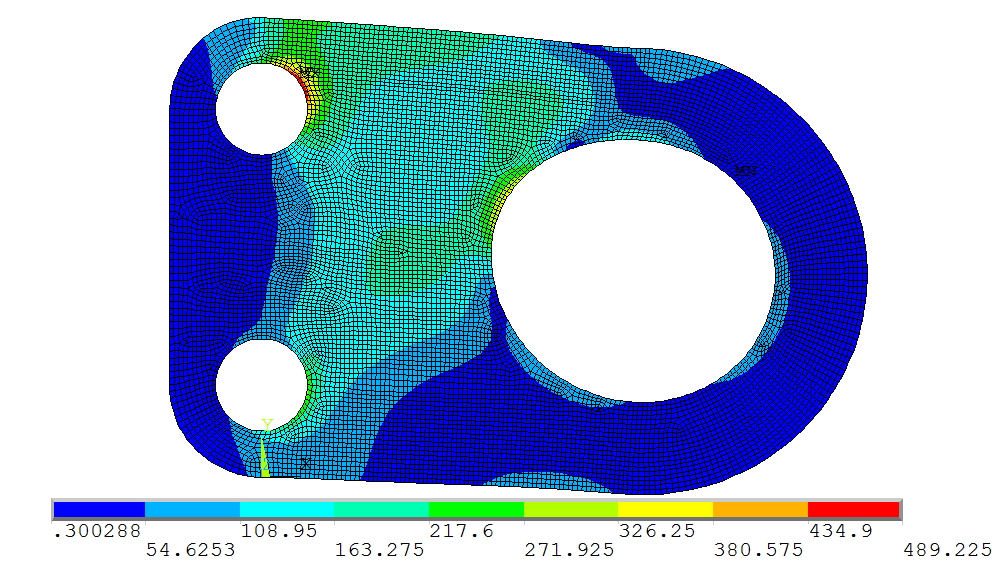
\includegraphics{quadtree/ex_images/ex_bracket_ansys_vmstr.png}
        }
        \caption{FEM}
    \end{subfigure}
    \begin{subfigure}[b]{1\linewidth}
        \centering
        \scalebox{0.4}{
            \includegraphics{quadtree/ex_images/ex_bracket_strcontour.eps}
        }
        \caption{Quadtree SBFEM}
    \end{subfigure}

    \caption{Von Mises equivalent stress contours for plane strain bracket}
    \label{qdt_fig:bracket_stress_contour}
\end{figure}
\input{quadtree/ex_dam.tex}
\subsection{Buildings on the ground}

\begin{figure}
    \centering
    \scalebox{0.5}{
        \includegraphics{quadtree/ex_images/ex_building_stress.eps}
    }
    \caption{Von-mises stress contour for the buidlings on the ground}
    % \label{qdt_fig:ex_cantilever_beam_background_mesh}
\end{figure}

\section{Conclusions}              % chapter 4
% %!TEX root = ../thesis.tex

\chapter{Adaptivity}

\section{Introduction}

\section{Lambda error indicator in SBFEM}
\subsection{Principal component analysis(PCA)}

\section{Mesh optimization}

\subsection{Merge triangle}
\subsection{Points moving}

\pagebreak
\section{Matrix reprensentation of NURBS}
\label{adap_sec_mrep2d}
\subsection{Implicit Matrix Representation}
\label{adap_sec:mrep}
\paragraph{} 
Matrix representation of a parameterized algebraic curve allows an easy way to calculate the intersection between it with another curve and find the corresponding parameter based on the given point on the curve.
For an algebraic curve $t \in \mathbf{R}^1 \xrightarrow{\phi} \left( \frac{f_1(t)}{f_0(t)}, \frac{f_2(t)}{f_0(t)},\frac{f_3(t)}{f_0(t)} \right) \in \mathbf{R}^3$, $f_0,f_1,f_2$ and $f_3$ are polynomials functions in parameter $t$ with degree $\leq p$.
The procedure of constructing the matrix representation for NURBS curves are explained detail in \citep{Laurent2014}.
\paragraph{}
The aim of this method is to find 4-tuples of polynomials\\
$\left( g_0(t),g_1(t),g_2(t),g_3(t) \right)$ with order $v$ so that
\begin{equation}
    \sum_{i=0}^3 g_i(t) f_i(t) \equiv 0
    \label{adap_eq_mRep_eq0}
\end{equation}
%
who is a vector space and one of its bases can be:
\begin{equation}
    \mathbf{L_j}(t,X,Y,Z) = g_0(t) + Xg_1(t) + Yg_2(t) + Zg_3(t)
    \label{adap:eq:mrep_eq1}
\end{equation}
Since $g$ is also a polynomial based function, it can be expressed in the vector space with a set of bases of $\left\{\psi_1(t), \psi_2(t), \dots, \psi_{m_v}(t) \right\}$ and the bases $\mathbf{L_j}$ can be expressed as
    \begin{equation}
        \begin{aligned}
            \mathbf{L_j} &= \sum^{m_v}_{i=1}\left( \lambda_{0,i}^{(j)} + \lambda_{1,i}^{(j)}X + \lambda_{2,i}^{(j)}Y + \lambda_{3,i}^{(j)}Z\right)\psi_i(t)\\
        & = \sum_{i=1}^{m_v} \Lambda_{i,j}(X,Y,Z)\psi_i(t)
        \end{aligned}
    \end{equation}
%
Finally, a matrix which represents the mapping of $\phi$ in a $m_v \times r_v$-matrix $\mathbf{M_v}$ with order $v$
    \begin{equation}
        \mathbf{M_v}(\phi) = 
        \begin{bmatrix}
        \Lambda_{1,1} & \Lambda_{1,2} & \dots & \Lambda_{1,r_v} \\ 
        \Lambda_{2,1} & \Lambda_{2,2} & \dots & \Lambda_{2,r_v} \\ 
        \vdots 		  & \vdots 		  &  	  &\vdots			\\
        \Lambda_{m_v,1}&\Lambda_{m_v,2}&\dots &\Lambda_{m_v,r_v}
        \end{bmatrix}
    \end{equation}



%=====================================================================================================================%
\subsection{Matrix Representation for Rational Bézier Curves}
An rational bézier curves can be defined by 
\begin{equation}
	\phi:t\in \mathbf{R}\rightarrow \frac{\sum_{i=0}^pw_i\mathbf{P}_iB_i^p(t) }{\sum_{i=0}^pw_iB_i^p(t)}
\end{equation}
where
\begin{equation}
    B_i^p(t) = \mathbf{C}_i^dt^i(1-t)^{d-i}
    \label{adap_eq_mrep_bbasis}
\end{equation}
%
The aim is to find a matrix whose vector is in the form of
\begin{equation}
    [\alpha] =
    \begin{bmatrix}
        \alpha_{0,0} & \alpha_{0,1}&  \dots&  \alpha_{0,v} & \alpha_{1,0} & \dots & \alpha_{3,v} 
    \end{bmatrix}^T
\end{equation}
%
where $g_j(t)$ in Eq.~\ref{adap:eq:mrep_eq1} can be expressed as
\begin{equation}
    g_j(t) = \sum_{i=0}^v \alpha_{j,i}B_i^v(t)
\end{equation}
%
Based on Eq.~\eqref{adap_eq_mRep_eq0}, it can be concluded that $\mathbf{R}\times\left[\alpha\right]=0$
\begin{equation}
    \mathbf{R} = 
    \begin{bmatrix}
        B_0^v(t)f_0(t) & \dots & B_v^v(t)f_0(t) & B_0^v(t)f_1(t) & \dots & B_v^v(t)f_3(t)
    \end{bmatrix}
\end{equation}
%
By having another set of basis $\mathbf{L_v}$ and the transformation matrix $\mathbf{S}$ so that $\mathbf{L_vS}=\mathbf{R}$ where
\begin{equation}
    \mathbf{L_v}=
    \begin{bmatrix}
        B_0^{v+d}(t) & B_1^{v+d}(t) & \dots & B_{v+d}^{v+d}(t)
    \end{bmatrix}
\end{equation}
%
This leads to
\begin{equation}
    \begin{bmatrix}
        B_0^{v+d}(t) & B_1^{v+d}(t) & \dots & B_{v+d}^{v+d}(t)
    \end{bmatrix}\times \mathbf{S}\times\left[\alpha\right] = R\times\left[\alpha\right] = 0
\end{equation}
which indicates $\left[ \alpha\right]$ is in the null space of $\mathbf{S}$

After substituting $f(t) = \sum_{i=0}^dc_iB_i^d(t)$ into $\mathbf{R}$, the following can be deduced
\begin{equation}
    B_j^v(t)f(t) =  \sum_{i=0}^dc_iB_i^d(t)B_j^v(t) =\sum_{i=0}^d \frac{\mathbf{C}^v_j\mathbf{C}^d_i}{\mathbf{C}^{d+v}_{i+j}}c_i B_{i+j}^{d+v}(t)
\end{equation}
%
which indicates that
\begin{equation}
    \mathbf{S}_{i+j,j} = \frac{\mathbf{C}^v_j\mathbf{C}^d_i}{\mathbf{C}^{d+v}_{i+j}}c_i
\end{equation}
%
Finally, the null space of $\mathbf{S_v}$, $\mathbf{M_v}$ is the matrix representation of the rational bézier curve.



%=====================================================================================================================%
\subsection{Intersection}
The calculation of the intersection is described in detail in \citep{Buse2010, Ba2009}.
All intersections can be calculated at once by using matrix representation of the algebraic curve.
\paragraph{} 
Given a rational curve/surface $C1$
\begin{equation}
    \mathbf{P}^1 \xrightarrow{\phi_1} \mathbf{P}^n: (u,v) \rightarrow(f_0,f_1,f_2,f_3)(u,v)
\end{equation}
%
the aim is to find the intersection between it with another rational curve $C2$ via matrix representation
\begin{equation}
    \mathbf{P}^1 \xrightarrow{\phi_2} \mathbf{P}^n: (t) \rightarrow(g_0,g_1,g_2,g_3)(t)
\end{equation}
%
is to find
\begin{equation}
    \mathbf{M}_{v1}(\phi_2(t) = 0
\end{equation}
%
which leads to
\begin{equation}
    \mathbf{M_0}g_0 + \mathbf{M_1}g_1 + \mathbf{M_2}g_2 + \mathbf{M_3}g_3 = 0
    \label{mRep_intec_base}
\end{equation}
%
By knowing $g_n$ is a polynomial function with order $p$, Eq.~\eqref{mRep_intec_base} can be rearranged as
\begin{equation}
    \mathbf{M}(t) = \sum_{i=0}^p \mathbf{M_i}t^i
\end{equation}
%
After that, the generalized companion $q \times p$-matrices $A, B$ with rank $\rho$ are introduced
\begin{equation}
    A = 
    \begin{bmatrix}
        0		&I 		&\dots 		&\dots 		&0 		\\
        0 		&0 		&I 			&\dots 		&0 		\\
        \vdots 	&\vdots &\vdots 	&\vdots 	&\vdots \\
        0 		&0 		&\dots		&\dots 		&I 		\\
        M_0^t 	&M_1^t 	&\dots 		&\dots 		&M_{d-1}^t
    \end{bmatrix}
\end{equation}
%
\begin{equation}
    B = 
    \begin{bmatrix}
        I 		&0 		&\dots 		&\dots 		&0 		\\
        0 		&I 		&0 			&\dots 		&0 		\\
        \vdots 	&\vdots &\vdots 	&\vdots 	&\vdots \\
        0 		&0 		&\dots 		&I 			&0 		\\
        0 		&0 		&\dots 		&\dots 		&-M_d^t \\		
    \end{bmatrix}
\end{equation}
%
Before the eigenvalues are calculated, the regular part of a non-square pencil of the matrices shall be extracted first which is done by the following step
%
\paragraph{Step 1}
Transform $B$ into its column echelon form:
SVD-decomposition is adopted to perform the task.
\begin{equation}
\begin{aligned}
    B_1 = BV_0 = [\underbrace{B_{1,1}}_{\rho} |\underbrace{0}_{q-\rho}]	\\
    A_1 = AV_0 = [\underbrace{A_{1,1}}_{\rho} |\underbrace{A_{1,2}}_{q-\rho}]
\end{aligned}
\end{equation}
%
\paragraph{Step 2}
Transform $A_{1,2}$ into its row echelon form:
\begin{equation}
    U_1A_{1,2} = 
    \begin{bmatrix}
        \underline{A^\prime_{1,2}}\\
        0
    \end{bmatrix}
\end{equation}
%
where $A^\prime_{1,2}$ is in full row rank.\\
At the end of step 2, matrix $A$ and $B$ can be represented as
\begin{equation}
\begin{aligned}
    A^\prime_1 &=
    \begin{bmatrix}
        A^\prime_{1,1} & A^\prime_{1,2} \\
        \cmidrule(lr){1-2}
        A_2 & 0
    \end{bmatrix}\\
    B^\prime_1 &=
    \begin{bmatrix}
        B^\prime_{1,1} & 0\\
        \cmidrule(lr){1-2}
        B_2 & 0
    \end{bmatrix}
\end{aligned}
\end{equation}
where $A^\prime_{1,2}$ has full row rank\\
$
\begin{bmatrix}
\underline{B^\prime_{1,1}}\\
B_2
\end{bmatrix}
$ has full column rank\\
$
\begin{bmatrix}
\underline{B^\prime_{1,1}}\\
B_2
\end{bmatrix}
$ 
and $B_2$ are in echelon form
\paragraph{}
$A_2$ and $B_2$ will be the new $A$ and $B$ matrices for next iteration until $B$ has full rank.
If $B$ has full row rank but not full rank, $A=A^T$ and $B=B^T$ are conducted.
\paragraph{}
After these processes, $A$ and $B$ become two square matrices and $B$ is invertible so that the solution for the intersection parameter $t$ can be determined from the eigenvalue of the matrix $AB^{-1}$
\paragraph{}
However, the method may fail when the intersection is under the case where nearly tangential geometric conditions happens and return two empty matrices.
It is addressed by adding another step after extracting the real part of the $A$ and $B$ if the results are empty matrices\citep{Shen2016}.
If the input matrix $A$ and $B$ are not in full row rank or full column rank, it is considered that $C1 \cap C2 = C2$.
If the input matrix $A$ and $B$ are in full row rank or full column rank, a rank $m$ square sub-pencil is extracted assuming $A$ and $B$ have a rank of $m$.
Then the eigenvalues yield the intersections.


\section{Numerical examples}

\section{Conclusions}

            % chapter 5
% %!TEX root = ../thesis.tex

\chapter{Isogeometric enhanced SBFEM in 3D}
\section{Introduction}
\paragraph{}
This chapter starts with a mesh generated by the help of the octree based algorithm using STL file directly \citep{Liu2017}.
In this algorithm, the intersection is calculated between the edge of the element and the triangular surface which is an approximation of the exact geometry.
In order to achieve the geometric precision, a point projection method for 3D NURBS surface is presented.
It's computational efficiency is significantly improved by implementing a NURBS surface splitting and by utilizing the strong convex hull property of the NURBS.
The quick hull algorithm is also introduced to construct the convex hull from the control points in 3D.
Alternative method to retain the exact geometry is targeted as well.
The calculation of the intersection in \cite{Liu2017} is replaced by finding that between the edge of the element and the NURBS surface directly.

\paragraph{}
The advantage of the proposed method is that the exact geometry can be retained and hence improves the accuracy of the result.

\paragraph{}
This chapter will be organized as followed:
points projection of the NURBS surface is introduced at the beginning, together with the surface splitting and the convex hull construction.
After that, the calculation of the straight line with the NURBS surface is developed.
Furthermore, a brief introduction on SBFEM formulation in 3D elasticity is presented.
The accuracy and the convergence properties of the proposed method are demonstrated with benchmark problems in the context of linear elasticity.
Some other mesh examples from complex geometric input are also plotted at the end of this chapter.

\section{Points projection on NURBS surface}
\textcolor{red}{
\subsection{Surfaces division}
\label{oct_sc:surface_division}
\paragraph{}
Mapping points back to NURBS surfaces in 3D can be extremely time consuming as there is no known close form mathematical solution.
Every point takes about ten to hundreds iterations before it can find the nearest projection point on the NURBS surface, depending on the size of the projection surface.
However, in the problem that the proposed method is targeting, reasonably complex geometry will be expected.
As a result, points projection back to such kind of NURBS surfaces may takes much more computational time than any others do and it may be necessary to find a more complicated but computational efficient algorithm other than the naive implementation.

\paragraph{}
One concept that can be utilized to improve the efficiency here is the ``divided and conquer''.
As the time complexity of the naive algorithm is $O(n^3)$ where $n$ is directly correlated to the order and the number of control points used to describe the NURBS surfaces, dividing a surface into two generally will make the projection algorithm four times faster than it is before.
Consequently, breaking the origin NURBS surfaces into as many as it can could be a one of the practical practices.

\paragraph{}
Surfaces division can be performed by the help of knot insertion (\ref{lr_sec:nurbs_knot_ins}).
Assuming a NURBS surface defined by two knot vectors\\
$
V_1 = [-1, -1, -1, a_1, a_2, \dots, a_n , 1, 1, 1]
$\\
and
$
V_2 = [-1, -1, -1, b_1, b_2, \dots, b_m, 1, 1, 1]
$.\\
Several knots will be inserted into these two vector so that all interior knots will repeated $p+1$ times and $p$ stands for the order of the NURBS surface in that direction.
After knot insertion, the same NURBS surface will now be described by two new vectors\\
$
V_1^\prime = [-1, -1, -1, a_1, a_1, a_1, a_2, a_2, a_2, \dots, a_n , 1, 1, 1]
$\\
and
$
V_2^\prime = [-1, -1, -1, b_1, b_1, b_1, b_2, b_2, b_2, \dots, b_m, 1, 1, 1]
$.\\
Extraction then can be conducted by take the sub-matrix from the generated control points matrix $P^\prime$ and weight matrix $w^\prime$.

\paragraph{}
Fig.~\ref{oct_fig:nurbs_division} shows a sub-division of breaking a cylinder surface into four smaller ones.

\begin{figure}[h!]
    \centering
    \begin{subfigure}[b]{0.4\linewidth}
        \centering
        \scalebox{0.27}{
            \includegraphics{octree/images/NURBSParent.png}
        }
        \caption{Original NURBS surface}
    \end{subfigure}
    \begin{subfigure}[b]{0.4\linewidth}
        \centering
        \scalebox{0.25}{
            \includegraphics{octree/images/NURBSChildren.png}
        }
        \caption{Subdivided child NURBS surfaces}
    \end{subfigure}
    \caption{NURBS surface subdivision}
    \label{oct_fig:nurbs_division}
\end{figure}

\subsection{Matrix Representation for Rational Bezier Surface} 
\paragraph{}
A tensor-product rational Bézier surface of degree $(p_1,p_2)$ can be expressed as
\begin{equation*}
	\phi(u,v)\in\mathbf{R}^2 \rightarrow \frac{\sum_{i=0}^{p_1}\sum_{j=0}^{p_2}w_{i,j}\mathbf{P}_{i,j}B_i^{p_1}(t)B_j^{p_2}(t) }{\sum_{i=0}^{p_1}\sum_{j=0}^{p_2}w_{i,j}B_i^{p_1}(t)B_j^{p_2}(t)}
\end{equation*}
For the surface, $\mathbf{L}$ and $\mathbf{R}$ with order $(v_1,v_2)$
\begin{equation*}
	\mathbf{L} =
	\begin{bmatrix}
		B_0^{v_1+p_1}(u)B_0^{v_2+p_2}(v) & B_1^{v_1+p_1}(u)B_0^{v_2+p_2}(v) & \dots & B_{v_1+p_1}^{v_1+p_1}(u)B_{v_2+p_2}^{v_2+p_2}(v)
	\end{bmatrix}
\end{equation*}
\begin{equation*}
	\mathbf{R} =
	\begin{bmatrix}
		B_0^{v_1}(u)B_0^{v_2}(v)f_0(u,v) & B_0^{v_1}(u)B_1^{v_2}(v)f_0(u,v) & \dots & B_{v_1}^{v_1}(u)B_{v_2}^{v_2}(v)f_3(u,v)
	\end{bmatrix}
\end{equation*}
Following the same manner in the previous section, it can be derived that 
\begin{equation}
	\mathbf{S}_{\left( (i+k)(v_2+p_2+1)+j+l, l(v1+1)+k\right)} = 
	\frac{\mathbf{C}_k^{v_1}\mathbf{C}_l^{v_2}\mathbf{C}_i^{p_1}\mathbf{C}_j^{p_2}} 
		{\mathbf{C}_{i+k}^{v_1+d_2}\mathbf{C}_{j+l}^{v_2+d_2}}c_{(i,j)}
\end{equation}

\subsection{Property of $\mathbf{M_v}$ Matrix}
As described in the previous sections, the $\mathbf{M_v}$ matrix is defined so that
\begin{equation*}
	\begin{bmatrix}
	\psi_1(t_0) \dots \psi_{m_v}(t_0)
	\end{bmatrix}
	\times
	\mathbf{M_v(\mathbf{P})}
	= \vec{0}
\end{equation*}
where $\mathbf{P}$ is a point on the rational bezier curve/surface.
The order $v$ shall be no less than a critical value and it is proofed to be
\begin{itemize}
	\item $v>max(p-1,1)$ for rational bezier curve
	\item $(v_1,v_2) > (2p_1 -1, p_2 -1)$ or  $(v_1,v_2) > (p_1 -1, 2p_2 -1)$
\end{itemize}
The following properties are proofed in \cite{Laurent2014}
\begin{enumerate}
	\item For all degrees $geq$ critical degree and all point $\in\mathbf{R}^3$ , rank($\mathbf{M_v}(\mathbf{P})$) $<m_v$ if and only if $\mathbf{P}\in$ the closure of $\overline{Im}(\phi)$.
	\item If $\mathbf{P}\in\mathbf{R}^3$ is a point with a unique pre-image by $\phi$, the dimension of the null space of $\mathbf{M_v}(\mathbf{P})^T$ is one. 
	\item $\delta\mathbf{M_v}(\mathbf{P}) = 0$ if $\mathbf{P} \in\overline{Im}(\phi)$
\end{enumerate}
where 
\begin{equation*}
	\delta\mathbf{M_v}(\mathbf{P}) = \prod_{i=1}^{m_v}\sigma_i(\mathbf{M_v}(\mathbf{P}))
\end{equation*}
and $\sigma_i$ is the diagonal of $\Sigma$ in the SVD decomposition of $\mathbf{M_v}(\mathbf{P})=U\Sigma V^T$

\begin{enumerate}
	\setcounter{enumi}{3}
	\item $\forall\mathbf{P}\in\mathbf{R}^3$, $d(\mathbf{P},\overline{Im}(\phi))^{n_1}\leq c_1 \delta\mathbf{M_v}(\mathbf{P})$
	\item $\forall\mathbf{P}\in\mathbf{R}^3$, $\delta\mathbf{M_v}(\mathbf{P})^{n_2}\leq c_2 d(\mathbf{P},\overline{Im}(\phi))^{n_2} $
\end{enumerate}
where $c_1,c_2,n_1,n_2$ are constant.\\
These two properties give a distance function like function of the $M_v$ matrix. When the point get away to the surface, $\delta\mathbf{M_v}$ is getting larger and vice versa.vise visa.
\paragraph{}
If the point is on the curve/surface, in which case $\delta\mathbf{M_v}(\mathbf{P}) = 0$, the corresponding parameter value on the curve/surface can be easily found by a SVD numerically.\\
The computation of the null space of $\mathbf{M_v}(\mathbf{P}) $ will give a single vector $V=[v_1,v_2,\dots,v_{m_v}]$based on 2 and $V$ will be proportional to 
\begin{equation*}
	\begin{bmatrix}
	\psi_1(t_0) \dots \psi_{m_v}(t_0)
	\end{bmatrix}
\end{equation*}
More specifically, it will be proportional to
\begin{equation*}
	\begin{bmatrix}
		B_0^v & B_1^v & \dots
	\end{bmatrix}
\end{equation*}
for the rational bézier curves and
\begin{equation*}
	\begin{bmatrix}
		B_0^{v1}B_0^{v2} & B_0^{v1}B_1^{v2} & \dots
	\end{bmatrix}
\end{equation*}
for the rational bézier surfaces.
}


\section{Introduction of SBFEM in 3D}

\section{Numerical examples}
\section{Pressurized hollow sphere}
\paragraph{}
The problem is a pressurized hollow sphere subjected to internal pressure. The geometry of the problem is described in fig.\ref{oct_fig:ex_pre-hollow-sphere}. 

\begin{figure}[h!]
  \centering
  \scalebox{1}{\includegraphics{octree/ex_images/oct_ex_image021.jpg}}
  \caption{Pressurized hollow sphere}
  \label{oct_fig:ex_pre-hollow-sphere}
\end{figure}

\paragraph{}
In the example, the external pressure is set to be zero so that only the internal one is considered. $a=20, b=150, p_a = 10,p_b = 0, E=200,\nu=0.3$. Instead of a quarter of a hollow sphere, a cubic with a spherical hole is analysed. Displacement boundary condition is applied on all of the boundary surface. First order tetrahedral element is adopted to calculated the displacement and stress and compared to the exact solution as in eq.~\ref{oct_eq:ex_hollow_sphere_ana_sol} in spherical coordinate.

\begin{subequations}
\begin{align}
  u & = \frac{1}{2E(b^3-a^3)R^2}\left\{ 2(p_aa^3-p_bb^3)(1-2\nu)R^3+(p_a-p_b)(1+\nu)b^3a^3\right\}\\
  \sigma_{RR} & = \frac{p_aa^3-p_bb^3}{b^3-a^3} - \frac{(p_a-p_b)b^3a^3}{(b^3-a^3)R^3}\\
  \sigma_{\theta\theta} & = \frac{p_aa^3-p_bb^3}{b^3-a^3} + \frac{(p_a-p_b)b^3a^3}{2(b^3-a^3)R^3}\\
  \sigma_{\phi\phi} & = \sigma{\theta\theta}
  \label{oct_eq:ex_hollow_sphere_ana_sol}
\end{align}
\end{subequations}

\paragraph{}
The tensor transformation from spherical coordinate to cartesian coordinate can be written as eq.\~ref{eqn:transformation} with according to fig.~\ref{octree_fig:oct_ex_hollow_sphere_tran}.
\begin{subequations}
  \begin{align}
    \begin{bmatrix}
      S_{xx} & S_{xy} & S_{xz} \\
      S_{xy} & S_{yy} & S_{yz} \\
      S_{xz} & S_{yz} & S_{zz} \\
    \end{bmatrix} = T\begin{bmatrix}
      S_{RR} & S_{R\theta} & S_{R\phi} \\
      S_{R\theta} & S_{\theta\theta} & S_{\theta\phi}\\
      S_{R\phi} & S_{\theta\phi} & S_{\phi\phi} \\
    \end{bmatrix} T^T\\
  T = 
\begin{bmatrix}
\sin\theta\cos\phi & \cos\theta\cos\phi & -\sin\phi \\
\sin\theta\sin\phi & \cos\theta\sin\phi & \cos\phi  \\
\cos\theta & -\sin\theta & 0 \\
\end{bmatrix}
\end{align}
\label{eqn:transformation}
\end{subequations}

\begin{figure}[h!]
    \centering
    \scalebox{1}{\includegraphics{octree/ex_images/oct_ex_tran.png}}
    \caption{Coordinate transformation}
    \label{octree_fig:oct_ex_hollow_sphere_tran}
  \end{figure}
  
\paragraph{}
In the example, $a = 10,b = 50, E=20,\nu = 0.2,P_a = 10$. For simplification, only a quarter of the sphere is analysed as shown in fig.~\ref{oct_fig:ex_hollow_sphere_meshP}

\begin{figure}[h!]
  \centering
  \scalebox{0.5}{\includegraphics{octree/ex_images/oct_ex_mesh.png}}
  \caption{Mesh of the problem}
  \label{oct_fig:ex_hollow_sphere_meshP}
\end{figure}

Stress boundary in Eq.~\ref{oct_eq:ex_sphere_hole_bond_str} condition is applied on two spherical surfaces.
\begin{subequations}
    \begin{align}
    \sigma_{RR}(R=a,\phi,\theta) & = \frac{p_aa^3-p_bb^3}{b^3-a^3} - \frac{(p_a-p_b)b^3a^3}{(b^3-a^3)R^3}\\
    u_z(x,y,0) &= 0\\
    u_y(x,0,z) & = 0 \\
    u_x(0,y,z) & = 0
  \end{align}
\label{oct_eq:ex_sphere_hole_bond_str}
\end{subequations}

The convergence study is plotted in Fig.~\ref{oct_fig:ex_hollow_sphere_conv}
\begin{figure}[h!]
    \centering
    \scalebox{0.5}{\includegraphics{octree/ex_images/ex_sphere_hole_conv.eps}}
    \caption{Convergence of displacement error}
    \label{oct_fig:ex_hollow_sphere_conv}
  \end{figure}
\subsection{Capsule Cutting From the Cuboid with Bending}
\paragraph{}
The example is a capsule section cutting from a cuboid with pure bending illustrated in Fig.~\ref{oct_fig:ex_caplus_layout} and the generated mesh is plotted in Fig.~\ref{oct_fig:ex_caplus_mesh1.png}.
\begin{figure}[h!]
  \centering
  \scalebox{.5}{\includegraphics{octree/ex_images/oct_ex_caplus_rect.eps}}
  \caption{Problem layout}
  \label{oct_fig:ex_caplus_layout}
\end{figure}
%
\begin{figure}[h!]
  \centering
  \scalebox{.3}{\includegraphics{octree/ex_images/oct_ex_caplus_geo.png}}
  \caption{Geometry of the capsule}
  \label{oct_fig:ex_caplus_geo}
\end{figure}
%
\begin{figure}[h!]
    \centering
    \begin{subfigure}[b]{1\linewidth}
        \centering
        \scalebox{.3}{
            \includegraphics{octree/ex_images/oct_ex_caplus_mesh1.png}
        }
    \end{subfigure}
    \begin{subfigure}[b]{1\linewidth}
        \centering
        \scalebox{.3}{
            \includegraphics{octree/ex_images/oct_ex_caplus_mesh2.png}
        }
    \end{subfigure}
    \caption{Mesh of the Capsule}
    \label{oct_fig:ex_caplus_mesh1.png}
\end{figure}
%
The displacement analytical solution \citep{Tim1951} is applied on the outer surface of the capsule as the boundary condition and the displacement and \hl{the} stress (Eq.~\ref{eqn:caplus_stress}) inside is compared to the analytical solution.
All stress component \hl{except} $\sigma_z$ is zero.

\begin{subequations}
\begin{align}
  u_x &= -\frac{1}{2R}\left[z^2 + \nu \left(x^2 - y^2 \right)\right]\\
  u_y &= -\frac{\nu xy}{R}\\
  u_z &= \frac{xz}{R} 
  \label{eqn:capluse_displacement}
\end{align}
\end{subequations}

\begin{equation}
  \sigma_x = \frac{Ex}{R}
  \label{eqn:caplus_stress}
\end{equation}
%
In the numerical calculation, The dimension of the outer cuboid will not affect the result because of the independence of the analytical solution (Eq.\ref{eqn:capluse_displacement}).
6-nodes triangular element\hl{s are} used to achieve an exact solution.
The geometric properties are: $l=\SI{100}{\meter}$ and $r=\SI{17.5}{\meter}$
The material properties are: $\nu=0.2$ and $E=\SI{30}{\newton \per \square \meter}$.
The error of the displacement is calculated as followed.
\begin{subequations}
\begin{align}
e_u &= \frac{||u_{ex} - u||}{||u_{ex}||}\\
e_s &= \frac{||\sigma_{ex} - \sigma||}{||\sigma_{ex}||}
\end{align}
\end{subequations}
%
The error of the displacement norm is $1.7563\times 10^{-14}$ and the error of the stress norm is $1.3184\times 10^{-9}$.


\section{Conclusions}
% %!TEX root = ../thesis.tex

\chapter{Conclusions and recommendation}
\section{Summary}
\paragraph{}
In this thesis, a systematic numerical method where all procedures are conducted without human involvement for an arbitrary geometric input in both 2D and 3D situations has been developed based on the SBFEM.
The SBFEM is a semi-analytical method which combines the main advantages of the finite element method and the boundary element method but also has unique features of its own.
In contrast to the FEM, only the boundary is discretized using the conventional FEM interpolating function which leads to a decline in the number of unknowns.
It also allows solving the problem involving bimaterial interfaces and crack faces without the discretization of them.
Compared to the BEM, the fundamental solution is no longer required.
The infinite boundary can be achieved naturally as the radiation condition at infinity is satisfied in the SBFEM .
As only the boundary information is required in SBFEM and hence provides a seamless integration with the CAD modeling compared to conventional Isogeometric Method.
The discretization of the boundary can be based on the standard finite element interpolation functions for computational efficiency or NURBS basis function for exact geometry.

\paragraph{}
The preprocessing of the proposed method is conducted automatically without losing exact geometric representation.
In 2D problems, the geometric information from the IGES file exported from CAD design is extracted and a quad-tree based mesh will be generated automatically.
High mesh quality and reduced computational cost in the calculation of the element stiffness matrix can be expected. 
For 3D cases, both of the STL and the IGES files are exported from the CAD design and an octree based mesh will be generated based on STL file.
Since the STL file represents the triangulation of the geometric surfaces, intersections calculated during cutting stage is supposed to be located on the triangular plane instead of the original surface.
As a consequence, a point projection algorithm is adopted to move the points back to the NURBS surfaces after the mesh has been generated.
Then, an arbitrary geometric shape in 2D and 3D can be meshed automatically with high quality mesh and solved by the SBFEM.
The geometric exact can also be achieved by replacing the distance calculation with finding that between the edge of the element and the NURBS surface directly. 

\paragraph{}
After the solution is determined from the SBFEM, a mesh refinement may be necessary to improve the accuracy and check the convergence.
In order to find out the scaled boundary finite element which improves the accuracy significant after refinement, an adaptive mesh refinement algorithm is required.
Expressions related to the eigenvalues of the SBFEM formulation are adopted as the physical error indicator to prevent extra work such as stress recovery.
Some key geometric error estimator including area of the subdomain, minimal angel and so on are also included.
The decision based on numerous error estimators are conducted by the help of a machine learning algorithm.
The proposed adaptive mesh refinement exhibits higher rate of convergence compared to an uniform mesh refinement using SBFEM.

\paragraph{}
The thesis commences with an introduction to the research topic in Chapter 1.
A background and motivation for the research are presented followed by the objective and outline of the research.
In Chapter 2, the linear theory of the Isogeometric analysis, together with a brief introduction on the NURBS and its mathematical backgrounds, potentials and limitations are summarized.
A brief introduction on the IGES file is also presented.
Due to the dimensional mismatch between the FEM and the CAD, the SBFEM is the technique which can provide a seamless integration with the CAD modeling.
The concept of adaptive mesh refinement and its limitation is presented as well.
The MLP then is introduced to overcome this limitation by the adoption of multiple error indicators.
Finally, algorithms used to generate octree mesh in 3D from STL file is presented.

\paragraph{}
In Chapter 3, the NURBS basis functions are employed to approximate the unknown fields in the circumferential direction within the framework of the SBFEM.
The accuracy, effectiveness and the convergence properties of the proposed method are demonstrated with benchmark problems in linear elasticity and linear elastic fracture mechanics.
From the numerical studies, it can be observed that the NURBS basis functions yield superior accuracy when compared to Lagrange basis functions of the same order.
The proposed method overcomes the disadvantages of both the isogeometric finite element analysis and the isogeometric boundary element method. 
When applied to problems with singularities, the proposed method does not require additional functions to span the solution space.
Moreover, the proposed framework does not require internal discretization to study the dynamic response at high frequencies.
However, for complicated geometries, to meet the star convexity, subdivision into smaller sub-domains is required.

\paragraph{}
In Chapter 4, the IGES file is employed directly from the CAD output to represent the geometry during the preprocessing.
The proposed methods provides a systematic and automatic mesh generation algorithm  where high quality mesh is produced efficiently.
The CAD design file can be used directly and the exact geometry can also be retained, which largely reduce the human efforts involved in numerical analysis.
Moreover, it helps to reduce the analytical error as the difference in the geometric representation is minimized.
Computational efficiency is improved via utilizing the pattern of the quadtree to prevent repeated calculation.
Points projection algorithm is accelerated using the strong convex hull property of the NURBS curve.
The accuracy, effectiveness and the convergence properties of the proposed method are demonstrated with benchmark problems in linear elasticity mechanics.
From the numerical studies, it can be observed that the quadtree mesh yield better accuracy when compared to uniform mesh with same degree of freedoms.

\paragraph{}
Chapter 5 adopts a machine learning algorithm to develop an extensible and flexible error indicator.
Any other error estimators can be added to the existing framework and their effects can be detected based on the performance indicators in machine learning.
A MLP trained error estimator that concludes expressions related to the eigenvalues of the SBFEM formulation and some key geometric properties of the scaled boundary finite element gives a higher convergence rate compared to the uniform refinement.
In order to improve the learning effectiveness of the MLP, regularization methods including bagging and dropout are utilized.
Due to the lack of the eigenvalue error indicator in the first order triangular element, method that eliminates these situation is developed.
A matrix representation of the NURBS curves is presented to achieve a higher efficiency and stability in calculating the intersections between edge of the element and the NURBS curve.

\paragraph{}
In Chapter 6, a projection is conducted after the mesh is generated from STL file using octree or calculating the intersection between the edge of the element and the original NURBS surface to retain the exact geometry.
In order to utilize the strong hull property of the NURBS surface, a quick hull algorithm in 3D is introduced.
As a consequence, the computational efficiency of the points projection and the intersection calculation are improved significantly.
The proposed method is able to generate the mesh from an arbitrary geometric input and shows higher accuracy compared to conventional method.


\section{Future work}
\paragraph{}
As discussed in Chapter 3, there is no exact numerical integration for the NURBS basis function at the moment as its rational property currently.
Furthermore, the computational cost of calculating a value of NURBS basis function can be $10$ times higher than that of the traditional Legendre polynomials.
In chapters after Chapter 3, the conventional shape functions are adopted instead of the NURBS basis functions to avoid too many expensive computational operation when the number of the elements grow drastically.
Future work can be performed on derive an exact and efficient numerical integration quadrature to prevent extra error.
Algorithm that evaluate the NURBS basis function can also be optimized so that the whole programme can be much more efficient as it is involved in almost all NURBS operation.

\paragraph{}
As discussed in Chapter 4, one of the most outstanding advantages of using machine learning algorithm to train the model responsible for making decision whether an element need to be refined lies in the allowance of unlimited number of error indicators.
The effectiveness of the deep neural network is closely related to the quantity of the training data.
In Chapter 4, less than a thousand of the training data is used, which limits the depth of the neural network and the number of the error indicators.
Future work can concentrate on building a platform so the cloud computing can be utilized and the service can be available to the whole community.
By having a platform, number of the training data can be solved naturally as any request of calculation contributes to one extra training data.
A large training set then motive the scholars adding any error indicator.


% reference
\pagebreak
\bibliographystyle{kbib}
\addcontentsline{toc}{chapter}{Bibliography}
\bibliography{ref}

\end{document}